\documentclass[11pt]{article}
\ifdefined\pdfinfoomitdate\pdfinfoomitdate=1\fi
\ifdefined\pdftrailerid\pdftrailerid{}\fi
\ifdefined\pdfsuppressptexinfo\pdfsuppressptexinfo=15\fi
\usepackage[T1]{fontenc}
\usepackage{lmodern}
\usepackage[margin=1in]{geometry}
\usepackage{microtype}
\usepackage{amsmath,amssymb,amsthm,mathtools}
\usepackage{enumitem,booktabs,array,needspace}
\usepackage{xcolor}
\usepackage{tikz}
\usetikzlibrary{arrows.meta,positioning,calc,fit,backgrounds}
\usepackage[colorlinks=true,linkcolor=blue!45!black,citecolor=blue!45!black,urlcolor=blue!45!black]{hyperref}
\def\UrlBreaks{\do\/\do-\do.}
\newcommand{\articleid}[1]{\begingroup\urlstyle{tt}\nolinkurl{#1}\endgroup}
\usepackage[capitalise,noabbrev]{cleveref}
\numberwithin{equation}{section}
\newtheorem{theorem}{Theorem}[section]
\newtheorem{proposition}[theorem]{Proposition}
\newtheorem{lemma}[theorem]{Lemma}
\newtheorem{corollary}[theorem]{Corollary}
\theoremstyle{definition}
\newtheorem{definition}[theorem]{Definition}
\newtheorem{remark}[theorem]{Remark}
\newtheorem{convention}[theorem]{Convention}
\AddToHook{env/theorem/before}{\Needspace{4\baselineskip}}
\AddToHook{env/proposition/before}{\Needspace{4\baselineskip}}
\AddToHook{env/lemma/before}{\Needspace{4\baselineskip}}
\AddToHook{env/corollary/before}{\Needspace{4\baselineskip}}
\AddToHook{env/definition/before}{\Needspace{4\baselineskip}}
\AddToHook{env/remark/before}{\Needspace{4\baselineskip}}
\AddToHook{env/convention/before}{\Needspace{4\baselineskip}}
\AddToHook{env/theorem/begin}{\crefalias{theorem}{theorem}}
\AddToHook{env/proposition/begin}{\crefalias{theorem}{proposition}}
\AddToHook{env/lemma/begin}{\crefalias{theorem}{lemma}}
\AddToHook{env/corollary/begin}{\crefalias{theorem}{corollary}}
\AddToHook{env/definition/begin}{\crefalias{theorem}{definition}}
\AddToHook{env/remark/begin}{\crefalias{theorem}{remark}}
\AddToHook{env/convention/begin}{\crefalias{theorem}{convention}}
\newcommand{\R}{\mathbb R}
\newcommand{\N}{\mathbb N}
\newcommand{\Z}{\mathbb Z}
\newcommand{\Sph}{\mathbb S^2}
\newcommand{\eps}{\varepsilon}
\newcommand{\Id}{\mathrm{Id}}
\newcommand{\dd}{\mathrm d}
\newcommand{\vol}{\operatorname{vol}}
\newcommand{\supp}{\operatorname{supp}}
\newcommand{\tr}{\operatorname{tr}}
\newcommand{\divg}{\operatorname{div}}
\newcommand{\curl}{\operatorname{curl}}
\newcommand{\Ric}{\operatorname{Ric}}
\newcommand{\Riem}{\operatorname{Riem}}
\newcommand{\Hess}{\operatorname{Hess}}
\newcommand{\rank}{\operatorname{rank}}
\newcommand{\diam}{\operatorname{diam}}
\newcommand{\Ueps}{\mathcal U_{\eps}}
\newcommand{\Ddata}{\mathcal D}
\newcommand{\Lie}{\mathcal L}
\newcommand{\amp}{A_T}
\newcommand{\la}{\lambda}
\DeclarePairedDelimiter{\abs}{\lvert}{\rvert}
\DeclarePairedDelimiter{\norm}{\lVert}{\rVert}
\DeclarePairedDelimiter{\ip}{\langle}{\rangle}
\setlist{topsep=5pt,itemsep=3pt,parsep=0pt}
\setlength{\emergencystretch}{2em}

\providecommand{\CompanionNumber}[2]{%
  \ifcsname companion@number@#1@#2\endcsname
    \csname companion@number@#1@#2\endcsname
  \else\PackageError{companion-references}{Missing companion label #1:#2}{Regenerate the shipped numeric map.}\fi}
\providecommand{\CompanionKind}[2]{%
  \ifcsname companion@kind@#1@#2\endcsname
    \csname companion@kind@#1@#2\endcsname
  \else\PackageError{companion-references}{Missing companion type #1:#2}{Regenerate the shipped numeric map.}\fi}
\providecommand{\CompanionRef}[2]{%
  \CompanionKind{#1}{#2}~%
  \ifcsname companion@equation@#1@#2\endcsname
    (\CompanionNumber{#1}{#2})%
  \else\CompanionNumber{#1}{#2}\fi}
\expandafter\def\csname companion@number@foundation@cat:closed-tests\endcsname{2.2}
\expandafter\def\csname companion@kind@foundation@cat:closed-tests\endcsname{Lemma}
\expandafter\def\csname companion@number@foundation@cmp:classification\endcsname{8.6}
\expandafter\def\csname companion@kind@foundation@cmp:classification\endcsname{Corollary}
\expandafter\def\csname companion@number@foundation@cmp:corner-ratios\endcsname{8.7}
\expandafter\def\csname companion@kind@foundation@cmp:corner-ratios\endcsname{Lemma}
\expandafter\def\csname companion@number@foundation@cmp:development\endcsname{8.2}
\expandafter\def\csname companion@kind@foundation@cmp:development\endcsname{Proposition}
\expandafter\def\csname companion@number@foundation@cmp:finite-range\endcsname{8.1}
\expandafter\def\csname companion@kind@foundation@cmp:finite-range\endcsname{Lemma}
\expandafter\def\csname companion@number@foundation@far:closure\endcsname{6.4}
\expandafter\def\csname companion@kind@foundation@far:closure\endcsname{Proposition}
\expandafter\def\csname companion@number@foundation@in:angular-system\endcsname{7.14}
\expandafter\def\csname companion@kind@foundation@in:angular-system\endcsname{Equation}
\expandafter\def\csname companion@equation@foundation@in:angular-system\endcsname{1}
\expandafter\def\csname companion@number@foundation@in:continuation\endcsname{7.7}
\expandafter\def\csname companion@kind@foundation@in:continuation\endcsname{Proposition}
\expandafter\def\csname companion@number@foundation@in:entry\endcsname{7.3}
\expandafter\def\csname companion@kind@foundation@in:entry\endcsname{Proposition}
\expandafter\def\csname companion@number@foundation@in:higher\endcsname{7.6}
\expandafter\def\csname companion@kind@foundation@in:higher\endcsname{Proposition}
\expandafter\def\csname companion@number@foundation@in:label-swap\endcsname{7.8}
\expandafter\def\csname companion@kind@foundation@in:label-swap\endcsname{Lemma}
\expandafter\def\csname companion@number@foundation@in:low\endcsname{7.4}
\expandafter\def\csname companion@kind@foundation@in:low\endcsname{Proposition}
\expandafter\def\csname companion@number@foundation@in:pure-jets\endcsname{7.5}
\expandafter\def\csname companion@kind@foundation@in:pure-jets\endcsname{Proposition}
\expandafter\def\csname companion@number@foundation@in:vacuum\endcsname{7.12}
\expandafter\def\csname companion@kind@foundation@in:vacuum\endcsname{Equation}
\expandafter\def\csname companion@equation@foundation@in:vacuum\endcsname{1}
\expandafter\def\csname companion@number@foundation@pk2:attachment-proposition\endcsname{9.10}
\expandafter\def\csname companion@kind@foundation@pk2:attachment-proposition\endcsname{Proposition}
\expandafter\def\csname companion@number@foundation@pk2:beam-proposition\endcsname{9.7}
\expandafter\def\csname companion@kind@foundation@pk2:beam-proposition\endcsname{Proposition}
\expandafter\def\csname companion@number@foundation@pk2:coefficients\endcsname{9.3}
\expandafter\def\csname companion@kind@foundation@pk2:coefficients\endcsname{Lemma}
\expandafter\def\csname companion@number@foundation@pk2:escape\endcsname{9.6}
\expandafter\def\csname companion@kind@foundation@pk2:escape\endcsname{Proposition}
\expandafter\def\csname companion@number@foundation@pk2:exterior-proposition\endcsname{9.9}
\expandafter\def\csname companion@kind@foundation@pk2:exterior-proposition\endcsname{Proposition}
\expandafter\def\csname companion@number@foundation@pk2:hierarchy\endcsname{9.5}
\expandafter\def\csname companion@kind@foundation@pk2:hierarchy\endcsname{Equation}
\expandafter\def\csname companion@equation@foundation@pk2:hierarchy\endcsname{1}
\expandafter\def\csname companion@number@foundation@pk:constraint-linear\endcsname{D.2}
\expandafter\def\csname companion@kind@foundation@pk:constraint-linear\endcsname{Lemma}
\expandafter\def\csname companion@number@foundation@pk:constraint-nonlinear\endcsname{D.1}
\expandafter\def\csname companion@kind@foundation@pk:constraint-nonlinear\endcsname{Proposition}
\expandafter\def\csname companion@number@foundation@sec:compact\endcsname{5}
\expandafter\def\csname companion@kind@foundation@sec:compact\endcsname{Section}
\expandafter\def\csname companion@number@foundation@sec:stationary\endcsname{4}
\expandafter\def\csname companion@kind@foundation@sec:stationary\endcsname{Section}
\expandafter\def\csname companion@number@signed@attach:canonical-tube\endcsname{7.3}
\expandafter\def\csname companion@kind@signed@attach:canonical-tube\endcsname{Lemma}
\expandafter\def\csname companion@number@signed@attach:geometric-contract\endcsname{7.2}
\expandafter\def\csname companion@kind@signed@attach:geometric-contract\endcsname{Remark}
\expandafter\def\csname companion@number@signed@attach:whole-bridge-section\endcsname{7.1}
\expandafter\def\csname companion@kind@signed@attach:whole-bridge-section\endcsname{Section}
\expandafter\def\csname companion@number@signed@bg:amplitude-independent\endcsname{4.8}
\expandafter\def\csname companion@kind@signed@bg:amplitude-independent\endcsname{Corollary}
\expandafter\def\csname companion@number@signed@bg:branch\endcsname{4.3}
\expandafter\def\csname companion@kind@signed@bg:branch\endcsname{Lemma}
\expandafter\def\csname companion@number@signed@bg:coefficients\endcsname{4.5}
\expandafter\def\csname companion@kind@signed@bg:coefficients\endcsname{Lemma}
\expandafter\def\csname companion@number@signed@bg:geometry\endcsname{4.2}
\expandafter\def\csname companion@kind@signed@bg:geometry\endcsname{Proposition}
\expandafter\def\csname companion@number@signed@bg:linear-packet-section\endcsname{4.5}
\expandafter\def\csname companion@kind@signed@bg:linear-packet-section\endcsname{Section}
\expandafter\def\csname companion@number@signed@bg:packet\endcsname{4.6}
\expandafter\def\csname companion@kind@signed@bg:packet\endcsname{Proposition}
\expandafter\def\csname companion@number@signed@holo:interpolation\endcsname{8.5}
\expandafter\def\csname companion@kind@signed@holo:interpolation\endcsname{Lemma}
\expandafter\def\csname companion@number@signed@phase:baire\endcsname{2.4}
\expandafter\def\csname companion@kind@signed@phase:baire\endcsname{Lemma}
\expandafter\def\csname companion@number@signed@prep:amplitude-independent-exterior\endcsname{5.3}
\expandafter\def\csname companion@kind@signed@prep:amplitude-independent-exterior\endcsname{Corollary}
\expandafter\def\csname companion@number@signed@prep:exterior-rate-section\endcsname{5.4}
\expandafter\def\csname companion@kind@signed@prep:exterior-rate-section\endcsname{Section}
\expandafter\def\csname companion@number@signed@test:closed\endcsname{3.3}
\expandafter\def\csname companion@kind@signed@test:closed\endcsname{Lemma}
\expandafter\def\csname companion@number@signed@test:corner-null\endcsname{3.10}
\expandafter\def\csname companion@kind@signed@test:corner-null\endcsname{Proposition}

\title{Generic Future Inextendibility with Square-Integrable Connection\\Near a Fixed Kerr Spacetime}
\author{OpenAI}
\date{September 23, 2026}
\hypersetup{pdftitle={Generic Future Inextendibility with Square-Integrable Connection Near a Fixed Kerr Spacetime},pdfauthor={OpenAI}}
\begin{document}
\maketitle
\begin{abstract}
For each fixed rotating subextremal Kerr background with mass $M>0$ and
rotation $0<|\mathfrak a|<M$, we prove that the smooth vacuum data near
its complete two-ended bridge whose full maximal globally hyperbolic
development admits a future $C^0\cap W^{1,2}_{\mathrm{loc}}$ extension
form a meagre set in the weighted smooth topology. The extension metric
is continuous and nondegenerate, and its weak connection is locally
square-integrable. The neighborhood requires smallness of only the tenth
weighted seminorm, while the topology tests every finite order.
\end{abstract}
\tableofcontents
\section{Introduction}\label{sec:introduction}

Strong cosmic censorship asks whether initial data determine a spacetime
that cannot be continued beyond its maximal globally hyperbolic
development. The regularity allowed for a continuation is part of the
question. Kerr's smooth inner horizon makes this distinction especially
important \cite{Carter1968}: a continuation can preserve the metric while losing the
regularity needed to interpret its connection. Here we prove a local,
Baire-category form of this assertion near each fixed rotating subextremal
Kerr bridge, at the threshold of locally square-integrable connection
coefficients.

\subsection{Data and future extensions}

Fix a Kerr vacuum solution of mass $M>0$ and signed rotation parameter
$\mathfrak a$ with $0<|\mathfrak a|<M$. The letter $a$ used later for a
double-null metric coefficient is unrelated to $\mathfrak a$.
Let $(\Sigma,h_*,K_*)$ be its smooth complete two-ended bridge data:
the $t=0$ hypersurface through the bifurcation sphere in the two-ended
Boyer--Lindquist extension, with its inherited future orientation.
Thus $\Sigma\simeq\R\times\Sph$; write $d_*=(h_*,K_*)$. Fix a smooth weight $\rho\ge1$
equal to the radial coordinate outside a compact set on each end.
Write $\nabla_*$ and $|\cdot|_*$ for the connection and tensor norms
of $h_*$. For smooth symmetric covariant two-tensors $u,v$, put
\begin{equation}\label{intro:seminorms}
 p_m(u,v)=\sum_{j=0}^m\left(
  \sup_\Sigma\rho^{1+j}|\nabla_*^j u|_*
  +\sup_\Sigma\rho^{2+j}|\nabla_*^j v|_*\right),
 \qquad m=0,1,\ldots.
\end{equation}
Let $\Ddata$ consist of smooth pairs $d=(h,K)$ such that $h$ is
positive definite and complete, all $p_m(d-d_*)$ are finite, and
\begin{equation}\label{intro:constraints}
 R(h)+(\tr_h K)^2-|K|_h^2=0,
 \qquad \divg_h K-\dd(\tr_h K)=0.
\end{equation}
Give $\Ddata$ the relative topology generated by the seminorms
\eqref{intro:seminorms} on differences, and write
\begin{equation}\label{intro:neighborhood}
 \Ueps=\{d\in\Ddata:p_{10}(d-d_*)<\eps\}.
\end{equation}
No leading asymptotic coefficient, charge value, or parity condition is
prescribed beyond the constraints and the neighborhood condition. An
asymptotic expansion, or existence of every possible charge integral,
is not assumed.
For each $d\in\Ddata$, let $(M_d,g_d)$ be its full smooth maximal
globally hyperbolic vacuum development (MGHD), with the specified future
orientation. Existence and geometric uniqueness are understood in the
usual smooth Cauchy theory; see \cite{ChoquetBruhatGeroch1969}.

\begin{definition}[Future extension]\label{intro:extension}
A future $C^0\cap W^{1,2}_{\mathrm{loc}}$ extension of $(M_d,g_d)$
consists of a connected time-oriented smooth four-manifold
$\widetilde M$, a continuous nondegenerate Lorentzian metric
$\widetilde g$ of signature $(-,+,+,+)$ whose components belong to
$W^{1,2}_{\mathrm{loc}}$ in smooth charts, and a smooth
time-orientation-preserving isometric embedding
$\iota:M_d\hookrightarrow\widetilde M$ with proper open image.
There must also be a future-directed timelike $C^1$ curve
$c:[0,1]\to\widetilde M$ such that
\[
 c([0,1))\subset\iota(M_d),
 \qquad c(1)\in\partial\iota(M_d).
\]
No field equation or global-hyperbolicity condition is imposed outside
the image.
\end{definition}

The phrase \emph{square-integrable connection} has a weak meaning here.
For a merely continuous metric, first define the lowered Koszul
coefficients as distributions in a smooth chart:
\[
 \Gamma^{\flat}_{i\,jk}
 =\tfrac12(\partial_j g_{ik}+\partial_k g_{ij}-\partial_i g_{jk}).
\]
The distributional identity
$\partial_k g_{ij}=\Gamma^{\flat}_{i\,kj}+\Gamma^{\flat}_{j\,ki}$
shows that $g\in W^{1,2}_{\mathrm{loc}}$ exactly when these lowered
coefficients have locally $L^2$ representatives. On a coordinate
subdomain compactly contained in a larger chart, continuity and
nondegeneracy bound $g$ and $g^{-1}$. Raising or lowering the first
index therefore preserves $L^2$, giving the usual weak Christoffel
array. This interpretation uses distributional derivatives, not
derivatives that happen to exist almost everywhere for a continuous
function. For metrics in Definition~\ref{intro:extension}, the weak
coefficients agree almost everywhere with the smooth connection on
the open image of $M_d$.

This is the regularity framework for distributional curvature used by
Geroch--Traschen and LeFloch--Mardare
\cite{GerochTraschen1987,LeFlochMardare2007}; the forward implication
from $W^{1,2}_{\mathrm{loc}}$ to an $L^2_{\mathrm{loc}}$ Levi-Civita
connection is stated in \cite[Proposition~4.4]{LeFlochMardare2007}.
Smooth chart transitions preserve this local regularity on compactly
contained subdomains. None of these facts supplies a trace of the
connection on an individually prescribed curve.

\begin{theorem}\label{thm:main}
For every fixed $M>0$ and $0<|\mathfrak a|<M$, there is
$\eps=\eps(M,\mathfrak a)>0$ such that the set of $d\in\Ueps$ for which the
full development $(M_d,g_d)$ admits a future extension in the sense
of Definition~\ref{intro:extension} is meagre in $\Ueps$.
Consequently, future $C^0\cap W^{1,2}_{\mathrm{loc}}$-inextendible
data contain a residual subset of $\Ueps$ in the weighted smooth
topology \eqref{intro:seminorms}.
\end{theorem}

Here meagre means a countable union of relatively nowhere dense sets.
Only the tenth seminorm is required to be small. Every finite higher
seminorm can be tested in the category argument, and constants at
fixed higher orders may depend on the chosen smooth datum.
The neighborhood and its constants may depend on the fixed Kerr center.
No nonrotating or extremal case, estimate uniform as $|\mathfrak a|$ tends
to $0$ or $M$, or genericity outside these neighborhoods is asserted.
Nor is inextendibility asserted to be open.
The topology is Baire, as recorded in
\cite[\CompanionRef{signed}{phase:baire}]{KerrCOne}; the nowhere-denseness proof below establishes
the asserted countable covering directly.

Section~\ref{bg:normalization} reduces the fixed background to mass one
and positive rotation. The reduction preserves each finite seminorm
order, including the tenth-order neighborhood in the theorem.

\subsection{Historical context and scope}

Penrose's cosmic-censorship programme connects gravitational collapse
with predictability \cite{Penrose1969}; its strong formulation concerns
global hyperbolicity and the instability of Cauchy horizons
\cite[Section~12.3.2]{Penrose1979}.
The mass-inflation analysis of Poisson--Israel and the charged and
rotating models of Ori explain how blueshift can produce an inner
singularity with comparatively weak tidal effects
\cite{PoissonIsrael1990,Ori1991,Ori1992}.
Dafermos established nonlinear stability and instability results for
the spherically symmetric Einstein--Maxwell--real-scalar-field system,
including the coexistence of a continuous metric and an unbounded
Hawking mass under appropriate decay assumptions
\cite{Dafermos2003,Dafermos2005}. Luk--Oh subsequently proved generic
$C^2$ future inextendibility for admissible two-ended asymptotically flat data in
the spherically symmetric Einstein--Maxwell--real-scalar-field system
\cite{LukOh2019I,LukOh2019II}. These results clarify why the topology
of initial data and the regularity of extensions are both essential
parts of a censorship statement.

Christodoulou identified square-integrable connection coefficients as
a natural threshold when formulating strong cosmic censorship in
terms of weak solutions \cite[p.~9]{Christodoulou2009}.
Luk constructed vacuum spacetimes without imposing symmetry, with continuously
extendible intersecting null singular boundaries and non-square-integrable
Christoffel coefficients in the construction's coordinates \cite{Luk2018}.
For rotating black holes, the continuous extension problem has a
different character from the differentiable one. The interior
stability theorem of Dafermos and Luk shows that appropriately controlled
interior Cauchy data have a maximal Cauchy development admitting a
continuous Lorentzian extension across a nontrivial portion of a Cauchy horizon
\cite{DafermosLuk2025}. Holonomy provides a geometric way to test
stronger extension regularities: Sbierski developed obstructions at
locally Lipschitz regularity in \cite{Sbierski2022}, and later
gave a nonsymmetric criterion based on signed integrated curvature
blow-up stable under perturbations of the testing fields \cite[Theorem~3.14]{Sbierski2026}. Recent
vacuum interior results of Gurriaran and of Luk and Sbierski
establish weak null singularities and exclude locally Lipschitz metric
extensions through the covered Cauchy-horizon portions under suitable
smallness and prescribed asymptotic assumptions
\cite{Gurriaran2026,LukSbierski2026}. Gurriaran starts from an
interior spacelike hypersurface; Luk and Sbierski use
characteristic data. These results motivate studying a
continuous metric with an
$L^2$ connection, where neither pointwise bounded connection
coefficients nor their traces on prescribed curves are available.
Cameron--Sbierski have recently established obstructions to
$C^0\cap W^{1,s}_{\mathrm{loc}}$ extensions, $s>1$, in the strongly
spherically symmetric category \cite{CameronSbierski2026Ls}. Their local
criterion also requires equivalence with a reference continuous
boundary; their applications to charged black-hole interiors use
additional rigidity to remove that restriction. The argument below
instead controls connection mass over families of observation positions
and closes a stopped transport estimate in an arbitrary ambient chart.

The three near-Kerr articles have the same embedding and future-exit
conventions. On a common restriction of their data neighborhoods at
the same fixed positive-rotation center, their permitted ambient metric classes satisfy
\[
 C^2\ \subset\ C^1\ \subset\
 C^0\cap W^{1,2}_{\mathrm{loc}}.
\]
Excluding the largest class gives the strongest of these three
inextendibility conclusions. Each article remains a distinct result and
may choose its own neighborhood. The present proof uses intermediate
companion results with the hypotheses stated below; neither companion's
headline inextendibility theorem is a premise.

\begin{center}
\small
\begin{tabular}{@{}>{\raggedright\arraybackslash}p{.20\linewidth}p{.74\linewidth}@{}}
\toprule
Source & Role in the proof\\
\midrule
$C^2$ companion \cite{KerrCTwo}
& Exterior and interior comparison geometry, first-runout classification
for geodesics of finite full lifetime,
the constrained hierarchy and beam construction, the support-preserving
constraint correction, and lower-region construction.\\
$C^1$ companion \cite{KerrCOne}
& Corner nullity, branch-state and canonical-tube estimates, fixed-patch
refinements of the $C^2$ ray construction, linear and exterior preparation
for $A_T=e^{-\alpha T}$ at each fixed $\alpha>0$ through the entry cylinder,
and the qualitative whole-bridge joining interface.\\
This article
& A positive family from an arbitrary weak exit, an open observation
family and whole-footprint packet adaptation, the double-null nonlinear
comparison at $A_T=e^{-\kappa T/4}$, and the averaged holonomy obstruction.\\
\bottomrule
\end{tabular}
\end{center}

The $C^1$ packet theorem itself gives a one-point polarization; the
whole-footprint lower bound is proved here from its transport construction.
The $C^1$ companion's exterior estimate at these fixed decay rates stops at the entry cylinder;
the deep comparison at the present amplitude is also proved here.
These arguments yield the local Baire-category statement of
\Cref{thm:main} for each fixed rotating subextremal Kerr bridge and all
future timelike exits of its full development.

\subsection{The new arguments}

Three points are central.
First, an arbitrary extension of the stated regularity supplies a
positive-measure family of timelike geodesics with finite lifetime
in the full development and uniform chart and velocity bounds.
The construction averages the connection near a Lipschitz
first-exit graph and uses preservation of Hamiltonian section
volume. It uses only the intrinsic global hyperbolicity of the
original spacetime. In particular, its conclusion is obtained from
the actual future exit without an assumption on which part of the
comparison geometry it meets.

Second, a finite wave packet is realized by exact vacuum data. Here
$T$ is a late value of the growing optical coordinate along the
observing branch, and $\kappa>0$ is the fixed decay rate of the lapse
coefficient. At the observation, that coefficient satisfies
$a\asymp e^{-\kappa T}$, and the packet amplitude is
\[
 \amp=e^{-\kappa T/4}.
\]
This is larger than $\sqrt a$. A linear optical change of coordinates
turns the packet into a comparison metric in double-null form. The
key estimate makes the actual vacuum metric differ from this template
by $o(\amp)$ through every required finite derivative order. To obtain
it, the nonlinear equations retain the lapse factors that compensate
losses in the angular elliptic estimates. Uniform estimates on each
existing finite slab then permit interpolation and continuation.
The resulting experiment has a curvature block---the two-by-two array
of null-angular curvature components---differing from the background by more than $2\amp$ on a fixed proportion of the
observation region.

Third, the extension is tested by holonomies of a measurable
family of small interior loops. Position averaging converts the
chart $L^2$ connection bound into control outside a vanishing
exceptional parameter set. A stopping argument keeps each
sampled loop in its selected chart. Finite interpolation in the
loop size then extracts a curvature component with a bound
$o(\amp)$ on most observations, contradicting the relative packet
signal. The averaging and stopping mechanism can be formulated
for general smooth interior geometries satisfying the stated
frame, volume, and finite-jet bounds.

The category argument compares two extendible developments. First
cover possible extensions by countably many tests, each prescribing
finite chart bounds and a large relative measure of initial timelike
geodesics in one small ball. If one test were dense in a nonempty open
set of data, choose an extendible background there and add a sufficiently
late finite packet. Density and finite Cauchy stability then provide a
second extendible datum whose finite observations are arbitrarily close
to those of the packet experiment. Match the two developments at the
same numerical terminal positions and momenta. Preservation of canonical
section volume leaves a positive-measure family good for both extension
witnesses. The averaged holonomy estimate makes each observed curvature
block $o(\amp)$ there, while the packet makes their difference larger
than $\amp$. This contradiction proves nowhere denseness. Every
persistence assertion concerns a fixed finite observation; the argument
does not require continuity of maximal geodesic lifetime.

\Cref{sec:background} supplies the background geometry and branch tubes.
\Cref{prop:exit-cover} reduces the result to countably many extension
tests. \Cref{prop:packet-preparation,thm:dn-comparison} construct exact
finite vacuum experiments; \Cref{prop:experiment-attachment,prop:curvature-signal,prop:matched-seeds}
place them in the full developments and produce a curvature difference
at matched observations. \Cref{prop:averaged-holonomy} supplies the averaged
holonomy obstruction, and \Cref{thm:nowhere-dense} proves the tests
nowhere dense.

\section{Background geometry and finite branch tubes}\label{sec:background}

This section states the precise background inputs and derives the
geometric properties of the finite observation tubes. The background
neighborhood and branch-tube choices are made before any higher
derivative order is selected.

\subsection{Normalization of a fixed Kerr center}\label{bg:normalization}

The companion interfaces use mass one and positive rotation. For
$\mathfrak a<0$, the fixed axial reflection $\varphi\mapsto-\varphi$,
with Killing time unchanged, identifies the Kerr metric with parameter
$\mathfrak a$ with that for $|\mathfrak a|$; see the Boyer--Lindquist
metric in \cite[Section~7.1]{KerrCTwo}. It carries the bridge and its
future normal to the corresponding bridge. Simultaneous pullback of
the data and reference geometry preserves every covariant derivative
order, as in \cite[Section~2]{KerrCOne}.

After the reflection, reset notation for the reflected original bridge.
Let $\Psi:\Sigma_n\to\Sigma$ be the fixed identification from the
dimensionless normalized bridge coordinates to this bridge.
Constant spacetime scaling by $M^{-2}$ sends the data
increments to
\[
 \mathcal T(u,v)=(M^{-2}\Psi^*u,M^{-1}\Psi^*v)
\]
and the center to
$d_{*,n}=(M^{-2}\Psi^*h_*,M^{-1}\Psi^*K_*)$, the Kerr bridge with
parameters $(1,|\mathfrak a|/M)$. Write $h_{*,n}=M^{-2}\Psi^*h_*$.
Its connection is
the pullback of $\nabla_*$, since constant metric scaling does not
change the Levi-Civita connection. A covariant tensor of rank $2+j$
has norm scaled by $M^{2+j}$, so
\[
\begin{split}
 |\nabla_n^j(M^{-2}\Psi^*u)|_{h_{*,n}}
   &=M^j(|\nabla_*^ju|_*)\circ\Psi,\\
 |\nabla_n^j(M^{-1}\Psi^*v)|_{h_{*,n}}
   &=M^{j+1}(|\nabla_*^jv|_*)\circ\Psi .
\end{split}
\]
Let $p_m^{\rm orig}$ be \eqref{intro:seminorms} for $(h_*,\rho)$ and
$p_m^{\rm norm}$ its counterpart for $(h_{*,n},\rho_n)$, where $\rho_n$
is a fixed admissible normalized radial weight. The two weights are
comparable under $\Psi$. Consequently,
for each finite $m$ there is a fixed $C_m\ge1$ such that
\begin{equation}\label{bg:seminorm-scaling}
 C_m^{-1}p_m^{\rm orig}(u,v)
 \le p_m^{\rm norm}(\mathcal T(u,v))
 \le C_m p_m^{\rm orig}(u,v).
\end{equation}
This is the fixed-order comparison in the scaling discussions of
\cite{KerrCTwo,KerrCOne}; it shows in particular that the inverse image
of a normalized $p_{10}$ ball contains an original $p_{10}$ ball.

The fixed transformations preserve completeness, the vacuum equations,
maximality, and future orientation. They also preserve
Definition~\ref{intro:extension}: smooth coordinate changes preserve
the local Sobolev condition, and constant metric scaling leaves the
connection and timelike exits unchanged. The induced maps of weighted
constraint spaces are homeomorphisms by \eqref{bg:seminorm-scaling}.
Meagreness pulls back under these maps and restricts to the original
open ball. We may therefore prove the theorem below for $M=1$ and one
fixed $0<\mathfrak a<1$.

\subsection{The comparison development}

For the normalized fixed center, take a sufficiently
small compact neighborhood of physical Kerr parameters contained in the
rotating subextremal range. The exact-profile construction in
\cite[Section~7.1]{KerrCTwo} has $r_->0$ and positive absolute inner surface
gravity there. It rescales both optical directions to one fixed rate
$\kappa>0$, for example the center's absolute inner surface gravity, and
gives smooth positive relative lapse and sphere metric with smooth inverses
at the inner boundary. Choose its depth $q_0>0$ sufficiently small for both
angular gauges and for its exact-profile inequality
$(|\partial_\vartheta F|^2+\mathfrak a^2\sin^2\vartheta)_{\mathrm{entry}}
<4\mathfrak a^2$, where $F$ is the optical correction in that construction.
This is possible because the fixed
compact parameter range stays away from zero rotation. The deeper computing
exit, exterior constants, and data threshold are chosen afterward. All these
choices may depend on the fixed center; none is required to remain uniform
toward zero rotation or extremality.

Choose $\eps$ sufficiently small for the exterior and interior
constructions in \cite[\CompanionRef{foundation}{far:closure}, \CompanionRef{foundation}{in:entry}, \CompanionRef{foundation}{in:low}, \CompanionRef{foundation}{in:pure-jets}, \CompanionRef{foundation}{in:higher}, \CompanionRef{foundation}{in:continuation}, \CompanionRef{foundation}{cmp:development}]{KerrCTwo}.
After the finite bridge and profile preparation is fixed,
\CompanionRef{foundation}{far:closure} derives exterior closure from
\eqref{intro:seminorms}--\eqref{intro:neighborhood}, and
\CompanionRef{foundation}{in:entry} supplies the cylinder hypotheses
of the interior propositions. Their finite-slab and geometric
conditions are supplied by the same construction. The resulting
package requires no higher-seminorm smallness and no prescribed leading
coefficient or fixed-charge condition beyond the stated weighted bounds
and $p_{10}$ smallness. It gives a smooth vacuum comparison development
$\mathcal P_d$ with the entire bridge as Cauchy surface and an
open isometric embedding into $M_d$ fixing that surface. We
identify $\mathcal P_d$ with this image.

For clarity about dependencies, the companion uses the Kerr stationary
linear estimates and zero-mode classification in
\cite[Theorems~5.1, 5.2, 6.6, Proposition~6.8, and Lemma~6.9]{HHV2025}.
The trapping and system estimates used in
\cite[\CompanionRef{foundation}{sec:stationary}, \CompanionRef{foundation}{sec:compact}]{KerrCTwo} come from
\cite{Dyatlov2016,Hintz2017}. In that application, Hintz's
Condition~(2.5) controls the subprincipal margin and
Proposition~3.12 supplies the pseudodifferential-inner-product
reduction; the trapping hypotheses and the specialization to the
asymptotically flat Kerr problem are supplied in the companion.
Its finite-time nonlinear closure is a further argument there.
We use the resulting background statements through the interfaces below.

The comparison development contains a lower region with a past
collar, exterior computing regions on both ends, and a future
double-null wedge attached at a full spacelike cylinder
$\mathcal S\simeq\R\times\Sph$. In the gluing construction,
$\mathcal S$ is the wedge's only relative boundary inside
$\mathcal P_d$; see the proof of
\cite[\CompanionRef{foundation}{cmp:development}]{KerrCTwo}.
A future timelike track that crosses $\mathcal S$ therefore remains
in the wedge until its first runout from $\mathcal P_d$. In the wedge,
\begin{equation}\label{bg:metric}
\begin{split}
 t&=(u+v)/2\ge0,\qquad x=(v-u)/2,\qquad \mathcal S=\{t=0\},\\
 g&=-2a\,\dd u\,\dd v+
 \gamma_{AB}(\dd\theta^A-b^A\dd u)(\dd\theta^B-b^B\dd u),\\
 a&=q\mathcal A,\qquad q=q_0e^{-\kappa(u+v)},\qquad q_0,\kappa>0.
\end{split}
\end{equation}
The angular fields are tensors on $\Sph$. A fixed finite sphere
atlas is used for coordinate norms. Either branch can be arranged
to have $v\to+\infty$ by interchanging the eikonals from the
initial cylinder and preparing the angular labels for the new
shift-free direction. This is the label change described in
\cite[\CompanionRef{signed}{bg:geometry}]{KerrCOne} and
\cite[\CompanionRef{foundation}{in:label-swap}]{KerrCTwo}; it preserves the
following estimates.

Set $y_0=u,y_1=v$, $B_0=b,B_1=0$, and
\[
 L_i=\partial_{y_i}+B_i,
 \qquad \mathfrak L_i=\partial_{y_i}+\Lie_{B_i}.
\]
The second operator acts on angular tensors. The geometric fields
are
\begin{equation}\label{bg:fields}
\begin{gathered}
 \chi_i=\tfrac12\mathfrak L_i\gamma,
 \qquad \ell_i=L_i\log a,
 \qquad \tau_i=\tr_\gamma\chi_i,\\
 \xi_0+\xi_1=\dd_\theta\log a,
 \qquad \xi_0-\xi_1=-a^{-1}\gamma(\partial_vb,\cdot).
\end{gathered}
\end{equation}
Thus $\dd_\theta\log a=\dd_\theta\log\mathcal A$. Angular
covariant derivatives and contractions in the equations use $\gamma$
unless specified otherwise. Angular Sobolev $H^k$ norms use component
derivatives in the fixed finite atlas, with fixed localizers and
coordinate densities. Equivalently, one may use derivatives from one
fixed smooth reference connection and a fixed reference metric, with
solution-independent equivalence constants. This is the fixed-chart
convention of \cite[\CompanionRef{foundation}{in:low},
\CompanionRef{foundation}{in:higher}]{KerrCTwo}. In particular, the
metric and inverse bounds below give uniform pointwise comparison with
the reference metric.

\begin{convention}[Fixed-order subexponential bounds]
\label{conv:bg-subexp}
For a fixed datum and fixed finite derivative orders, a bound
$Q_T\le e^{o(T)}$ means that for every $\delta>0$ there are
$C_\delta,T_\delta$ such that
$Q_T\le C_\delta e^{\delta T}$ for $T\ge T_\delta$.
For a positive quantity, a two-sided bound also bounds its
reciprocal. Constants can depend on the datum and the chosen
orders. Uniformity for a family of changing data is asserted only
when proved separately.
\end{convention}

\begin{proposition}[Background estimates]\label{prop:bg-package}
For every $d\in\Ueps$, the comparison geometry has the following
properties.
\begin{enumerate}[label=\textup{(\roman*)}]
\item The metrics $\gamma^{\pm1}$ and $\mathcal A^{\pm1}$ are
bounded in angular $H^6$, and $\xi_i,a^{-1}\partial_vb$ are
bounded in angular $H^5$. There are nonnegative measurable functions
$g_i:\R\to[0,\infty)$ with
\begin{equation}\label{bg:cell-sum}
 \sum_{n\in\Z}\sup_{[n,n+1]}g_i<\infty
\end{equation}
such that
\begin{equation}\label{bg:directional-low}
 \norm{\chi_i}_{H^4}+\norm{\ell_i+\kappa}_{H^4}
       +\norm{B_i}_{H^5}
 \le C\bigl(q+g_i(y_i)\bigr).
\end{equation}
The corresponding first pure longitudinal derivatives
$\mathfrak L_i\chi_i,L_i\ell_i$, and $\partial_u b$ in direction
$0$, have directional summable bounds through angular $H^2$,
after enlarging the $g_i$.
\item The first ordinary longitudinal jets satisfy
\begin{equation}\label{bg:low-jets}
\begin{gathered}
 \norm b_{H^5}+\sum_i\norm{(\chi_i,\ell_i+\kappa)}_{H^4}\to0,\\
 \sum_{k=0}^1\left(\norm{\partial_{y_k}b}_{H^2}
       +\sum_i\norm{\partial_{y_k}(\chi_i,\ell_i)}_{H^2}\right)\to0,\\
 \sum_{k=0}^1\left(\norm{\partial_{y_k}\gamma}_{H^4}
       +\norm{\partial_{y_k}\log a+\kappa}_{H^4}\right)\to0
\end{gathered}
\end{equation}
as $t\to\infty$ and $|u|,|v|\to\infty$. The displayed norms
are bounded everywhere in the wedge.
\item For fixed $U\in\R$, $C>0$, and each fixed ordinary
coordinate derivative order, the fields
\begin{equation}\label{bg:high-fields}
 \gamma^{\pm1},\quad\log\mathcal A,\quad b,
       \quad a^{-1}\partial_vb
\end{equation}
have $e^{o(T)}$ bounds on
\begin{equation}\label{bg:truncated-wedge}
 u\le U,\qquad v\le CT,\qquad t\ge0.
\end{equation}
The assertion holds for either optical ordering and on restricted
coordinate-path segments. Fixed derivatives of $a$, $\sqrt a$,
and $\partial_vb$ retain respectively the factors $a$, $\sqrt a$,
and $a$, with subexponential coefficient bounds.
\end{enumerate}
\end{proposition}

\begin{proof}
These are \cite[\CompanionRef{foundation}{in:low}, \CompanionRef{foundation}{in:pure-jets}, \CompanionRef{foundation}{in:higher}]{KerrCTwo}, with cylinder
data supplied by \CompanionRef{foundation}{in:entry} and exterior closure supplied
by \CompanionRef{foundation}{far:closure} there; see also
\cite[\CompanionRef{signed}{bg:geometry}]{KerrCOne}. The low characteristic estimates
give \eqref{bg:directional-low} and summable cell suprema.
\CompanionRef{foundation}{in:pure-jets} includes the same-direction derivatives, which
are needed in \eqref{bg:low-jets}. After enlarging the envelopes to
include these jets, replace each envelope on $[n,n+1)$ by its
supremum on $[n,n+1]$. This gives a measurable step function whose
sum of closed-cell suprema increases by at most a factor two.
The frozen profile terms have
the stated $q$ bounds and are absorbed in the right sides.
\CompanionRef{foundation}{in:higher} provides \eqref{bg:high-fields} at every fixed
order. The last statement follows by differentiating
$a=q\mathcal A$ and the relative shift identity in
\eqref{bg:fields}. None of these results assumes a bound for
parallel-frame curvature on an observing geodesic.
\end{proof}

For the linear packet, one also uses the normalized vectors
\[
 \widehat e_i=a^{-1/2}L_i,\qquad \widehat e_A=\partial_A,
 \qquad Z_i=L_i,\qquad Z_A=\sqrt a\,\partial_A.
\]
Write $V_\alpha$ for the connection matrix of $\nabla_{Z_\alpha}$
in this frame. These matrices are bounded;
in the bulk $\min(t,v,-u)\to\infty$ their limits are
\begin{equation}\label{bg:normalized-limits}
 V_0\to D_0,\qquad V_1\to-D_0,\qquad V_A\to0,
 \qquad D_0=\operatorname{diag}(-\kappa/2,\kappa/2,0,0).
\end{equation}
The components of $a\Riem$ in normalized slots and the
differentiated connection arrays entering the wave operator are
bounded and tend to zero there; their fixed ordinary jets cost
$e^{o(T)}$. This is
\cite[\CompanionRef{signed}{bg:coefficients}]{KerrCOne}, with its explicit slot formulas,
equivalently \cite[\CompanionRef{foundation}{pk2:coefficients}]{KerrCTwo}. It is a consequence of
\Cref{prop:bg-package} and the vacuum identities, with no
bounded-curvature hypothesis on the track. This intermediate
input is the one used in the later linear transfer.

\subsection{Seeds, section measure, and first runout}

A seed $w\in T\Sigma$ determines a future unit initial velocity
whose normal and tangential components are
\[
 \bigl(\sqrt{1+h(w,w)},w\bigr).
\]
The maximal geodesic with that velocity is always understood in
the full $M_d$. Identify $T\Sigma$ with $T^*\Sigma$ by
$w\mapsto h(w,\cdot)$, and let $\mu_d$ be the pullback of its
canonical symplectic volume. In position and spatial covariant
momentum coordinates this is ordinary coordinate volume. It is
a smooth positive measure; on a fixed precompact seed chart it
depends continuously on the initial metric.

We will repeatedly use its section version. On the future unit
mass shell of the geodesic Hamiltonian, the restriction of the
symplectic form has the flow direction as kernel. A
single-valued transverse hitting map therefore preserves the
restricted two-form and its third exterior power. Thus the
measure on a time-level section is canonical position--momentum
volume, even when hitting time varies with the initial state.
This statement concerns smooth flow strictly inside $M_d$.

\begin{proposition}[First runout and corner removal]
\label{prop:bg-runout}
Every seed whose future geodesic has finite maximal proper
lifetime in $M_d$ crosses $\mathcal S$. Its first runout from
$\mathcal P_d$ is either a branch, where one optical coordinate
has a finite limit and the other tends to $+\infty$, or a corner,
where both tend to $+\infty$. For each fixed datum, seeds whose
first runout is a corner form a $\mu_d$-null set.
\end{proposition}

\begin{proof}
The full-lifetime classification is
\cite[\CompanionRef{foundation}{cmp:classification}]{KerrCTwo}. Corner removal is
\cite[\CompanionRef{signed}{test:corner-null}]{KerrCOne}; its section-volume argument
applies to any smooth positive measure on $T\Sigma$.
The geometric estimate used there is
\cite[\CompanionRef{foundation}{cmp:corner-ratios}]{KerrCTwo}. Its hypotheses are the low interior
bounds of \Cref{prop:bg-package} and a future unit timelike wedge
track starting sufficiently far in both optical coordinates.
It imposes no curvature bound or regular-extension assumption.
These statements classify the first comparison runout; that
event may precede the full geodesic endpoint in $M_d$.
\end{proof}

\subsection{Open branch tubes and launch feet}

The next lemma records uniformity in a neighborhood of a seed,
as well as the fixed-size angular footprint needed by the packet.
For a unit timelike tangent $\dot c$, write
$\pi_u=g(\dot c,\partial_u)$ and
$P_A=g(\dot c,\partial_{\theta^A})$ for its covariant momenta.
The remaining component $\pi_v$ is determined by the future unit
mass-shell equation. Thus $(u,\theta,\pi_u,P)$ are canonical state
coordinates on a transverse $v$ section.

A packet launch patch is a relatively compact coordinate patch in
$(v-T,\theta)$ on $\mathcal S$. We call it admissible when the
covectors $\dd v$ have backward null rays crossing the entry, horizon
and original initial hypersurfaces transversely, escaping into the
selected exterior end, with uniformly nondegenerate geometry on the
fixed-depth entry collar. The required fixed-order coefficient and
flow bounds are those of
\cite[\CompanionRef{foundation}{pk2:escape},
\CompanionRef{foundation}{pk2:beam-proposition}]{KerrCTwo}.
Shrinking a patch with these properties preserves them.

\begin{lemma}[A finite observation tube]\label{lem:bg-branch-tube}
Fix a branch seed, with optical ordering
$u\to u_*\in\R$, $v\to\infty$. There is a relatively compact
open neighborhood $\mathcal N$ of this seed, as small as desired, with
the following properties.
\begin{enumerate}[label=\textup{(\roman*)}]
\item All seeds in $\overline{\mathcal N}$ have an initial compact flow
tube from $\Sigma$ to a fixed late $v$ section, followed by
tracks contained in a common compact $u$ range and a sphere
coordinate chart. The section hits in the earlier flow tube are
transverse and single-valued. In canonical state variables
$(u,\theta,\pi_u,P)$, both momenta are bounded and
\begin{equation}\label{bg:p}
 p=-(\pi_u+b^AP_A)=a\dot v
\end{equation}
has positive upper and lower bounds. Each track has branch
runout in this ordering.
\item For a sufficiently small fixed interval $J$ about zero and
an unbounded sequence of $T$, there are product observation boxes
$\mathcal Q_T$ of fixed side lengths in $(u,v-T,\theta)$ containing
all hitting positions of these tracks at $v\in T+J$. The closure of
a fixed enlargement stays in the common $u$ and angular-chart margins.
The angular feet on $\mathcal S$ of the $L_0$ segments from every
point of that enlarged closure lie, with a fixed interior margin,
in one admissible small packet launch patch. The patch size is fixed by the low-order ray
and collar construction, independently of later derivative and
accuracy choices.
\item For fixed $u_2>u_*$, $c_2>0$, and sufficiently small
$c_0>0$, the neighborhood, $J$, and box sizes can be chosen so that all
entry-to-observation track portions and enlarged observation boxes fit with strict outer
margins in
\begin{equation}\label{bg:experiment-domain}
\begin{gathered}
 0\le t\le L_T=(T+u_*)/2+c_0,\\
 u\le u_2-c_0t/T,
 \qquad v\le T+c_2-c_0t/T.
\end{gathered}
\end{equation}
The slice $x$ intervals have a positive lower length, uniformly
for large $T$. No margin from the entry surface $t=0$ is
required.
\end{enumerate}
\end{lemma}

\begin{proof}
We first recall the individual branch-state argument of
\cite[\CompanionRef{signed}{bg:branch}, \CompanionRef{signed}{attach:canonical-tube}]{KerrCOne}. Let
$\Xi=\dot\theta-b\dot u$ and $P_A=\gamma_{AB}\Xi^B$.
Unit normalization gives
\begin{equation}\label{bg:unit}
 2a\dot u\dot v=1+|\Xi|_\gamma^2,
 \qquad p=-g(\dot c,L_0)>0.
\end{equation}
The low connection identities imply
$|\dot{\log p}|\le C(\dot u+|\Xi|_\gamma)$:
the shape term is controlled by
$|\Xi|_\gamma^2/p\le2\dot u$, and lapse and torsion
coefficients are bounded. On a branch, $\int\dd u<\infty$
and $\int a\,\dd v<\infty$. By \eqref{bg:unit},
\[
 \int|\Xi|_\gamma\,\dd\tau
 \le C\left(\int\dd u\int a\,\dd v\right)^{1/2}<\infty.
\]
Hence $p,p^{-1}$ are bounded, and the angular track has finite
length because $b$ is bounded and
$\dot\theta=\Xi+b\dot u$. It has a limiting point on the
sphere and eventually stays in a fixed chart.

Solving the unit mass shell for $\pi_v$ gives the reduced
$v$-time Hamiltonian
\begin{equation}\label{bg:reduced-hamiltonian}
 \mathsf H_v=-\pi_v
  =\frac{a(1+\gamma^{AB}P_AP_B)}{2p},
 \qquad
 \frac{\dd u}{\dd v}
  =\frac{a(1+\gamma^{AB}P_AP_B)}{2p^2}.
\end{equation}
Its angular Hamilton equation and the low angular coefficient
bounds give
\[
 \left|\frac{\dd P}{\dd v}\right|
 \le C(p+|P|)\frac{\dd u}{\dd v}.
\]
Gronwall in the increasing bounded coordinate $u$ bounds $P$.
It follows that $\Xi$ and $\dot u$ are bounded. In particular
$\pi_u=-p-b^AP_A$ is bounded.

Choose a compact state neighborhood of a sufficiently late
part of this track, with $p$ bounded away from zero and with
strict $u$ and angular margins. Its radius can be fixed
independently of $v$: the low first derivatives of $b$ are
uniformly bounded, so \eqref{bg:p} has a uniform state-Lipschitz
bound on a bounded momentum set. On this neighborhood, every fixed state
derivative of \eqref{bg:reduced-hamiltonian} is bounded by
$Ce^{-\kappa v}e^{o(v)}$. This follows from
\Cref{prop:bg-package}, since each derivative of $a$ retains
its factor and the state is in a compact set. The Hamiltonian
field and its Lipschitz bound are therefore integrable in $v$.
Choose the initial late section so the remaining integrated
field bound is smaller than the state margins. Gronwall then
keeps all sufficiently close states in that neighborhood for
every later $v$. Their $u$ coordinates converge, $v$ is
unbounded, and they have branch runout. Compact earlier smooth
flow, followed by one further shrinking, transports this
neighborhood to $\mathcal N\subset T\Sigma$ with the stated closure
margins. This proves \textup{(i)}.

For \textup{(ii)}, let $\Phi_v(u,\theta)$ be the angular foot
at $u=-v$ of the $L_0$ characteristic through $(u,v,\theta)$.
The angular variational equation gives
\begin{equation}\label{bg:foot-jacobian}
 \norm{D_\theta\Phi_v}+
 \norm{(D_\theta\Phi_v)^{-1}}
 \le C\exp\left(C\int_{-v}^{u}(q+g_0(s))\,\dd s\right)
 \le C.
\end{equation}
Here $\int_{-v}^{u}q\,\dd s\le q_0/\kappa$ and
\eqref{bg:cell-sum} controls the other integral. Differentiation
in the terminal $u$ contributes a bounded factor $b$.
Differentiation in $v$ contributes the moving endpoint term
$b(-v,v,\cdot)$ and an integral of $\partial_vb$ multiplied
by the bounded angular variational maps. Since
$\partial_vb=O(a)$ and $\int_{-v}^{u}a\,\dd s\le C$,
these terms are uniformly bounded as well. Thus the foot map
is uniformly Lipschitz in $(u,\theta,v)$ on the tubes in
question.

Shrink $\mathcal N$ and the width of $J$ so that the feet stay in an
arbitrarily small fixed neighborhood of the central foot at
$v=T$. The central feet lie on the compact sphere. An
unbounded subsequence therefore lies in one chart and one
small patch with interior margins. The fixed-patch ray and
collar estimates in \cite[\CompanionRef{signed}{bg:linear-packet-section}, \CompanionRef{signed}{bg:amplitude-independent}]{KerrCOne}, using
\cite[\CompanionRef{foundation}{pk2:escape}, \CompanionRef{foundation}{pk2:beam-proposition}]{KerrCTwo}, apply uniformly to all
centers in a sufficiently small low-order patch. Their patch
size is independent of later finite beam orders; higher
accuracy changes those orders and constants. The integrable
state-Lipschitz bound from \textup{(i)} makes the hitting positions
uniformly close to the central positions when $\mathcal N$ is small; the
Hamiltonian field also controls their variation across the fixed
interval $J$. Choose fixed product-box radii larger than these
variations but small relative to the launch margin. The uniform
foot-map Lipschitz bound then keeps the feet of a fixed enlargement
inside that margin. These choices are made while shrinking $\mathcal N,J$,
before any later derivative order. This supplies $\mathcal Q_T$ and proves
\textup{(ii)}.

Finally choose $c_0$ small relative to $u_2-u_*$ and $c_2$,
then shrink the state neighborhood, $J$, and box radii so that every
point of the enlarged observation boxes has strict margins from all three
upper faces in \eqref{bg:experiment-domain}. Future causal
vectors in \eqref{bg:metric} have $\dd u,\dd v\ge0$, and
$t$ is temporal. Hence each earlier point of its track from
$\mathcal S$ satisfies the same strict side inequalities:
both $u+c_0t/T$ and $v+c_0t/T$ decrease toward the past.
The slice interval has length
\[
 T+c_2+u_2-2t-2c_0t/T.
\]
At $t=L_T$ this tends to $c_2+u_2-u_*-3c_0>0$ after the
choice of $c_0$; earlier intervals are longer. This proves
\textup{(iii)}. This finite-domain fitting condition concerns
only the track up to observation; its later portion need not
remain in \eqref{bg:experiment-domain}.
\end{proof}

\subsection{Finite smooth persistence}

We also record the form of smooth Cauchy stability that will be
used. Given a fixed datum, a compact subset of its smooth
development, compact earlier flow tubes connecting it to the
initial surface, and finitely many derivative orders, nearby
smooth constraint data have corresponding neighborhoods with
metrics arbitrarily close in those norms. The identifications
come from local wave reductions, domain of dependence, and
geometric uniqueness. In particular, strict finite observation
and transversality inequalities persist. This is the compact
stability statement in \cite[\CompanionRef{foundation}{cat:closed-tests}]{KerrCTwo}, also used
in \cite[\CompanionRef{signed}{test:closed}]{KerrCOne}, based on
\cite{ChoquetBruhat1952,ChoquetBruhatGeroch1969}.

Each use is at a fixed finite experiment. The permitted data
neighborhood can depend on its time and derivative orders.
Neither persistence of a common optical gauge for nearby data
nor continuity of maximal geodesic lifetime is required.

\section{From an arbitrary weak exit to countably many tests}
\label{ex:section}

We first work in a smooth, time-oriented, globally hyperbolic
four-dimensional spacetime $(M,g)$ with smooth spacelike Cauchy
surface $\Sigma$.  Suppose that $M$ is identified with its proper
open image in a smooth ambient manifold $(\widetilde M,\widetilde g)$,
where $\widetilde g$ is continuous, nondegenerate, and belongs to
$W^{1,2}_{\mathrm{loc}}$.  Thus its Christoffel array belongs to
$L^2_{\mathrm{loc}}$ in every smooth chart.  Its restriction to $M$
agrees almost everywhere with the smooth Christoffel array of $g$.
All geodesics and Hamiltonian flows below are those of the smooth
metric on the full $M$.
The compact-diamond and first-exit-graph arguments are related to
\cite[Proposition~2.6 and Lemma~2.12]{Sbierski2022}. We give their
proofs here and then average smooth geodesics in phase space to obtain
the positive-measure family required at the weaker connection regularity.

\Needspace{8\baselineskip}
\subsection{Intrinsic diamonds and a first-exit graph}

\begin{lemma}[Causal homotopies with interior endpoints]
\label{ex:homotopy}
Let $p,q\in M$ and let
$H:[0,1]\times[0,1]\longrightarrow\widetilde M$ be continuous.
Suppose that every $H(r,\cdot)$ is a locally Lipschitz future causal
path from $p$ to $q$, with causal tangent almost everywhere, and that
$H(0,[0,1])\subset M$. Then the entire image of $H$
lies in $M$.
\end{lemma}

\begin{proof}
Let $A=\{r:H(r,[0,1])\subset M\}$.  Compactness of the parameter
interval and openness of $M$ imply that $A$ is relatively open.
For $r\in A$, the path is an intrinsic causal path in $M$, so its
image lies in the single compact intrinsic diamond
$K=J_M^+(p)\cap J_M^-(q)$.  The image of $K$ in the Hausdorff
manifold $\widetilde M$ is compact and hence closed.  If
$r_n\in A$ and $r_n\to r$, continuity gives
$H(r,t)\in K$ for every $t$.  Hence $A$ is also closed, and it is
nonempty.  This proves the assertion.  Global hyperbolicity has
been used only inside $M$.
\end{proof}

\begin{lemma}[A local first-exit graph]
\label{ex:graph}
Suppose that a future timelike $C^1$ curve exits $M$ as in
Definition~\ref{intro:extension}.  There is a precompact ambient coordinate chart
with coordinates $(s,z)\in\R\times\R^3$, a constant $c>0$, a
bottom height $-d_0<0$, a spatial ball $D$, and a Lipschitz
function $f:D\to\R$, with Lipschitz constant $L<\infty$, having the
following properties:
\begin{enumerate}[label=(\roman*)]
\item $s$ is temporal, and every vector $(1,\eta)$ with
      $|\eta|<c$ is uniformly future timelike;
\item $(-d_0,z)\in I_M^+(\Sigma)$ for all $z\in D$;
\item the vertical segment $\{(s,z):-d_0\le s<f(z)\}$ lies in
      $M$, while $(f(z),z)\in\partial M$;
\item $f(0)=0$ and, for some $0<\delta<d_0/4$,
      $-\delta<f(z)\le\delta$.  The rectangle containing these
      segments has an upper face above $2\delta$.
\end{enumerate}
The metric, its inverse, the positive spatial block $(g_{ij})$,
and the timelike normalization on any closed narrower cone have
uniform bounds and uniform nondegeneracy on this rectangle.
\end{lemma}

\begin{proof}
First the given exiting curve has a late segment in
$I_M^+(\Sigma)$.  Extend it to the past by a past-inextendible
timelike curve in $M$.  Its future end has no endpoint in $M$,
since its ambient limit lies on $\partial M$.  The resulting
inextendible timelike curve meets the Cauchy surface, and its
remaining future segment lies in $I_M^+(\Sigma)$.

We can replace a late part by a straight timelike first-exit
segment.  To see this without any assertion about the ambient
causal structure, choose a small chart about the given boundary
point $b$ and a point $q$ slightly to its future on a fixed,
uniformly timelike coordinate line.  By continuity of
$\widetilde g$, for a sequence of late interior points
$x_n\to b$ all straight segments $[x_n,q]$ in this chart are
uniformly future timelike.  If one has a first exit, use it.
Otherwise every such segment, including its endpoint $q$, lies
in $M$.  For a fixed earlier point $p$ on the exiting curve,
all sufficiently late $x_n$ then lie in
$J_M^+(p)\cap J_M^-(q)$.  Compactness of this intrinsic diamond
would put their ambient limit $b$ in $M$, a contradiction.
The starting point of the chosen first-exit segment is in
$I_M^+(\Sigma)$.

Translate its first exit to $(0,0)$ and make its direction
vertical by a linear coordinate change.  Choose the other
coordinate vectors in the spacelike orthogonal hyperplane of
that direction at the exit.  After shrinking the chart,
$\partial_s$ is timelike, $\dd s$ is temporal, and a fixed cone
$|\eta|<c$ has the asserted strict timelike margin.  The closure
of the chart is taken inside a larger smooth coordinate chart;
continuity and nondegeneracy give all the claimed uniform
algebraic metric bounds.

Choose $d_0>0$ so that the central segment
$[-d_0,0)\times\{0\}$ is the final part of the selected straight
segment.  Its bottom has a neighborhood in $I_M^+(\Sigma)$.
Take $0<\delta<d_0/4$.  For $z$ in a sufficiently small ball,
define the first-exit height by
\[
 f(z)=\inf\{s\in[-d_0,2\delta]:(s,z)\notin M\},
 \qquad \inf\varnothing=2\delta.
\]
Compact openness along $[-d_0,-\delta]\times\{0\}$ permits
shrinking the ball so that $f(z)>-\delta$.  Write its radius as
$R$ and shrink it further so that $R/\delta<c/4$.
If $f(z)>\delta$, both $p_z=(-d_0,z)$ and
$q_z=(\delta,z)$, and their entire vertical joining segment,
are in $M$.  The broken path
\[
                p_z\longrightarrow (0,0)\longrightarrow q_z
\]
has spatial slopes less than $c/2$.  Interpolate its spatial
graph linearly with that of the vertical segment, using $s$ as
parameter.  This is a fixed-endpoint homotopy of future timelike
paths in the chart.  \Cref{ex:homotopy} forbids the member
through $(0,0)\notin M$.  Thus $f(z)\le\delta$; in particular
the clipping at $2\delta$ is inactive.  Its definition now
implies $(f(z),z)\in\partial M$, even if a vertical line
reenters $M$ at a later height.

Finally shrink $R$ so that $2R/(d_0-\delta)<c/2$, and fix
$L>4/c$.  If $f(z')>f(z)+L|z-z'|$, select a height $b'$ with
\[
       f(z)+2|z-z'|/c<b'<f(z').
\]
The path from $(-d_0,z')$ through $(f(z),z)$ to $(b',z')$
has first-leg slope less than $2R/(d_0-\delta)<c/2$ and
second-leg slope less than $c/2$.  Its endpoints and the
reference vertical segment lie strictly below the first exit
on the higher vertical.  Linear interpolation of spatial
graphs again contradicts \Cref{ex:homotopy}.  Interchanging
$z,z'$ proves $|f(z)-f(z')|\le L|z-z'|$.  Piecewise smooth
timelike paths suffice in these homotopies; the strict slope
inequalities also permit smoothing the corners.  The common
bottom height is what keeps the first leg uniformly inside
the cone.
\end{proof}

\subsection{Averaging near the graph}

\begin{lemma}[Boxes with small normalized connection mass]
\label{ex:boxes}
Fix $K>1$ and a ball $D'\Subset D$ from \Cref{ex:graph}.
There are $l_n\downarrow0$ and $z_n\in D'$ such that the boxes
\[
 Q_l(z)=\{(s,y):|y-z|<Kl,\ |s-f(z)|<Kl\}
\]
lie in one fixed precompact subchart and satisfy
\begin{equation}\label{ex:small-box}
        l_n^{-3}\int_{Q_{l_n}(z_n)}
                   |\widetilde\Gamma|\,\dd s\,\dd y
           \longrightarrow0.
\end{equation}
\end{lemma}

\begin{proof}
On the compact chart region, $L^2$ integrability implies
$L^1$ integrability.  All the boxes with $z\in D'$ and small
$l$ lie in a fixed compact region, and their union is contained
in a layer
\[
       \mathcal L_l=\{(s,y):y\in D'',\quad
                    |s-f(y)|\le K(1+L)l\},
        \qquad D'\Subset D''\Subset D.
\]
For each $(s,y)$, the set of possible centers $z$ has volume
at most $C_Kl^3$.  Tonelli's theorem therefore gives
\[
 \int_{D'} l^{-3}\int_{Q_l(z)}|\widetilde\Gamma|
                   \,\dd s\,\dd y\,\dd z
       \le C_K\int_{\mathcal L_l}|\widetilde\Gamma|.
\]
The graph of $f$ has four-dimensional Lebesgue measure zero,
by Fubini.  Absolute continuity of the $L^1$ integral makes
the right side tend to zero.  Choosing a center with no more
than the average normalized mass proves the assertion along
any sequence of sufficiently small scales.
\end{proof}

\begin{proposition}[A positive family supplied by every weak exit]
\label{prop:exit-family}
Under the hypotheses of \Cref{ex:graph}, there is a measurable
set $S\subset T\Sigma$ of positive smooth section measure such
that every future unit geodesic with seed in $S$ has finite
maximal future proper lifetime in the full $M$ and an ambient
endpoint on $\partial M$.  The endpoints lie in one compact
subset of an ambient chart.  Moreover, there are finitely many
precompact ambient charts $\psi_j:U_j\to V_j\subset\R^4$ and
constants $C<\infty$, $m>0$ with the following properties:
\begin{enumerate}[label=(\roman*)]
\item on each entire $V_j$, the metric and inverse metric have
      component norms at most $C$, and
      $\|\widetilde\Gamma_j\|_{L^2(V_j)}\le C$;
\item for every seed in $S$ and every proper time from its
      intersection with $\Sigma$ to its full future endpoint,
      excluding only the endpoint itself, at least one $j$
      satisfies
      \begin{equation}\label{ex:chart-witness}
      \operatorname{dist}\bigl(\psi_j(\gamma(\tau)),
                                  \R^4\setminus V_j\bigr)\ge m,
      \qquad
      |(\psi_j)_*\dot\gamma(\tau)|\le C.
      \end{equation}
\end{enumerate}
Here the section measure is the pullback of canonical volume
on $T^*\Sigma$ under $w\mapsto h(w,\cdot)$, where $h$ is the
induced metric.  In particular it has the same null sets as
every smooth positive measure on $T\Sigma$.
\end{proposition}

\begin{proof}
Use the graph and chart of \Cref{ex:graph}.  Constants in this
proof depend on this fixed chart, but not on the small scale
$l$.  Choose small numbers $\rho_0,\varepsilon_0>0$ so that
\begin{equation}\label{ex:cone-choice}
 L\rho_0<\tfrac14,
 \qquad 2\varepsilon_0+C_\beta(\rho_0+2\varepsilon_0)<c,
\end{equation}
where $C_\beta$ bounds the derivative of a fixed smooth bump
on $(-1,1)$ that equals one at zero.  We may also require
$\rho_0+4\varepsilon_0<1$.  Fix $K>3$ in \Cref{ex:boxes}.
For one of its boxes, write $z_c$ for the center and set
\[
 s_c=f(z_c),\qquad s_0=s_c-l,\qquad s_1=s_c+l.
\]
Every point $(s_0,z)$ with $|z-z_c|<\rho_0l$ is strictly
below $f(z)$ and above the bottom, for small $l$.  It is in
$I_M^+(\Sigma)$, since its vertical segment from the bottom
lies in $M$ and is future timelike.

\emph{The initial phase volume.}
At such a point parameterize initial unit velocities by
slopes $\eta\in\R^3$, $|\eta|<\varepsilon_0$:
\[
  U=N(1,\eta),\qquad
  N=\bigl[-\widetilde g((1,\eta),(1,\eta))\bigr]^{-1/2},
  \qquad
  \pi_i=N(\widetilde g_{i0}+\widetilde g_{ij}\eta^j).
\]
On $|\eta|\le2\varepsilon_0$, $N$ has positive uniform lower
and upper bounds.  Differentiation in the slope variables,
which uses no derivative of the ambient metric, gives
\begin{equation}\label{ex:momentum-jacobian}
 \frac{\partial\pi_i}{\partial\eta^j}
 =N\widetilde g_{ij}
  +N^3(\widetilde g_{i0}+\widetilde g_{ik}\eta^k)
       (\widetilde g_{j0}+\widetilde g_{jk}\eta^k).
\end{equation}
The spatial block is uniformly positive definite.  Thus this
Jacobian is uniformly positive definite and has determinant
bounded above and away from zero.  Its positivity also makes
$\eta\mapsto\pi$ injective on the convex slope ball: integrate
the quadratic form of its derivative along the segment between
two slopes.  The resulting open set $A_l$ of canonical initial
states $(z,\pi)$ on $s=s_0$ therefore satisfies
\begin{equation}\label{ex:initial-volume}
                c_1l^3\le |A_l|\le C_1l^3.
\end{equation}
Every initial and pre-stop momentum lies in a fixed bounded
set, since both $\widetilde g$ and $U$ are bounded on the
closed wider slope cone.

\emph{The stopped smooth flow and its exact Jacobian.}
From each state $x\in A_l$ follow the maximal geodesic in
the full $M$, using $s$ as parameter as long as it is in this
chart and $|\eta|<2\varepsilon_0$.  Stop also at $s=s_1$ or
at a box face.  Before these stops,
\[
            |z(s)-z_c|\le(\rho_0+4\varepsilon_0)l<l,
\]
so no spatial box face can be reached; the time interval is
also strictly inside the enlarged box.  For $s<s_1$ let
$D_s\subset A_l$ consist of the initial states whose arcs
exist through $s$ with all the pre-stop inequalities strict.
Smooth dependence in the interior of $M$ implies that $D_s$
and the joint pre-stop domain in $(s_0,s_1)\times A_l$ are open.

The hitting map $\Phi_s:D_s\to T^*\{s=\mathrm{constant}\}$,
in coordinates $(z,\pi)$, is smooth and injective.  Indeed
the geodesic equations are smooth on $M$, $\dot s>0$, and
backward uniqueness recovers the same initial state from a
hit before any stop.  Its canonical Jacobian is exactly one.
For completeness, put
$\mathcal H=\tfrac12g^{\alpha\beta}\pi_\alpha\pi_\beta$.
On the future unit shell $\mathcal H=-\tfrac12$,
$\partial\mathcal H/\partial\pi_0=\dot s>0$; hence
$\pi_0=-h(s,z,\pi)$ is a smooth root.  Implicit
differentiation of the shell equation gives the reduced
Hamilton equations
\[
        \frac{\dd z^i}{\dd s}=\frac{\partial h}{\partial\pi_i},
        \qquad
        \frac{\dd\pi_i}{\dd s}=-\frac{\partial h}{\partial z^i}.
\]
Their divergence in $(z,\pi)$ is zero, so
\begin{equation}\label{ex:section-volume}
        \Phi_s^*(\dd^3z\,\dd^3\pi)
                  =\dd^3z\,\dd^3\pi.
\end{equation}
Equivalently, the restriction of the canonical symplectic
form to the unit shell has the geodesic-flow direction as
kernel; the additional derivatives of a variable hitting
time disappear from its pullback.  This proves the same
volume statement for every transverse section used below.

Let
\[
       I(x)=\int_{\text{before stop}}
                    |\Gamma_M(\gamma_x(s))|\,\dd s.
\]
The joint open domain and the smooth interior flow make this
a measurable nonnegative function, possibly infinite.
Using \Cref{ex:section-volume}, Tonelli's theorem, and the
fixed bound on the momentum fibers gives
\begin{align}
 \int_{A_l} I(x)\,\dd x
 &=\int_{s_0}^{s_1}\int_{\Phi_s(D_s)}
                |\Gamma_M(s,z)|\,\dd^3z\,\dd^3\pi\,\dd s
       \notag\\
 &\le C\int_{Q_l(z_c)}|\widetilde\Gamma|\,\dd s\,\dd z
       =o(l^3).\label{ex:flow-average}
\end{align}
The equality of the weak and smooth Christoffel arrays is
only an almost-everywhere equality on $M$.  This suffices:
the same phase change of variables and Fubini's theorem show
that its exceptional chart-null set has zero time measure
on almost every initial arc.  Thus \Cref{ex:flow-average}
does not prescribe a trace of a Sobolev function on a curve.

\emph{Small integrals prevent the slope stop.}
Put $V=(1,\eta)$.  The smooth geodesic equation in $s$ time
is
\begin{equation}\label{ex:slope-equation}
 \frac{\dd\eta^i}{\dd s}
       =-\Gamma^i_{\alpha\beta}V^\alpha V^\beta
         +\eta^i\Gamma^0_{\alpha\beta}V^\alpha V^\beta.
\end{equation}
Consequently $|\dd\eta/\dd s|\le C_2|\Gamma_M|$ before
the stop.  By \Cref{ex:initial-volume,ex:flow-average}, for
small enough $l$ a set $G_l\subset A_l$ of measure at least
$|A_l|/2$ satisfies
$I(x)<\varepsilon_0/(2C_2)$.  On these arcs the slope remains
less than $3\varepsilon_0/2$.  It cannot reach the wider
threshold $2\varepsilon_0$.  The position estimate already
excludes a chart or box-face stop.

\emph{A surviving arc would give a forbidden bump.}
Suppose such an arc exists inside $M$ through $s_1$.  Choose
$\beta(s)$ supported in $(s_0,s_1)$, with
$\beta(s_c)=1$ and $|\beta'|\le C_\beta/l$, and put
\[
 \Delta z=z_c-z(s_c),\qquad
 z_r(s)=z(s)+r\beta(s)\Delta z,\qquad 0\le r\le1.
\]
Here $|\Delta z|\le(\rho_0+2\varepsilon_0)l$.
By \Cref{ex:cone-choice}, every graph $(s,z_r(s))$ has
spatial slope less than $c$.  The graphs stay in the ambient
rectangle and have the same two endpoints in $M$.  Their
first member is the assumed interior geodesic arc, whereas
the last passes through $(s_c,z_c)\in\partial M$.
This contradicts \Cref{ex:homotopy}.

It follows that every arc in $G_l$ has a maximal pre-stop
height $s_*\le s_1$, with no slope or chart stop.  Unit
normalization gives
\begin{equation}\label{ex:proper-time}
            0<c_3\le\frac{\dd s}{\dd\tau}=N\le C_3.
\end{equation}
The elapsed proper time to $s_*$ is therefore finite.  The
bounded spatial slope gives an ambient position limit in a
fixed compact subrectangle of the chart.  If this limit were
in $M$, smoothness of the metric there, the bounded unit
velocity, and the geodesic equation would give a limiting
velocity and smooth continuation.  If $s_*<s_1$, that
contradicts maximality of the pre-stop interval.  If
$s_*=s_1$, it gives the just-excluded surviving arc.
Thus the limit lies in $\partial M$.  Any continuation in
the full $M$ would, under the continuous embedding, take
this boundary value at the joining proper time, which is
impossible.  The finite lifetime just proved is therefore
the full future lifetime.  Nothing here solves an ambient
geodesic equation at the boundary.

\emph{Returning to $\Sigma$ and controlling the earlier arcs.}
We spell out why all the starting states have a past
intersection with $\Sigma$.  A maximal timelike geodesic in
a smooth spacetime has no interior causal endpoint.  Indeed,
in a relatively compact smooth temporal chart about a
hypothetical endpoint, all causal slopes $\eta=\dd z/\dd s$
are bounded.  The time component of the geodesic equation
gives
\[
  \frac{\dd}{\dd s}\log\frac{\dd s}{\dd\tau}
       =-\Gamma^0_{\alpha\beta}(1,\eta)^\alpha(1,\eta)^\beta.
\]
Its right side is bounded and $s$ has a finite endpoint.
Thus $\dd s/\dd\tau$ has positive upper and lower bounds.
The affine duration to the endpoint is finite, the velocity
is bounded, and the smooth geodesic equation gives a velocity
limit and continuation.  The same argument with reversed
orientation handles a past endpoint.  Hence maximal timelike
geodesics are causally inextendible; the Cauchy property
forces them to meet $\Sigma$ exactly once.  The starts here
are in $I_M^+(\Sigma)$, so the intersection is in their past.

For each initial state in $A_l$, this past hit occurs in
finite proper time and is transverse.  Smooth dependence and
the implicit function theorem give an open neighborhood on
which the hit and its time are smooth.  Shrink this to a
precompact neighborhood on which the transverse-section hit
map is a diffeomorphism onto its image and the complete
earlier flow tube has compact closure in the interior unit
shell.  Local injectivity is sufficient: the original local
time slice need not have a globally single-valued intersection
with every geodesic.  Second countability supplies countably
many such smaller neighborhoods covering $A_l$.  One of them
meets $G_l$ in positive measure.  Restrict to that intersection.

The backward hit preserves canonical section volume by the
unit-shell argument following \Cref{ex:section-volume}.
Identifying the future unit shell over $\Sigma$ with
$T\Sigma$ by the velocity
$\sqrt{1+h(w,w)}\,n+w$, its tangential covector is exactly
$h(w,\cdot)$.  The image $S$ is measurable and has positive
section measure.  The compact earlier flow tube is covered
by finitely many ambient charts with closures in $M$.
Taking smaller coordinate neighborhoods first gives a common
positive coordinate margin.  Compactness in the unit shell
then bounds the velocity components in the selected charts,
and bounds the earlier proper durations.  Each chart can be
taken precompact in a larger chart, so its metric, inverse,
and Christoffel $L^2$ norm are finite.  Add the single exit
chart, where \Cref{ex:proper-time} and the narrow cone supply
the velocity bound and the compact subrectangle supplies the
margin.  Taking a maximum of the bounds and a minimum of the
positive margins proves \Cref{ex:chart-witness} from proper
time zero onward.
\end{proof}

The two fixed-cone deformations are illustrated in \Cref{ex:figure}.

\begin{figure}[htbp]
 \centering
 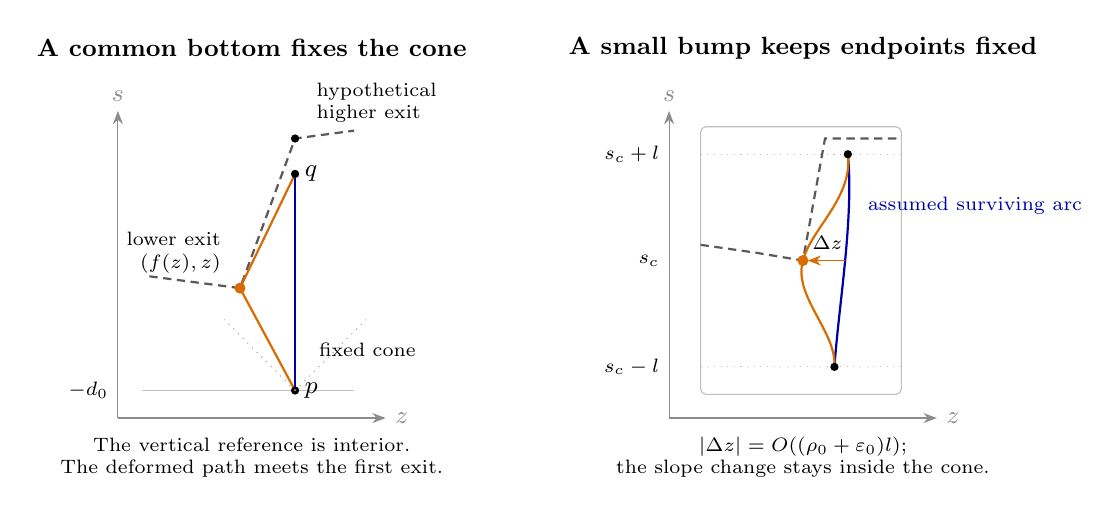
\begin{tikzpicture}[x=1cm,y=1cm,>=Stealth,
  every node/.style={font=\small},
  interior/.style={blue!65!black,thick},
  deformation/.style={orange!85!black,thick},
  boundary/.style={black!65,densely dashed,thick}]
 \begin{scope}
  \node[font=\small\bfseries] at (0,4.55) {A common bottom fixes the cone};
  \draw[->,black!45] (-1.7,-.15)--(-1.7,3.75) node[above] {$s$};
  \draw[->,black!45] (-1.7,-.15)--(1.7,-.15) node[right] {$z$};
  \draw[black!25] (-1.4,.2)--(1.3,.2);
  \node[left,font=\scriptsize] at (-1.7,.2) {$-d_0$};
  \draw[boundary] (-1.3,1.65)--(-.15,1.5)--(.55,3.4)--(1.3,3.5);
  \node[align=left,font=\scriptsize,anchor=west] at (.7,3.85)
       {hypothetical\\higher exit};
  \draw[interior] (.55,.2)--(.55,2.95);
  \draw[deformation] (.55,.2)--(-.15,1.5)--(.55,2.95);
  \fill (.55,.2) circle (1.5pt) node[right] {$p$};
  \fill (.55,2.95) circle (1.5pt) node[right] {$q$};
  \fill[orange!85!black] (-.15,1.5) circle (2pt);
  \node[anchor=east,align=right,font=\scriptsize] at (-.27,1.95)
       {lower exit\\$(f(z),z)$};
  \fill (.55,3.4) circle (1.5pt);
  \draw[black!35,dotted] (.55,.2)--(-.35,1.1);
  \draw[black!35,dotted] (.55,.2)--(1.45,1.1);
  \node[font=\scriptsize,anchor=west] at (.73,.72) {fixed cone};
  \node[font=\scriptsize,align=center] at (0,-.65)
       {The vertical reference is interior.\\The deformed path meets the first exit.};
 \end{scope}
 \begin{scope}[xshift=7cm]
  \node[font=\small\bfseries] at (0,4.55) {A small bump keeps endpoints fixed};
  \draw[->,black!45] (-1.7,-.15)--(-1.7,3.75) node[above] {$s$};
  \draw[->,black!45] (-1.7,-.15)--(1.7,-.15) node[right] {$z$};
  \draw[black!25,rounded corners=2pt] (-1.3,.15) rectangle (1.25,3.55);
  \draw[black!25,dotted] (-1.3,.5)--(1.25,.5);
  \draw[black!25,dotted] (-1.3,3.2)--(1.25,3.2);
  \node[left,font=\scriptsize] at (-1.7,.5) {$s_c-l$};
  \node[left,font=\scriptsize] at (-1.7,1.85) {$s_c$};
  \node[left,font=\scriptsize] at (-1.7,3.2) {$s_c+l$};
  \draw[boundary] (-1.3,2.05)--(-.6,1.95)--(0,1.85)--(.28,3.4)--(1.25,3.4);
  \draw[interior] (.4,.5) .. controls (.45,1.25) and (.65,2.4) .. (.57,3.2);
  \draw[deformation] (.4,.5) .. controls (.43,.95) and (-.13,1.4) .. (0,1.85)
       .. controls (.1,2.25) and (.64,2.65) .. (.57,3.2);
  \fill (.4,.5) circle (1.5pt);
  \fill (.57,3.2) circle (1.5pt);
  \fill[orange!85!black] (0,1.85) circle (2pt);
  \draw[->,orange!85!black,thin] (.53,1.85)--(.06,1.85);
  \node[font=\scriptsize,anchor=south] at (.31,1.87) {$\Delta z$};
  \node[font=\scriptsize,anchor=west,blue!65!black] at (.7,2.55) {assumed surviving arc};
  \node[font=\scriptsize,align=center] at (0,-.65)
       {$|\Delta z|=O((\rho_0+\varepsilon_0)l)$;\\the slope change stays inside the cone.};
 \end{scope}
\end{tikzpicture}

 \caption{Two uses of the fixed timelike cone, with one spatial
 coordinate shown.  Left: a common bottom and a point below the
 higher first exit would admit a path through the lower exit if
 the graph were too steep.  Right: a sufficiently narrow
 geodesic surviving across a small graph box can be deformed,
 with its endpoints fixed, through the central exit.  Both
 deformations contradict the intrinsic-diamond argument; the
 deformed paths use only the fixed timelike cone in the ambient chart.}
 \label{ex:figure}
\end{figure}

\subsection{The existential tests and their countable cover}

We have obtained uniform chart witnesses along a positive-measure
family of entire future geodesics. The remaining step is to localize
that family in one small branch tube, where a finite packet can affect
all observations. This localization must retain enough phase volume
for the two data sets compared later.

Return to the near-Kerr developments.  Use the single
$p_{10}$ neighborhood fixed in \Cref{prop:bg-package}, and
write $\mu_d$ for the section measure on $T\Sigma$ just
defined.  Fix a countable basis $\mathcal B$ of coordinate
balls in $T\Sigma$, with compact closures in members of a
countable atlas.  The centers and radii can be taken rational
in these coordinates, so the basis is fine enough for
Lebesgue differentiation with any smooth positive density.

\begin{definition}[Necessary existential extension tests]
\label{def:exit-test}
For $O\in\mathcal B$ and $B\in\N$, $B\ge1$, let
$E(O,B)\subset\Ueps$ consist of the data satisfying both
of the following requirements.
\begin{enumerate}[label=(\roman*)]
\item There is an extension of $M_d$ of the regularity and
      type specified in Definition~\ref{intro:extension}, and a measurable
      $S\subset O$ with
      \begin{equation}\label{ex:density-test}
                       \mu_d(S)>.99\,\mu_d(O),
      \end{equation}
      such that every seed in $S$ has finite full future
      lifetime.  There are at most $B$ precompact ambient
      charts $\psi_j:U_j\to V_j$ witnessing
      \Cref{ex:chart-witness} along each entire such geodesic,
      from $\Sigma$ to its full endpoint.  On the whole of
      every $V_j$, each of the metric norm, inverse metric
      norm, and Christoffel $L^2$ norm is at most $B$.
      At each point a selected chart has velocity norm at
      most $B$ and Euclidean distance to
      $\R^4\setminus V_j$ at least $1/B$.
\item There is an observation neighborhood $\mathcal N$ satisfying all three
      parts of \Cref{lem:bg-branch-tube} for this datum, with
      $\overline O\subset\mathcal N$ and the optical ordering chosen so that
      $v\to\infty$.
      One choice of its central branch track, compact state ranges,
      positive $p$ bounds, transverse earlier flow tube, interval $J$,
      observation boxes, admissible launch patch, unbounded sequence of
      $T$, and constants $u_2,c_2,c_0$ serves every seed in $\overline{\mathcal N}$.
      In particular,
      the entry-to-observation portions fit
      \eqref{bg:experiment-domain} with its outer margins and positive
      slice-length bound. The admissible patch has the low-order ray
      and collar properties specified before \Cref{lem:bg-branch-tube}.
\end{enumerate}
All tube constants, charts, patches, and subsequences in this
definition are existential witnesses for the given datum.
They are not additional countable indices and are not
required to work in a neighborhood of that datum.
\end{definition}

The measurable good family in this definition may depend on
the extension.  For later averaging, whenever its point and
velocity satisfy several chart conditions, select the least
chart index.  The finite collection of coordinate margin and
velocity conditions is Borel on the interior unit shell, so
this gives a measurable selector, also when it depends on the
momentum.  No closedness assertion about $E(O,B)$ is made.

\begin{proposition}[Countable cover of all future extensions]
\label{prop:exit-cover}
Every datum in $\Ueps$ admitting a future
$C^0\cap W^{1,2}_{\mathrm{loc}}$ extension belongs to some
$E(O,B)$.  Consequently the extendible set is precisely
\[
                  \bigcup_{O\in\mathcal B}\ 
                         \bigcup_{B=1}^{\infty}E(O,B).
\]
This cover includes extensions whose actual exit occurs
after first runout from the comparison development.
\end{proposition}

\begin{proof}
Fix such a datum and extension.  \Cref{prop:exit-family}
provides a measurable family $S_*$ of positive $\mu_d$ measure,
finite full lifetimes, and one finite set of ambient chart
witnesses.  By \Cref{prop:bg-runout}, every seed in $S_*$
crosses the comparison cylinder and its first comparison
runout is a branch or a corner.  The corner subset is null.
The inputs here are precisely the finite-full-lifetime
classification of \cite[\CompanionRef{foundation}{cmp:classification}]{KerrCTwo} and the
section-volume corner removal of
\cite[\CompanionRef{signed}{test:corner-null}]{KerrCOne}; the latter uses only the
low-order corner estimates of
\cite[\CompanionRef{foundation}{cmp:corner-ratios}]{KerrCTwo}.  These statements have neither a
regular-extension hypothesis nor a curvature bound along
the selected seed.

Choose a density point $w$ of $S_*$ outside that null subset,
with $w\in S_*$.  It is a branch seed.  Apply
\Cref{lem:bg-branch-tube} and, if necessary, interchange the
optical labels.  This gives an open seed neighborhood $\mathcal N$ of
$w$ with all the tube, footprint, and finite-domain
properties in \Cref{def:exit-test}(ii). These are consequences of
the background estimates and hold independently of the extension
chart witnesses.

By density and the fine countable basis, choose $O\ni w$
with $\overline O\subset\mathcal N$ and
$\mu_d(S_*\cap O)>.99\mu_d(O)$.  To justify using countably
many balls, small balls centered at a density point can be
enlarged by an arbitrarily small relative amount to balls
with rational center and radius.  Smooth positivity of the
density keeps their measures comparable, so their relative
complement measure still tends to zero.  Set $S=S_*\cap O$.
Choose an integer $B$ at least the number of the ambient
charts, all their bounds, and the reciprocal of their common
margin.  This proves $d\in E(O,B)$.

Every observation invoked here lies strictly before first
runout from the comparison region.  The finite full lifetime
and ambient chart witnesses were obtained independently for
the entire geodesic in $M_d$.  Thus first runout is used only
to locate earlier observations; it need not be the ambient
exit.  Finally the reverse inclusion in the displayed union
is part of \Cref{def:exit-test}(i).
\end{proof}

\section{Preparing exact data and a double-null template}
\label{pk:section}

Fix a smooth datum $d\in\Ueps$, a branch tube together with all its
witnesses from \Cref{lem:bg-branch-tube}, and a finite integer $m\ge10$.
After interchanging the optical labels if necessary, its central
track has $u\to u_*\in\R$ and $v\to\infty$. All constants in this
section may depend on this fixed datum and tube. Write $\mathcal N$ for its seed
neighborhood. Use the witnessing constants $u_2>u_*$, $c_2>0$, and
$c_0>0$, interval $J$, observation boxes $\mathcal Q_T$, launch patch,
and unbounded sequence of $T$ throughout. The finite experiment uses
\begin{equation}\label{pk:domain}
 \mathcal D_T=\left\{0\le t\le L_T:=\frac{T+u_*}{2}+c_0,
 \quad u+\frac{c_0t}{T}\le u_2,
 \quad v+\frac{c_0t}{T}\le T+c_2\right\}.
\end{equation}
We construct on small enlargements and restrict inside their margins.
The tube, the observation interval $v\in T+J$, and its angular
footprint fit these margins along an unbounded sequence of $T$.
The slice $x$-intervals have a positive lower length bound. Put
\begin{equation}\label{pk:scales}
 \alpha=\kappa/4,\qquad \amp=e^{-\alpha T},
 \qquad \lambda=e^{\zeta T}.
\end{equation}
The small constant $\zeta>0$ is chosen only after all finite base
orders and rate tolerances. In particular, $\amp$ is substantially
larger than the square root of the lapse in the observation region.

Use the observation boxes $\mathcal Q_T$ and their fixed enlargements
from \Cref{lem:bg-branch-tube}. They contain all hitting positions of
the seed-neighborhood closure $\overline{\mathcal N}$ at $v\in T+J$. Their feet lie in
one compact subpatch of the admissible launch patch, with a common
interior margin along the selected sequence. Choose the launch bump
below to be at least one on a neighborhood of this entire foot set.

\begin{proposition}[Packet preparation]\label{prop:packet-preparation}
For every finite $m\ge10$, finite jet budget $N$, positive loss
tolerance $\eta_{\rm out}$, and $0<\nu<1$, one can choose $\zeta>0$ and
finite construction orders so that the following objects exist
for arbitrarily large $T$ along the indicated sequence.
\begin{enumerate}
\item There are exact smooth complete vacuum data $d_T\in\Ddata$
on the whole bridge with $p_m(d_T-d)\to0$. They agree with $d$ on
the other end, the connecting region, and an expanding protected
ball on the selected end. The permitted exterior correction tail
is retained.
\item An exact exterior evolution of $d_T$ reaches the required
part of $\mathcal S$, with overlapping collars and strict outflow
margins. In the fixed background wave-map description its entry
spacetime jets differ from $g+h^p$ by $O(\amp^2e^{\eta_{\rm out} T})$.
Here
\begin{equation}\label{pk:packet}
 h^p=\amp\,\operatorname{tr.rev.}_g\operatorname{Re}
       \left(e^{i\lambda v}\sum_{j=0}^{J_*}\lambda^{-j}p_j\right).
\end{equation}
The leading coefficient is real, trace-free, and annihilates
$L_0$. On the entire observation box $\mathcal Q_T$,
\begin{equation}\label{pk:screen-lower}
 |(p_0)_{AB}|_\gamma\ge e^{-o(T)}.
\end{equation}
At every fixed required base order the ordinary mixed coordinate jets
of the normalized amplitude components are $e^{o(T)}$, and the linearized Ricci and gauge errors have
arbitrarily high inverse-frequency accuracy.
\item There is a metric $\bar g$ exactly of double-null form, with
fields $\bar\gamma,\log\bar{\mathcal A},\bar b$ and their exact
geometric derived fields. Through order $N$, its differences from
the background fields, including $q^{-1}\partial_vb$, are
$O(\amp e^{\eta_{\rm out} T})$. Its defects in the null structure and
angular equations \eqref{dn:D2}--\eqref{dn:D3} are
$O(\amp^2e^{\eta_{\rm out} T})$. If the actual exterior induced data are
written in double-null coordinates initialized by the background
values on $\mathcal S$, their full entry jets differ from this
template by the same quadratic bound.
\end{enumerate}
All entry discrepancies and all template changes and defects vanish
for $v<(1-\nu)T$. Any additional finite initial or residual jet
buffers may be included in $N$. Positive frequency powers at these
base orders are independent of the later orders used to improve
linear accuracy. At the finitely many high entry orders ultimately
requested by \Cref{thm:dn-comparison}, the actual fields have
$e^{o(T)}$ bounds.
\end{proposition}

For the proof, choose an internal loss
$0<\eta<\min\{\eta_{\rm out},\alpha/4\}$. The bootstrap estimates
below are obtained with this smaller loss, after splitting it among
the finitely many steps, and then imply the stated bounds with
$\eta_{\rm out}$. This distinction permits any prescribed positive
output tolerance.

\subsection{The homogeneous linear hierarchy and its footprint}

Complex Gaussian beams and their superpositions were developed by
Ralston, Tanushev, and Liu--Runborg--Tanushev
\cite{Ralston1982,Tanushev2008,LiuRunborgTanushev2013}.
The companion construction used here also enforces the Einstein
wave-gauge constraints and supplies the fixed-order bounds on
intervals growing with $T$. We retain the hierarchy and matching
estimates needed for the larger amplitude.

We use the amplitude-independent constrained construction of
\cite[\CompanionRef{signed}{bg:packet}, \CompanionRef{signed}{bg:amplitude-independent}]{KerrCOne}, whose hypotheses are
the background coefficient estimates and a branch tube; it expressly
requires no bound on curvature in an observer's parallel frame.
Its proof uses the hierarchy and beam interfaces of
\cite[\CompanionRef{foundation}{pk2:hierarchy}, \CompanionRef{foundation}{pk2:escape}, \CompanionRef{foundation}{pk2:beam-proposition}]{KerrCTwo}.
We specify the part needed for a signal on a whole footprint.

Let $P$ be the background linearized reduced vacuum operator on
trace-reversed two-tensors, $C_g=\divg_g$, and $P_1$ the induced
one-form wave operator. The Ricci-flat Bianchi identity is
$C_gP=P_1C_g$. For
\[
 k_v=g^{-1}\dd v=-a^{-1}L_0,\qquad
 K_vp=p(k_v,\cdot),\qquad
 \mathcal T=2\nabla_{k_v}+\square_gv,
\]
the coefficients solve
\begin{equation}\label{pk:hierarchy}
 i\mathcal T p_j+Pp_{j-1}=0,\qquad
 iK_vp_j+C_gp_{j-1}=0,\qquad p_{-1}=0.
\end{equation}
Work on $-v\le u\le u_f$, where $u_f>u_2$. Multiplication of the
homogeneous transport by $-a/2$ gives
$\nabla_{L_0}+\tfrac12\tr_\gamma\chi_0$. In the normalized slots
$(a^{-1/2}L_0,a^{-1/2}L_1,\partial_\theta)$ its constant diagonal
weights are $\kappa(n_0-n_1)/2$: here $n_i$ counts the arguments of
type $a^{-1/2}L_i$ in a covariant two-tensor component, so
$n_0+n_1\le2$. The normalized connection formulas
in \cite[\CompanionRef{foundation}{pk2:coefficients}]{KerrCTwo} make the hierarchy triangular from
higher weights to lower weights. Nonnegative weights are prescribed
at $u=-v$, with the components containing an $L_0$ argument fixed
by the gauge equation;
negative weights $1A,11$ are prescribed at $u_f$ and transported
backwards. The sign of each weight is favorable in its prescribed
direction. Higher differentiated coefficients multiply already
controlled lower jets, so each finite transport induction costs
only $e^{o(T)}$. The angular characteristic and inverse
characteristic jets have this same bound, including derivatives
of the moving initial edge $u=-v$.

For the free leading angular data, orthonormalize a fixed smooth local
coframe using the entry screen metric, obtaining $e^1,e^2$. Uniform
low nondegeneracy and the fixed higher coefficient bounds give
$e^{o(T)}$ jets for this coframe at every fixed order. Use the real
trace-free unit polarization
$2^{-1/2}(e^1\otimes e^1-e^2\otimes e^2)$, multiplied by the bump
that is at least one on a neighborhood of the complete foot set.
Take zero free angular data at higher levels.
The initial polarization exists on the one small chart patch; no
global choice of a nonvanishing trace-free tensor on $\Sph$ is
required. The leading transport is real. It preserves trace and
annihilation of $k_v$, and acts on the positive screen quotient by
isometric parallel transport times a real nonzero scalar. The
scalar and its reciprocal are $e^{o(T)}$, since its logarithm is
an integral of the expansion coefficient. Thus the positive bump
gives \eqref{pk:screen-lower} at every point whose foot lies in
the chosen foot set, uniformly throughout $\mathcal Q_T$.
There is no phase adjustment at a single observation point.

Gauge compatibility follows directly by conjugating
$C_gP=P_1C_g$ with $e^{i\lambda v}$: once preceding gauge defects
vanish, the next defect satisfies homogeneous one-form transport
with zero initial value. Terminal prescriptions for negative
weights create no additional condition, since $K_v$ contracts
precisely an $L_0$ argument. Smooth zero extension away from the launch
band is therefore allowed. For any fixed base order, truncating
\eqref{pk:hierarchy} far enough gives scaled reduced-wave and gauge
residuals $\amp\lambda^{-M}e^{o(T)}$ for any prescribed $M$.

The exterior transfer of \cite[\CompanionRef{signed}{bg:packet}, \CompanionRef{signed}{bg:amplitude-independent}]{KerrCOne} supplies a real
lab-coordinate tensor $h^B$, including the factor $\amp$, with
\begin{equation}\label{pk:beam-base}
 \|h^B\|_{C^s}\le\amp\lambda^{s+3/2}e^{o(T)}.
\end{equation}
Its wave, gauge, and entry-matching residuals can simultaneously be
$\amp\lambda^{-M}e^{o(T)}$. The geometric hypotheses of that lemma
hold here: the prepared optical covectors have escaping backward
rays; the entry, horizon, and initial-slice crossings are
transverse; the fixed-depth collar has uniform low nondegeneracy;
and all fixed higher coefficient and flow jets are subexponential.
These are coefficient properties of the fixed background from
\Cref{prop:bg-package}. The fixed small launch patch is chosen
using only these low bounds. It need not shrink as approximation
orders increase. For each prescribed relative annulus tolerance,
a larger fixed far threshold and then large $T$ place the initial
support in that thin annulus, uniformly for all centers in the
patch; this is the backward-ray estimate in
\cite[\CompanionRef{foundation}{pk2:escape}]{KerrCTwo}.

We recall why the positive exponent in \eqref{pk:beam-base} is
independent of later accuracy. The constrained beams are integrated
over a fixed three-dimensional center patch with normalization
$(\lambda/2\pi)^{3/2}$. Each of $s$ differentiations costs at most
$\lambda$, while every finite phase and amplitude coefficient is
$e^{o(T)}$ after its displayed inverse powers have been extracted.
Taking absolute center integrals gives \eqref{pk:beam-base}.
For each beam center $c$, let $P_c,Q_c\in\mathbb C^{3\times3}$ be
the position and momentum differential blocks of the Hamiltonian ray
map acting on the initial complex phase graph. If $M_0$ is its
symmetric initial phase Hessian with positive imaginary part, then
$P_c(0)=\Id$ and $Q_c(0)=M_0$. The imaginary Hessian remains positive
through real caustics by the symplectic identity
$P_c^*Q_c-Q_c^*P_c=2i\operatorname{Im}M_0$; it gives a
subexponential inverse of the complex position projection.
At a fixed transverse Taylor degree $d$, homogeneous amplitude-jet
transport in ray-comoving coordinates is the central amplitude
transport. Returning to fixed coordinates also applies the $d$-fold
symmetric tensor power of $J_c(t,s)^{-{\mathsf t}}$, where
$J_c(t,s)=P_c(t)P_c(s)^{-1}$. The bounds for $P_c$ and $P_c^{-1}$
keep this factor subexponential for every fixed $d$. Thus same-degree
jet couplings remain controlled when the finite accuracy order is raised.
An uncancelled Taylor degree gains
$\lambda^{-1/2}e^{o(T)}$ by Gaussian integration. Increasing the
finite Taylor and transport orders therefore improves only
inverse accuracy. The entry Gaussian expansion is triangular in
amplitude level, and its new free contraction-kernel value matches
the corresponding $p_j$. These are precisely the fixed-base
assertions proved in \cite[\CompanionRef{foundation}{pk2:beam-proposition}]{KerrCTwo}. Linearity makes
them valid at the amplitude \eqref{pk:scales}.

\subsection{Exact constraints and exterior propagation at the new amplitude}

Localized deformation of the vacuum constraints was developed by
Corvino--Schoen and Chru\'sciel--Delay
\cite{CorvinoSchoen2006,ChruscielDelay2003}. Here the correction fixes
an inner ball and retains a noncompact decaying tail. Its support and
weighted bounds must remain explicit, since they determine both
closeness of the complete data and the first time the perturbation can
reach the interior.

In the selected exterior, $t_e$ denotes exterior time, $z$ lab
position, and $C(t_e)$ the drift center; its co-moving radius is
$r_{\rm co}=|z-C(t_e)|$.
Write $t_T\asymp T$ for the exterior time corresponding to the
launch cylinder and $z_*=C(t_T)$ for its lab drift center. Choose
a small relative gap $\beta>0$ with
$s_*:=\sup|C'|<1-2\beta$, and set
\begin{equation}\label{pk:protected}
 \rho_T=(1-2\beta)t_T,\qquad |z-z_*|<\rho_T.
\end{equation}
The thin launch annulus lies outside this protected ball with a
margin. In the variables $y=(z-z_*)/\rho_T$, keep Cartesian metric
components unchanged and multiply second-fundamental-form
components by $\rho_T$. Both constraints are then multiplied by
$\rho_T^2$. Extending the unperturbed rescaled datum smoothly
inside the unit ball, without imposing a constraint there, gives
a perturbation of flat data of size $O_s(T^{-1})$ at every fixed
symbol order.

Here is the exact constraint-solver interface being used. For
$s\ge3$, let
\[
 \|f\|_{H^j_\ell}=\|f\|_{H^j(B_2)}+
  \sup_{R\ge1}R^\ell
       \|f(R\,\cdot)\|_{H^j(\{1<|y|<2\})},\qquad
 X^s=H^{s+2}_1\oplus H^{s+1}_2,\quad Y^s=H^s_4.
\]
Here $H^j_\ell$ is the class of locally $H^j$ fields with finite
displayed norm. In particular, the weight-one and weight-two factors
include fields with saturated $|y|^{-1}$ and $|y|^{-2}$ decay at
infinity; these classes are larger than the closures of compactly
supported fields.
\cite[\CompanionRef{foundation}{pk:constraint-nonlinear}, \CompanionRef{foundation}{pk:constraint-linear}]{KerrCTwo} give a bounded
operator $\mathcal K:Y^s\to X^s$ preserving exterior support, with
$P_{\rm flat}\mathcal Kz=z$ for exterior-supported $z$, where
$P_{\rm flat}$ is the flat constraint linearization. They also give a contraction for the nonlinear
constraints when one finite background-plus-defect base norm is
small. For the smooth compact beam deformation and the smooth
background with all-order symbol bounds used here, the output is
smooth, zero inside the protected ball, and has all-order symbol
tails of weights one and two. The iteration sources may themselves
have noncompact exterior-supported tails. There is no
moment condition on the original defect and no fixed-charge
requirement. Smoothness at higher orders requires bounded higher
symbol norms, not their smallness.

Take $s$ large enough for $m$ and all requested comparison buffers.
Let $d_B$ be the rescaled beam seed, and let $f_B$ be its exterior
constraint defect extended by zero inside the ball. Thus $f_B=\Phi(d_B)$
outside the ball; the artificial interior need not satisfy the constraints.
Linearize the constraint map at the actual rescaled vacuum background
on the exterior. Gauss--Codazzi expresses this first variation as a
linear combination of the reduced-wave residual and one derivative
of the linear gauge defect, with smooth background coefficients.
Include gauge-defect jets through $s+1$ among the fixed base orders
before choosing $\zeta$. Taylor expansion around that background then gives
\begin{equation}\label{pk:exterior-defect}
 \|f_B\|_{Y^s}
 \le \operatorname{poly}(T)e^{o(T)}
      \bigl(\amp\lambda^{-M}+\amp^2\lambda^{P_*}\bigr).
\end{equation}
Here and below $P_*$ depends on the fixed base orders alone.
The flat operator is reserved for the correction iteration below;
the linear cancellation in \eqref{pk:exterior-defect} uses the actual
background.
The rescaled seed base norm is
$O_s(T^{-1})+\operatorname{poly}(T)\amp\lambda^{P_*}e^{o(T)}$.
Choosing $\zeta P_*<\alpha/2$ makes it small. The inverse-metric
and contraction balls of the cited proposition consequently
apply for large $T$. Equivalently, solve
\[
 z=-f_B-N_{d_B}(\mathcal Kz),\qquad
 N_{d_B}(w)=\Phi(d_B+w)-\Phi(d_B)-P_{\rm flat}w.
\]
The Lipschitz constant is at most $1/2$, and the correction has
the size of \eqref{pk:exterior-defect}. The defect is smoothly zero
near the inner boundary, and the support-preserving inverse and
nonlinear iteration keep the correction zero on the entire inner
side. Since $P_{\rm flat}\mathcal Kz=z$, the corrected constraint
is $\Phi(d_B+\mathcal Kz)=\Phi(d_B)-f_B$, hence zero outside the ball.
On the inner side $N_{d_B}(\mathcal Kz)=0$ because the correction and
all its jets vanish. Undoing the rescaling and restoring the original
vacuum datum inside therefore gives smooth exact data on the complete
bridge.

The metric stays positive and uniformly comparable to the original
complete metric. Weighted differentiation after translation and
rescaling costs only powers of $T$. For example, the seed contributes
at most $\operatorname{poly}(T)\amp\lambda^{m+5/2}e^{o(T)}$ to
$p_m$, and the correction contributes the same polynomial type of
loss times \eqref{pk:exterior-defect}. Thus $p_m(d_T-d)\to0$.
Every higher weighted seminorm of each individual $d_T$ is finite
by the all-order symbol assertion. The exterior tail and any charge
change remain part of $d_T$.

Initialize the exact exterior wave-map evolution with target $g$.
Choose initial lapse and shift as for $g+h^B$; the corrected second
fundamental form and exact gauge determine the remaining normal
metric jets by a uniformly noncharacteristic algebraic system.
Its linearization matches the constrained beam, so its discrepancy
has size \eqref{pk:exterior-defect}. Further normal jets follow
from the reduced equations. Agreement on the protected region is
exact.

We now justify the new amplitude in the exterior propagation.
For a lab-component metric change $H$, the reduced equation has
the form
\begin{equation}\label{pk:exterior-operator}
 \mathcal R_e(H)_n=(\mathcal L_eH)_n+
 \bigl((g+H)^{-1}-g^{-1}\bigr)^{\rho\sigma}
       \partial_\rho\partial_\sigma H_n+
 \mathcal Q_n(H,\partial H),
\end{equation}
where $\mathcal Q$ starts quadratically and has total derivative
order at most two, with fixed differentiated coefficients
$e^{o(T)}$. On the uniformly nondegenerate exterior domain,
$\mathcal R_e(h^B)$ has the size in
\eqref{pk:exterior-defect}; there is no small interior lapse in
this assertion. Write $H=h^B+F$ and bootstrap sufficiently high
mixed lab-coordinate error energies by $e^{-\alpha T}$.
Retain the actual metric $g+h^B+F$ in the highest-order wave
operator. Every other nonlinear error term has an additional
packet or error factor. Put its highest error derivative in
$L^2$ and its lower factors in $L^\infty$ using a fixed Sobolev
buffer. These factors are exponentially small, so the nonlinear
energy rate is exponentially small.

The individual exterior estimate proved in
\cite[\CompanionRef{signed}{prep:exterior-rate-section}, \CompanionRef{signed}{prep:amplitude-independent-exterior}]{KerrCOne}
uses finite shrinking computing slices
\begin{equation}\label{pk:outer-cutoff}
 r_{\rm co}<R_{\rm out}(t_e)
 =C_{\rm out}(1+T)+V_{\rm out}(t_T+C_2-t_e),\qquad
 V_{\rm out}>\sup_{\rm causal}|\dd r_{\rm co}/\dd t_e|.
\end{equation}
Their radii are $O(T)$ on the finite comparison interval, and the side
is strictly outgoing. The physical correction tail outside this
computing region remains part of the complete initial datum. On these
slices the estimate for square-root energies at exact orders $j$ reads
\begin{equation}\label{pk:exterior-energy}
 E_j'\le r_e E_j+C_je^{o(T)}\sum_{k<j}E_k+\mathcal F_j,
 \qquad \mathcal F_j\le
 \operatorname{poly}(T)e^{o(T)}
 (\amp\lambda^{-M}+\amp^2\lambda^{P_*}).
\end{equation}
For precision, its arbitrarily small integrated rate is available
at this amplitude for the following reason. The actual scalar
stress energy, with future slice normal and a small positive mass,
has nonnegative outflow flux. Its same-order linear rate uses only
first and second lab metric derivatives, which are small at large
co-radius and uniformly bounded elsewhere. Higher background
derivatives multiply lower exact-order energies. The first-arrival
estimate, valid also for the noncompact correction since it is zero
in the protected ball, is
\begin{equation}\label{pk:first-arrival}
 (1-2\beta)t_T\le (1+\delta_R)t_e+O(R)
                              +s_*|t_T-t_e|,
 \qquad \delta_R\longrightarrow0.
\end{equation}
Indeed before its first hit of a fixed large co-radius $R$, a
causal path from the changed support has lab speed at most
$1+\delta_R$; its endpoint is within $O(R)$ of $C(t_e)$.
The fixed gap $1-s_*>0$ in \eqref{pk:first-arrival} implies that
the change cannot see the bounded-rate region before
$t_e\ge t_T-\beta'T$, where $\beta'>0$ can be made arbitrarily
small by decreasing $\beta$ and increasing $R$. The localized
beam obeys the same conclusion. Thus
\[
 \int_0^{t_T+C_2}r_e\,\dd t_e\le\eta' T
\]
for any prescribed $\eta'>0$. The bounded compact rate is
independent of the chosen far threshold. Increasing that threshold
later for the thin annulus therefore causes no conflict. The
choices also protect the entire earlier entry interval
$v<(1-\nu)T$.

Remove the common rate from \eqref{pk:exterior-energy}.
Iteration of the finite lower-triangular hierarchy introduces only
a polynomial of fixed degree in $Te^{o(T)}$, hence another
$e^{o(T)}$ factor. Allocating the finitely many rate losses in
advance, then choosing $\zeta$ small and $M$ large, gives
\begin{equation}\label{pk:wave-entry}
 \|g_T^{\rm ext}-g-h^p\|_{C^N(\mathcal S)}
                         \le\amp^2e^{\eta T}.
\end{equation}
The bound first holds with $h^B$ on the exterior; the fixed-depth
coordinate transition, spacetime trace with finite buffers, and
linear entry matching replace it by $h^p$. It strictly improves
the bootstrap since $2\alpha-\eta>\alpha$ after choosing losses
small. Local reduced-wave restart inside enlarged outflow margins
gives the entire finite exterior. Constraint and gauge propagation
give exact vacuum. These continuation statements are the ones
used in \cite[\CompanionRef{foundation}{in:continuation}, \CompanionRef{foundation}{cmp:development}, \CompanionRef{foundation}{pk2:exterior-proposition}]{KerrCTwo}.
This argument is the individual exterior comparison; it uses no
deep wave-coordinate nonlinear estimate.

\subsection{Linear optical coordinates and the relative shift}

The exact evolution from the entry cylinder will use two optical
functions and angles having the \emph{same values} as the background
ones on $\mathcal S$. Choose the neighboring eikonal roots and
transport the angles so that the shift in direction $1$ is zero.
The entry surface consequently retains the labels $u+v=0$.
Only the linearized coordinate change is needed to construct the
comparison template.

\begin{lemma}[Linear optical gauge]\label{lem:packet-linear-gauge}
Let $Z=(z^0,z^1,z^\theta)$ be the variations of the coordinate
functions, with $Z=0$ on $\mathcal S$, for the input $h^p$.
In unnormalized components $h^p_{ij}=h^p(L_i,L_j)$ and
$h^p_{iA}=h^p(L_i,\partial_A)$, they obey
\begin{equation}\label{pk:linear-optical}
 \begin{aligned}
 \partial_vz^0&=-\frac{h^p_{11}}{2a},&
 L_0z^1&=-\frac{h^p_{00}}{2a},\\
 \partial_vz^\theta
 &=b\partial_vz^0+a\gamma^{-1}\dd_\theta z^0
                         +\gamma^{-1}h^p_{1\cdot}.
 \end{aligned}
\end{equation}
For every fixed number of angular derivatives and $r$ total
longitudinal derivatives,
\begin{equation}\label{pk:coordinate-gain}
 |\partial_{u,v}^{r}\partial_\theta^sZ|
                      \le\amp\lambda^{r-1}e^{o(T)}.
\end{equation}
The fixed-new-label metric variation is $k=h^p-\Lie_Zg$.
Its field variations $k_\gamma,k_H,k_b$, where $H=\log\mathcal A$,
and the relative derivative $q^{-1}\partial_vk_b$ satisfy
\begin{equation}\label{pk:relative-linear}
 \|(k_\gamma,k_H,k_b,q^{-1}\partial_vk_b)\|_{C^s}
                        \le\amp\lambda^{P_s}e^{o(T)}
\end{equation}
at every fixed required order. The exponents $P_s$ depend only on
that order, not on subsequent inverse-accuracy choices.
\end{lemma}

\begin{proof}
The inverse metric is
\[
 g^{-1}=-a^{-1}(L_0\otimes L_1+L_1\otimes L_0)
                        +\gamma^{AB}\partial_A\otimes\partial_B.
\]
Linearization of $g^{-1}(\dd u,\dd u)=0$ gives
$-a^{-2}h^p_{11}-2a^{-1}\partial_vz^0=0$; the equation for $v$
is analogous. For the angle condition
$g^{-1}(\dd u,\dd\theta^A)=0$, the metric variation contributes
$a^{-1}\gamma^{AB}h^p_{1B}-a^{-2}b^Ah^p_{11}$.
The coordinate variations contribute
$\gamma^{AB}\partial_Bz^0-a^{-1}b^A\partial_vz^0
-a^{-1}\partial_vz^A$.
Substitution of the first eikonal equation gives the last equation
in \eqref{pk:linear-optical}, including its sign and factor.

To see the gain in \eqref{pk:coordinate-gain}, a typical term in
the first equation has the form
$\amp e^{i\lambda v}f(u,v,\theta)$ with fixed coefficient jets
$e^{o(T)}$. At fixed $u,\theta$,
\begin{equation}\label{pk:oscillatory-integral}
 \begin{split}
 \int_{-u}^{v}e^{i\lambda s}f(u,s,\theta)\,\dd s
 ={}&\frac{e^{i\lambda v}f(u,v,\theta)
          -e^{-i\lambda u}f(u,-u,\theta)}{i\lambda}\\
 &-\frac1{i\lambda}
           \int_{-u}^{v}e^{i\lambda s}\partial_sf(u,s,\theta)\,\dd s.
 \end{split}
\end{equation}
The interval has length $O(T)$; its polynomial length is absorbed
in $e^{o(T)}$. Differentiation in $u$ differentiates the lower
endpoint and its coefficient as well as the integral. Each
longitudinal derivative costs at most one additional $\lambda$,
including the phase $e^{-i\lambda u}$ at that endpoint. Angular
derivatives do not differentiate the phase. This proves the
assertion for $z^0$ with arbitrary fixed differentiated orders.
The relative coefficient $h^p_{11}/a$ is a normalized tensor
entry, so no inverse lapse was lost.

For $z^1$, the leading $00$ coefficient is identically zero:
$p_0$ annihilates $L_0$, and trace reversal leaves the same-null
$00$ component unchanged because $g_{00}=0$. Thus $h^p_{00}/a$ already has a factor
$\lambda^{-1}$. Integration along $L_0$ keeps $v$ fixed, with
angular characteristic jets and inverse jets $e^{o(T)}$.
Differentiating its moving initial point $u=-v$ has the same
endpoint rule as above. Its interval length is again $O(T)$.
This proves the bound for $z^1$ without requiring oscillation in
the direction of that integration.

For the angular equation, $h^p_{1A}$ is $\sqrt a$ times a
normalized oscillatory coefficient, so \eqref{pk:oscillatory-integral}
applies. The term $a\gamma^{-1}\dd_\theta z^0$ already has the
inverse-frequency gain. Integrating its length costs only
$e^{o(T)}$, also at differentiated orders. Finally,
\[
 \int_{-u}^{v}b\partial_vz^0\,\dd v
   =bz^0\big|_{-u}^{v}-\int_{-u}^{v}(\partial_vb)z^0\,\dd v,
\]
where the lower value of $z^0$ is zero. All derivatives of
$\partial_vb$ retain their factor $a$, and the remaining
coefficients have subexponential fixed jets. This proves
\eqref{pk:coordinate-gain} for the angles as well.

For explicit field formulas set $W=z^\theta-z^0b$, an angular
vector field. A direct Lie derivative gives
\begin{equation}\label{pk:linear-fields}
 \begin{aligned}
 k_\gamma&=h^p_{AB}-2z^0\chi_0-2z^1\chi_1-\Lie_W\gamma,\\
 k_H&=-a^{-1}h^p_{01}-Z\log a-L_0z^0-\partial_vz^1,\\
 k_b&=-\gamma^{-1}h^p_{0\cdot}
       +\partial_uW+[b,W]-z^1\partial_vb
                                      -a\gamma^{-1}\dd_\theta z^1.
 \end{aligned}
\end{equation}
Indeed $(\Lie_Zg)_{AB}=2z^0\chi_0+2z^1\chi_1+\Lie_W\gamma$,
whereas
$(\Lie_Zg)(L_0,L_1)=-Za-a(L_0z^0+\partial_vz^1)$.
The $0A$ component is
$\gamma_{AB}(\partial_uW+[b,W]-z^1\partial_vb)^B
-a\partial_Az^1$. The linear double-null component conditions
$k_{11}=k_{00}=k_{1A}=0$ follow from
\eqref{pk:linear-optical}. Hence
$k_H=-k(L_0,L_1)/a$ and $k_b=-\gamma^{-1}k_{0\cdot}$, which
give \eqref{pk:linear-fields}. All displayed divisions by $a$
are relative factors: $h^p_{01}/a$ is normalized and
$\partial a/a=\partial\log a$ has the given coefficient bounds.
Thus these three field variations have the claimed fixed
positive frequency powers. This argument alone does not estimate
$q^{-1}\partial_vk_b$; that relative derivative is obtained next.

Let $X_i$ denote the exact linear variation of $\xi_i$ under $k$.
The torsion sum identity gives $X_0+X_1=\dd_\theta k_H$.
The linearized vacuum identities are available with arbitrary
linear accuracy: diffeomorphism covariance on the vacuum
background gives
\[
 D\Ric_g(\Lie_Zg)=\Lie_Z\Ric(g)=0.
\]
The algebraic and differential steps turning Ricci components into
the null equations can lose fixed powers of $q^{-1}$, but only
on the \emph{linear residual}. On \eqref{pk:domain} these powers
are $e^{C_sT}$ for a fixed $C_s$. After $\zeta$ is fixed, increasing
$M$ in $\amp\lambda^{-M}$ makes this residual smaller than any
prescribed exponential at all finitely many required orders.

Use specifically the shift-free direction-$1$ torsion equation
of \cite[\CompanionRef{foundation}{in:vacuum}]{KerrCTwo}. Its linearization is
\begin{equation}\label{pk:linear-torsion}
 (\partial_v+\tau_1)X_0
   =\delta\beta_1+\delta\tau_1\,\xi_1
                     +\tau_1\dd_\theta k_H+\mathfrak r_{
                     \rm lin}.
\end{equation}
Here
\[
 \delta\chi_1=\tfrac12\partial_vk_\gamma,\qquad
 \delta\tau_1=\tr_\gamma\delta\chi_1
                 -\gamma^{AC}k_{\gamma,CD}\gamma^{DB}\chi_{1,AB},
\]
and
\[
 \delta\beta_1=\divg_\gamma\delta\chi_1
 -\dd_\theta\delta\tau_1+(\delta\divg_\gamma)\chi_1.
\]
The operator variation in the last term uses only $k_\gamma$
and one angular derivative of $k_\gamma$. Thus the entire source
in \eqref{pk:linear-torsion} has already been estimated using
\eqref{pk:linear-fields}; it uses neither $X_i$ nor an unknown
relative shift derivative. Also
\[
 \int_{-u}^{v}|\tau_1(u,s,\theta)|\,\dd s
       \le C\int_{-u}^{v}(q+g_1(s))\,\dd s\le C.
\]
At the moving entry edge $q=q_0$, the initial $X_0$ is a finite-jet
expression with no small denominator. It has size
$\amp\lambda^{P_s}e^{o(T)}$. The integrating-factor estimate
therefore gives this bound for $X_0$, and then for $X_1$.
Commutation with $u$ and angular derivatives leaves the same top
transport coefficient; differentiated coefficients multiply lower
already estimated $X_0$ jets. Entry terms from differentiating
$v=-u$ are controlled by the differentiated entry data, with normal
jets also given by the equation. Derivatives in $v$ are recovered
from \eqref{pk:linear-torsion}. This proves the finite-order
assertion without a shifted transport containing an unknown $k_b$.

Finally linearize the defining shift relation. It gives exactly
\begin{equation}\label{pk:relative-shift}
 \begin{split}
 q^{-1}\partial_vk_b={}&\mathcal A\gamma^{-1}(X_1-X_0)\\
 &+\bigl(k_H\Id-\gamma^{-1}k_\gamma\bigr)
                                      q^{-1}\partial_vb.
 \end{split}
\end{equation}
The background relative derivative and all its fixed jets are
subexponential. This proves \eqref{pk:relative-linear}. In
particular the proof never divides an ordinary error estimate
for $\partial_vk_b$ by a small $q$.
\end{proof}

\subsection{Exact template definitions and quadratic defects}

Define the template metric by the following exact assignments:
\begin{equation}\label{pk:template}
 \begin{gathered}
 \bar\gamma=\gamma+k_\gamma,\qquad
 \bar{\mathcal A}=\mathcal A e^{k_H},\qquad
 \bar a=q\bar{\mathcal A},\qquad \bar b=b+k_b,\\
 \bar g=-2\bar a\,\dd u\,\dd v+
 \bar\gamma_{AB}(\dd\theta^A-\bar b^A\dd u)
                         (\dd\theta^B-\bar b^B\dd u).
 \end{gathered}
\end{equation}
For sufficiently large $T$, $\bar\gamma$ is positive definite
and $\bar{\mathcal A}$ is positive with the background low
nondegeneracy bounds. All barred derived fields are their actual
geometric definitions, rather than independent truncated series:
\begin{equation}\label{pk:template-derived}
 \begin{aligned}
 \bar\chi_i&=\tfrac12(\partial_{y_i}+\Lie_{\bar B_i})\bar\gamma,
 &\bar\ell_i&=(\partial_{y_i}+\bar B_i)\log\bar a,\\
 \bar\tau_i&=\tr_{\bar\gamma}\bar\chi_i,
 &\bar\beta_i&=\divg_{\bar\gamma}\bar\chi_i-\dd_\theta\bar\tau_i,\\
 \bar\xi_0&=\tfrac12\left(\dd_\theta\log\bar{\mathcal A}
       -\bar{\mathcal A}^{-1}\bar\gamma
                                      q^{-1}\partial_v\bar b\right),
 &\bar\xi_1&=\tfrac12\left(\dd_\theta\log\bar{\mathcal A}
       +\bar{\mathcal A}^{-1}\bar\gamma
                                      q^{-1}\partial_v\bar b\right),\\
 \bar c_i&=\curl_{\bar\gamma}\bar\xi_j,
 &\bar Q_i&=(K_{\bar\gamma},\bar c_i),\qquad
 \bar m_i=K_{\bar\gamma}-\divg_{\bar\gamma}\bar\xi_j,\quad j\ne i.
 \end{aligned}
\end{equation}
Here $\bar B_0=\bar b$ and $\bar B_1=0$. In particular the torsion
definitions use the relative shift derivative already controlled
by \Cref{lem:packet-linear-gauge}.

Consider the null identities \eqref{dn:D2} and the angular system
\eqref{dn:D3} as finite differential expressions in
\[
 \gamma,\ \gamma^{-1},\ \mathcal A,\ \mathcal A^{-1},\ b,
 \ H=\log\mathcal A,\ V=q^{-1}\partial_vb.
\]
Their only radial lapse factors are nonnegative powers of $q$.
For example, the cross-shape sources are
$q\mathcal A\nabla\xi$, $q\mathcal A K_\gamma\gamma$,
$q\mathcal A\xi^2$, and products of the two shapes; the lapse
cross equation has $q\mathcal A K_\gamma$,
$q\mathcal A\xi^2$, and shape products. The angular pair has
principal coefficient $q\mathcal A/2$; its other terms are
$q\mathcal A(K_\gamma\xi+\xi\nabla\xi+\xi^3)$ and
$\chi_i\nabla\chi_j+\chi_j\nabla\chi_i$. The remaining angular
equations use $\chi_i(K_\gamma,\nabla\xi)$ and
$\nabla\chi_i\xi$. The shift identity is
$\partial_vb=q\mathcal A\gamma^{-1}(\xi_1-\xi_0)$.
The trace equation can be written without a lapse derivative as
$(L_i+\kappa)(\tau_i/\mathcal A)=-\mathcal A^{-1}|\chi_i|^2$.
Angular curvature and div--curl operations involve only the sphere
metric and its derivatives. Finally, ordinary differentiation of
$q$ preserves its factor. This list accounts for all the factor
types in these equations and their finite differentiated versions.

It follows that substituting \eqref{pk:template}--\eqref{pk:template-derived}
into these expressions is a smooth finite-jet operation on a
uniform low nondegeneracy set. Its background term vanishes and
its linear term is the arbitrarily accurate linearized vacuum
identity proved above. Its remaining terms contain at least two
linear increments, so at each required order the defect is
\begin{equation}\label{pk:template-defect}
 O\left(\amp\lambda^{-M}e^{C_NT+o(T)}
                   +\amp^2\lambda^{P_N}e^{o(T)}\right).
\end{equation}
This separation is essential: fixed inverse-$q$ losses have been
allowed on the first, linear term only. There is no such loss on
the quadratic term, by the displayed relative-field formulas.
Choose $\zeta P_N$ below the allocated loss tolerance, and then
choose $M$ large. Formula \eqref{pk:template-defect} becomes the
quadratic bound in \Cref{prop:packet-preparation}. The same
Taylor argument bounds all template-background field differences
by $\amp e^{\eta T}$.

On the entry cylinder $q=q_0$ and all eikonal roots and angular
transports are uniformly noncharacteristic at low order. Their
initial spacetime jets are smooth finite-jet functions of the
exterior metric jets and of the prescribed coordinate values.
Their linearization is \eqref{pk:linear-optical}, and changing
metric components to the new labels has linearization
$h^p-\Lie_Zg$. Thus \eqref{pk:wave-entry}, with a finite buffer
and initially smaller loss, gives actual-minus-template entry
jets of size $\amp^2e^{\eta T}$. Nonlinear coordinate terms are
quadratic finite-jet terms at this fixed depth. They do not
require a comparison of the two gauges deep in the wedge.
The new coordinates retain the same entry labels. The first-arrival
property, causal monotonicity in double-null coordinates, and
uniqueness of the optical transports show that exact changes and
template changes vanish in $v<(1-\nu)T$ wherever the local exact
double-null evolution exists.

The finite choice order can now be stated without a circular
increase of frequency losses. First choose the target observation
and bootstrap orders. The interpolation and continuation argument
in \Cref{thm:dn-comparison} requests finitely many higher entry and
residual orders; include them and $m$ in the base budget $N$.
Next choose all energy loss tolerances and the support tolerance
$\nu$, including the exterior first-arrival choices. Choose
$\zeta>0$ small for every positive frequency power at these base
orders. Only then enlarge the hierarchy, beam, phase-Taylor, and
matching accuracy orders to absorb every linear inverse-$q$ loss.
At the fixed high entry orders, the packet changes are then
exponentially small, and the background jets are $e^{o(T)}$;
so the actual high entry jets are $e^{o(T)}$ as asserted. Finally
take $T$ large. All choices are finite, and each $d_T$ is smooth
at all remaining orders by the cited constraint and vacuum
regularity results. This proves \Cref{prop:packet-preparation}.

\section{The finite nonlinear comparison}\label{sec:dn-comparison}

We now evolve the actual entry data supplied by
\Cref{prop:packet-preparation}.  All comparisons in this Section use the
same numerical optical and angular labels.  A bar denotes the exact
double-null template, a prime denotes the vacuum solution to be
constructed, and an undecorated field belongs to the fixed background.
In particular, the barred metric is generally not vacuum.  Its equations
have the controlled defects provided by \Cref{prop:packet-preparation}.
For each decoration the metric is
\[
 -2q\mathcal A\,\dd u\,\dd v+
   \gamma_{AB}(\dd\theta^A-b^A\dd u)(\dd\theta^B-b^B\dd u).
\]
The function $q$ and the constants $q_0,\kappa$ are common to all
three descriptions; it is the positive relative factor $\mathcal A$
that changes.

Fix a finite desired output order $s$ and a finite initial-neighborhood
order $m$.  Enlarging $s$ if necessary, we assume $s\ge30$.  The domain
from \Cref{prop:packet-preparation} is
\begin{equation}\label{dn:domain}
\begin{split}
 \Omega_T=\{(t,x,\theta):\;&0\le t\le L_T=(T+u_*)/2+c_0,\\
 &u=t-x\le u_2-c_0t/T,\quad
 v=t+x\le T+c_2-c_0t/T,\quad\theta\in\Sph\}.
\end{split}
\end{equation}
The fixed constants and their small enlargements are chosen as in
\Cref{lem:bg-branch-tube}, so the observation tube has an interior
margin and every spatial interval $I_T(t)$ has length at least a fixed
positive number.  Its length is at most $C(T+1)$.  We use these
enlargements when taking traces and restarting at an endpoint.  Put
\[
 q=q_0e^{-\kappa(u+v)},\qquad \sigma=\sqrt q,
 \qquad \alpha=\kappa/4,\qquad \amp=e^{-\alpha T}.
\]
Neither the constants below nor the orders chosen below require a
further reduction of the fixed neighborhood $\Ueps$.

\begin{theorem}[Finite double-null experiment]\label{thm:dn-comparison}
For every fixed background and branch tube in
\Cref{lem:bg-branch-tube}, every finite $m,s$, and every sufficiently
small fixed $c>0$, the parameters in \Cref{prop:packet-preparation} can
be chosen so that its exact entry data have a smooth vacuum development
on \Cref{dn:domain} in the double-null gauge initialized there.
The relative lapse and the sphere metric remain positive and uniformly
nondegenerate.  For
\[
 \mathcal U=(\gamma,\log\mathcal A,b,\chi_0,\chi_1,
                       \ell_0,\ell_1,\xi_0,\xi_1)
\]
one has, in a fixed sphere atlas and ordinary coordinate derivatives,
\begin{equation}\label{dn:main-error}
 \max_{|I|\le s}\|\partial^I(\mathcal U'-\bar{\mathcal U})
                         \|_{L^\infty(\Omega_T)}
       \le e^{-(1+c)\alpha T}
\end{equation}
for all sufficiently large $T$ in the selected experiment sequence.
The same conclusion holds for
$q^{-1}\partial_vb'-q^{-1}\partial_v\bar b$ at any preassigned finite
order, after increasing the finite order budget.  The individual
ordinary jets of the primed relative fields through every order used
in the experiment are $e^{o(T)}$, uniformly for this moving family.
The exact solution and the template equal the background where
$v<(1-\nu)T$.  The exact solution agrees on an entry collar, by local
geometric uniqueness, with the actual exterior solution of
\Cref{prop:packet-preparation}.
\end{theorem}

Three estimates connect the prepared entry data to this conclusion.
Under a low-order bootstrap, the individual exact fields first satisfy
high-order bounds with arbitrarily small exponential loss. We then prove
a quadratic $L^2$ bound for the actual-minus-template difference, keeping
the lapse factors that compensate the angular elliptic estimates.
Interpolation between these two bounds yields the required finite-jet
error and improves the bootstrap. The estimates are proved on every
existing partial slab, so a local restart completes the existence
argument. The quadratic bound is \Cref{prop:dn-low-error}; the next
subsection begins with the equations needed for both estimates.

\subsection{Equations, bootstrap, and finite-order data}

For any of the three metrics define, with $i\ne j$,
\begin{equation}\label{dn:definitions}
\begin{gathered}
 a=q\mathcal A,\quad B_0=b,\quad B_1=0,\quad
 L_i=\partial_{y_i}+B_i,\quad
 \mathfrak L_i=\partial_{y_i}+\Lie_{B_i},\quad (y_0,y_1)=(u,v),\\
 \chi_i=\tfrac12\mathfrak L_i\gamma,\quad
 \tau_i=\tr_\gamma\chi_i,\quad \ell_i=L_i\log a,\quad
 \xi_0+\xi_1=\dd_\theta\log\mathcal A,\quad
 \xi_0-\xi_1=-a^{-1}\gamma\partial_vb,\\
 \beta_i=\divg_\gamma\chi_i-\dd_\theta\tau_i,\qquad
 c_i=\curl_\gamma\xi_j,\qquad
 Q_i=(K_\gamma,c_i),\qquad
 m_i=K_\gamma-\divg_\gamma\xi_j.
\end{gathered}
\end{equation}
Here $K_\gamma$ is Gaussian curvature, and
$\operatorname{Sym}T=(T+T^{\mathsf t})/2$.  Products of shape tensors
contract their adjacent indices using $\gamma^{-1}$.
The vacuum double-null equations of
\cite[\CompanionRef{foundation}{in:vacuum}, \CompanionRef{foundation}{in:angular-system}]{KerrCTwo} read
\begin{equation}\label{dn:D2}
\begin{aligned}
 L_i\tau_i&=\ell_i\tau_i-|\chi_i|_\gamma^2,\\
 \mathfrak L_j\chi_i
 &=a\operatorname{Sym}\nabla\xi_j-\tfrac a2K_\gamma\gamma
       +a\xi_j^{\otimes2}
       -\tfrac12(\tau_i\chi_j+\tau_j\chi_i)
       +\chi_i\chi_j+\chi_j\chi_i,\\
 \mathfrak L_i\xi_j&=\beta_i+\tau_i\xi_i,\\
 L_j\ell_i&=aK_\gamma-\chi_i\cdot\chi_j+\tau_i\tau_j
                   +a(2\xi_i\cdot\xi_j-|\xi_i|^2).
\end{aligned}
\end{equation}
The exact definition identities include
\begin{equation}\label{dn:recovery-equations}
 \partial_v\gamma=2\chi_1,\qquad
 \partial_v\log\mathcal A=\ell_1+\kappa,\qquad
 \partial_vb=q\mathcal A\gamma^{-1}(\xi_1-\xi_0).
\end{equation}
Combining Raychaudhuri with
$L_i\log\mathcal A=\ell_i+\kappa$ gives the particularly useful identity
\begin{equation}\label{dn:damped-trace}
 (L_i+\kappa)w_i=-\mathcal A^{-1}|\chi_i|^2,
                  \qquad w_i=\tau_i/\mathcal A.
\end{equation}
Thus the constant damping survives division by the relative lapse.

For clarity, the angular system is also recorded.  The symbol $*$
means a finite sum of smooth contractions with $\gamma^{\pm1}$,
with precisely the differentiated factors displayed; it conceals no
additional derivative.  With $J\dd f=(-\partial_2f,\partial_1f)$ in
oriented orthonormal components, one has
\begin{equation}\label{dn:D3}
\begin{aligned}
 \mathfrak L_j\beta_i
 &=\tfrac a2(\dd K_\gamma+J\dd c_i)
       +a(K_\gamma*\xi+\xi*\nabla\xi+\xi^3)
       +\chi_i*\nabla\chi_j+\chi_j*\nabla\chi_i,\\
 L_iQ_i&=(\divg,\curl)\beta_i+\mathcal R_i,
       &L_im_i&=\mathcal T_i,\\
 \mathcal R_i,\mathcal T_i
 &:\quad\chi_i*(K_\gamma,\nabla\xi)+\nabla\chi_i*\xi.
\end{aligned}
\end{equation}
The factor list can be checked without differentiating a spacetime
curvature component: apply divergence minus trace differential to the
shape cross equation, and use
\begin{align*}
 L_iK_\gamma&=\divg\beta_i-\tau_iK_\gamma,\\
 L_i\divg\zeta
 &=\divg(\mathfrak L_i\zeta)
      -2\chi_i^{AB}\nabla_A\zeta_B
      -(2\divg\chi_i-\dd\tau_i)\cdot\zeta,\\
 L_i\curl\xi_j
 &=\curl\beta_i+\curl(\tau_i\xi_i)-\tau_i\curl\xi_j.
\end{align*}
In particular, the divergence of $\beta_i$ cancels from $L_im_i$.
More explicitly,
\[
 L_im_i=-\tau_iK_\gamma-\divg(\tau_i\xi_i)
       +2\chi_i^{AB}\nabla_A(\xi_j)_B
       +(2\divg\chi_i-\dd\tau_i)\cdot\xi_j,
\]
which verifies all the displayed factor types of its source.
These are the identities used to derive the angular system in
\cite[\CompanionRef{foundation}{in:angular-system}]{KerrCTwo}.

We work first on an arbitrary existing partial slab.  Bootstrap the
ordinary derivatives of $\mathcal U'-\mathcal U$ through order ten by
\begin{equation}\label{dn:bootstrap}
 \|\mathcal U'-\mathcal U\|_{C^{10}}\le e_T,
                   \qquad e_T=e^{-\alpha T/2},
\end{equation}
and keep the relative lapse and sphere metric in a fixed open
nondegeneracy range about the background bounds.  One may enlarge the
fixed bootstrap order when needed for a local existence convention.
\Cref{prop:bg-package} and \Cref{dn:bootstrap} imply uniform angular
$H^6$ bounds for $\gamma'^{\pm1},\mathcal A'^{\pm1}$ and $H^5$ bounds
for the torsions.  All required low angular norms of
$\chi_i',\ell_i'+\kappa,B_i'$ and the low pure longitudinal
coefficient norms are majorized by
\begin{equation}\label{dn:majorants}
 h_{i,T}=C_0(q+g_i(y_i)+e_T).
\end{equation}
The functions $g_i\ge0$ are fixed background envelopes with summable
unit-cell suprema, enlarged to include the pure-jet controls of
\cite[\CompanionRef{foundation}{in:pure-jets}]{KerrCTwo}.  The barred fields obey the same
bounds after the frequency growth exponent $\zeta$ is chosen
sufficiently small at the finitely many base orders.  In the rest
of the Section $h_i$ denotes $h_{i,T}$.

Given any finite order $N$ and positive loss $\eta$, the preparation
provides the initial discrepancy and all required defects of
\Cref{dn:D2,dn:D3,dn:damped-trace} bounded by
\begin{equation}\label{dn:input-defect}
 F_T=\amp^2e^{\eta T}
\end{equation}
through that order.  The geometric definitions and
\Cref{dn:recovery-equations} hold exactly for the template.  Its
finite jets differ from the background by
$\amp\lambda^{P_N}e^{o(T)}$, including the relative shift derivative.
The positive frequency exponent $P_N$ is fixed by the base orders,
independently of subsequently requested inverse-frequency accuracy.
The initial high norms needed below are consequently bounded by
$e^{o(T)}$ uniformly in $T$ once $\zeta P_N<\alpha/2$.
Only actual entry data, rather than the template, initialize the
vacuum Cauchy problem.

\subsection{Uniform high estimates for the moving experiments}

\begin{lemma}[Uniform finite-slab high bounds]\label{lem:dn-high-uniform}
Assume \Cref{dn:bootstrap} on an existing initial partial slab
$\Omega_T\cap\{0\le t\le t_*\}$ of \Cref{dn:domain}, with the same
outer margins.  For every fixed finite order $n$ there is a finite
initial order $r(n)$ with the following property.  Uniform
$e^{o(T)}$ initial bounds through order $r(n)$ imply uniform
$e^{o(T)}$ bounds through order $n$ for all ordinary jets of
\[
 \gamma'^{\pm1},\quad\log\mathcal A',\quad b',\quad
 \chi_i',\quad\ell_i',\quad\xi_i',\quad
                    q^{-1}\partial_vb'.
\]
The constants depend only on the fixed orders, a prescribed
exponential-rate tolerance, the bounded low coefficient set, the
uniform envelope bounds described below, and finitely many initial
norms.  They do not depend on an uncontrolled high norm of the
unknown solution or on the subslab endpoint.
\end{lemma}

\begin{proof}
We give the finite-subslab argument, including the dependence needed
here.  We reproduce the finite-slab argument of
\cite[\CompanionRef{foundation}{in:higher}, proof]{KerrCTwo}, with uniformly
controlled envelopes.  Merely applying the fixed-datum conclusion of
that Proposition would not establish the present assertion.

Choose smooth cutoffs $0\le\psi_{i,T}\le1$ equal to one on the coordinate projection
of $\Omega_T$, supported in $[-C(T+1),C(T+1)]$.  Extend only the
scalar envelope, not the spacetime fields, and set
\begin{equation}\label{dn:uniform-envelopes}
 G_{i,T}(y)=g_i(y)+e_T\psi_{i,T}(y),
                       \qquad h_i=C_0(q+G_{i,T}).
\end{equation}
The added $L^1$ mass and sum of unit-cell suprema are
$O((T+1)e_T)$, uniformly bounded and tending to zero.  Their tails
are uniformly tight: if the added support reaches $|y|>R$, then
$T+1\ge R/C$, and hence
\[
 \sup_T\int_{|y|>R}e_T\psi_{i,T}(y)\,\dd y
 \le C\sup_{T+1\ge R/C}(T+1)e^{-\alpha T/2}\longrightarrow0.
\]
The same argument controls the tail supremum.  Together with the
fixed summable $g_i$, this supplies all tail thresholds uniformly.
The Lipschitz potential
\begin{equation}\label{dn:bounded-potential}
 \Phi_T(u,v)=C_0\sum_{i=0}^1\int_{-\infty}^{y_i}G_{i,T}(r)\,\dd r
       +\frac{C_0q_0}{\kappa}(1-e^{-\kappa(u+v)})
\end{equation}
satisfies $0\le\Phi_T\le C$ and
$L_i'\Phi_T=\partial_i\Phi_T=h_i$ almost everywhere.
In particular both directional integrals of $h_i$ are uniformly
bounded on every past transport segment in the domain.

The weighted angular curvature pair will supply stable fluxes, while
trace damping controls the shape trace. We will then recover unweighted
metric and torsion fields by transport, retaining the small lapse in the
curvature energy throughout.

Suppress primes in this proof only.  Fix a smooth reference metric on
$\Sph$ and let $D$ be its Levi-Civita connection, independent of
$u,v,T$ and of the solution.  In this proof all angular Sobolev sizes
use the tensors $D^r f$; equivalently, they use component derivatives
in the fixed finite atlas of the background.  The low coefficient
bounds are used in this same reference convention, together with the
uniform positive upper and lower metric bounds in that atlas.  This is
the convention for the bounded low coefficient set below.  The symbol
$\nabla$ in the equations continues to mean the connection of
$\gamma$.

For definiteness, put
\[
 |f|_k^2=\sum_{r=0}^k\int_{\Sph}|D^r f|_\gamma^2\,\dd\mu_\gamma.
\]
The contraction includes every angular tensor slot; finite scalar
arrays have their Euclidean contraction.  These norms are uniformly
equivalent to the fixed-reference Sobolev norms at each fixed order.
In particular $D\gamma$ need not vanish, so $|\gamma|_k$ records the
coordinate coefficient jets.  At a fixed high angular order $M\ge5$,
use the actual-field sizes
\begin{equation}\label{dn:high-sizes}
\begin{gathered}
 \mathsf Y_i=|\beta_i|_M,\quad
 \mathsf Z_i=\sigma|(Q_i,m_i)|_M,\quad
 \mathsf R_i=|\chi_i|_{M+1},\quad
 \mathsf z_i=|w_i|_{M+1},\quad \mathsf d_i=|B_i|_{M+1},\\
 \mathsf d_1=0,\quad\mathsf D=\mathsf d_0,\quad
 \mathsf P_\gamma=1+|\gamma|_{M+1},\quad
 \mathsf P_i=|\xi_j|_M,\quad
 \mathsf P=\mathsf P_\gamma+\mathsf P_0+\mathsf P_1.
\end{gathered}
\end{equation}
Inverse metrics and relative lapse factors through order $M+1$ are
bounded by $C_M\mathsf P$: differentiate inversion tamely and use
$\dd\log\mathcal A=\xi_0+\xi_1$.  The undifferentiated mean of
$\log\mathcal A$ is already bounded by the low bounds for
$\mathcal A^{\pm1}$.
The angular elliptic estimates are
\begin{equation}\label{dn:high-hodge}
 \mathsf R_i\le C_M(\mathsf Y_i+\mathsf z_i+h_i\mathsf P),
 \qquad
 |\xi_j|_{M+1}\le C_M(\sigma^{-1}\mathsf Z_i+\mathsf P).
\end{equation}
To make the constant's dependence explicit, freeze the principal
coefficient in sufficiently small fixed charts, identify trace-free
tensors by smooth metric-dependent bases, and use the first-order
elliptic estimate there.  The differentiated coefficient error is
bounded by
$C_M(|f|_M+|\gamma|_{M+1}\|f\|_{C^1})$.
Interpolation absorbs the penultimate derivative of $f$ with a
constant depending on $M$ and the low Lipschitz/ellipticity bounds.
Every high metric coefficient thus remains a variable in
$\mathsf P$; it does not enter $C_M$.  In the shape estimate the
low factor multiplying that variable is $h_i$, including conversion
of $\tau_i=\mathcal A w_i$.  Equivalently, the trace-free tensor
$S_i=\chi_i-\tfrac12\tau_i\gamma$ satisfies
$\divg S_i=\beta_i+\tfrac12\dd\tau_i$, and the one-form data are
$\divg\xi_j=K_\gamma-m_i$ and $\curl\xi_j=c_i$.

Commute \Cref{dn:D3} with $D^r$, $0\le r\le M$.  Transport the
resulting angular tensor $D^r f$ by
$\mathfrak L_i(D^r f)=\partial_{y_i}D^r f+\Lie_{B_i}D^r f$ on all
of its slots.  In particular, for a scalar $f$ the commutator is
$D^rL_i f-\mathfrak L_i(D^r f)$, because its $r$ derivative slots
are now covariant tensor slots.  In the commuted principal operators,
$\nabla$ acts on every slot.  If $I$ denotes the $r$ derivative
slots, the new gradient slot and the original one-form slot are paired by
\[
 (\nabla F)_{IA}=\nabla_A F_I,\qquad
 (\divg\mathcal B)_I=\gamma^{AB}\nabla_A\mathcal B_{IB},\qquad
 (\curl\mathcal B)_I=\epsilon_\gamma^{AB}\nabla_A\mathcal B_{IB},
\]
where $\epsilon_\gamma$ is the oriented area bivector.  Use the same
contraction of the $I$ slots in both members of the pair.  Their densities are
\begin{equation}\label{dn:high-pair-densities}
\begin{aligned}
 e_{\mathsf Y_i}
   &=\frac12\sum_{r=0}^M|D^r\beta_i|_\gamma^2
       &&\text{in direction }j,\\
 e_{\mathsf Z_i}
   &=\frac a4\sum_{r=0}^M
       \bigl(|D^rQ_i|_\gamma^2+|D^rm_i|_\gamma^2\bigr)
       &&\text{in direction }i .
\end{aligned}
\end{equation}
The scalar to one-form weight ratio is exactly $a/2$, and the
$m_i$ current has no angular principal derivative.  At each order,
integration by parts on the full sphere cancels the two principal
terms except for
\[
 -\frac12\int_{\Sph}
 \big\langle D^r\beta_i,\,
       (\dd a)D^rK_\gamma+J(\dd a)D^rc_i
 \big\rangle_\gamma\,\dd\mu_\gamma .
\]
This uses $\nabla J=0$ and the same derivative-slot contraction on
both sides.  Since $\dd a=a(\xi_0+\xi_1)$, the sum of these errors is
bounded by $C_M\sigma\mathsf Y_i\mathsf Z_i$.  The sphere integrals of
the densities in
\Cref{dn:high-pair-densities} are uniformly equivalent to
$\mathsf Y_i^2,\mathsf Z_i^2$, because $a=q\mathcal A$ and
$\mathcal A^{\pm1}$ are bounded.

Here are representative commutator bounds that specify the high
coefficient dependence.  The difference between the two angular
connections is
\[
 (\nabla-D)^C{}_{AB}
 =\tfrac12\gamma^{CD}
       (D_A\gamma_{BD}+D_B\gamma_{AD}-D_D\gamma_{AB}),
 \qquad |\,\nabla-D\,|_M\le C_M\mathsf P_\gamma.
\]
Tame products, the low bounds for $\dd Q_i$, and
$|\beta_i|_{C^1}\le C h_i$ give, for $r\le M$,
\begin{equation}\label{dn:high-commutators}
\begin{aligned}
 \big|D^r\{a(\dd K_\gamma+J\dd c_i)\}
      -a\{\nabla D^rK_\gamma+J\nabla D^rc_i\}\big|_0
   &\le C_M(\sigma\mathsf Z_i+q\mathsf P),\\
 \big|D^r\{(\divg,\curl)\beta_i\}
             -(\divg,\curl)D^r\beta_i\big|_0
   &\le C_M(\mathsf Y_i+h_i\mathsf P),\\
 \big|[D^r,\mathfrak L_j]\beta_i\big|_0
   &\le C_M(h_j\mathsf Y_i+h_i\mathsf d_j).
\end{aligned}
\end{equation}
In the first line, every high derivative of $a$ or $J$ multiplies a
low derivative of $Q_i$ and costs $q\mathsf P$; the other terms cost
$q|Q_i|_M\le\sigma\mathsf Z_i$.  In the second line, a high derivative
of $\gamma^{-1}$ or $\nabla-D$ multiplies low $\dd\beta_i$ or
$\beta_i$, giving $h_i\mathsf P$; its scalar-current weight supplies
one further $\sigma$.  The fixed reference curvature contributes only
lower derivatives with these same factors.

For the last line, the identity
$\Lie_B f=B*Df+DB*f$ for a covariant tensor shows that the
commutator has low $DB_j$ against the top $\beta_i$ jet, or a
derivative of $B_j$ through order $M+1$ against a low $\beta_i$ jet.
Reference-curvature terms have the additional low factor $B_j$.
Likewise the scalar $Q_i,m_i$ commutators cost
$C_M\{\sigma\mathsf d_i+h_i\mathsf Z_i\}$ after weighting.
The order-$M+1$ trace commutator costs
$C_Mh_i(\mathsf z_i+\mathsf d_i)$, whereas the order-$M$ torsion
commutator costs $C_M(h_i\mathsf P_i+\mathsf d_i)$.
The time-independent choice of $D$ also gives
$[\partial_v,D^r]b=0$ in the shift equation.

The remaining differentiated products have the same tame placement.
A high angular connection in $\chi_i*\nabla\chi_j$ costs
$h_ih_j\mathsf P$; in $a\xi*\nabla\xi$ it costs $q\mathsf P$.
The estimate for a differentiated torsion in an $a$ term is
\[
 q\bigl(|\xi_0|_{M+1}+|\xi_1|_{M+1}\bigr)
 \le C_M\{\sigma(\mathsf Z_0+\mathsf Z_1)+q\mathsf P\}
\]
by \Cref{dn:high-hodge}.  These observations and Leibniz placement give,
apart from favorable damping, paired squared-current costs at most
$C_M$ times
\begin{equation}\label{dn:high-pair-costs}
\begin{aligned}
 \mathsf Y_i\big[&\sigma(\mathsf Z_0+\mathsf Z_1+\mathsf P)
       +h_j(\mathsf Y_i+\mathsf R_i)
       +h_i(\mathsf R_j+\mathsf d_j)+h_ih_j\mathsf P\big],\\
 \mathsf Z_i\big[&\sigma(\mathsf Y_i+\mathsf R_i+
                        \mathsf d_i+\mathsf P)
                         +h_i(\mathsf Z_0+\mathsf Z_1)\big].
\end{aligned}
\end{equation}
Their transport directions are $j$ and $i$, respectively.
The remaining currents, in directions $i$, $1$, $1$, and $i$, have
costs
\begin{equation}\label{dn:high-other-costs}
\begin{aligned}
 &C_M\mathsf z_i h_i(\mathsf z_i+\mathsf R_i+
                                      \mathsf d_i+h_i\mathsf P),\\
 &C_M\mathsf D[\sigma(\mathsf Z_0+\mathsf Z_1+
                                      \sigma\mathsf P)+h_1\mathsf D],\\
 &C_M\mathsf P_\gamma\mathsf R_1+C_Mh_1\mathsf P_\gamma^2,
 \qquad C_M\mathsf P_i(\mathsf Y_i+\mathsf R_i+
                                      \mathsf d_i+h_i\mathsf P).
\end{aligned}
\end{equation}
For the first line of \Cref{dn:high-other-costs}, the high relative
lapse factor multiplies the two low shapes and therefore has
coefficient $h_i^2$.  The shift source is
$q\mathcal A\gamma^{-1}(\xi_1-\xi_0)$, which gives the second line.
The last two lines are the metric and torsion transports.  Their
unweighted sources explain why $\mathsf R_1$ and $\mathsf Y_i$
remain there.  Area and norm differentiation of $D^r$ tensors uses
only $\chi_i=O(h_i)$ on their contracted slots; the scalar weight
uses $L_i\log a=-\kappa+O(h_i)$.  Thus the constant part is favorable
damping and the remaining terms are among the displayed costs.
These placements account for every same-order interaction.

For use on a fixed finite slab, boundedness of $h_i$ already suffices:
substitute \Cref{dn:high-hodge} and multiply all currents by
$e^{-2Kt}$, with $K>C_M$ for the bounded low coefficient set.
Both directions gain damping $K$, giving finite flux bounds.
Thus the estimates are a priori estimates on existing subslabs;
their derivation does not require continuation or exhaustion.

These fixed-slab bounds ensure finiteness, but interpolation later needs
more: high derivatives must cost only an arbitrarily small exponential
rate in $T$. We now obtain that rate by rescaling the one-way limiting
couplings and assigning stronger damping to the bounded optical direction.

For the sharper rate fix $0<\delta\le1$.  The upper-bounded direction
is $d=0$, and the long direction is $l=1$.  When
$\sigma=h_0=h_1=0$, the only nonzero arrows in
\Cref{dn:high-pair-costs,dn:high-other-costs}, after substitution of
\Cref{dn:high-hodge}, are
\[
 \mathsf Y_i,\mathsf z_i\longrightarrow\mathsf P_i,
 \qquad \mathsf D\longrightarrow\mathsf P_0,
 \qquad \mathsf Y_1,\mathsf z_1\longrightarrow\mathsf P_\gamma.
\]
There is also an asymmetric regime.  Give the along-$0$ variables
$\mathsf Y_1,\mathsf Z_0,\mathsf z_0,\mathsf P_0$ arbitrarily
large damping and temporarily remove every product containing one
of them.  At $\sigma=h_1=0$, with $h_0$ bounded, the remaining
arrows are exactly
\[
 \mathsf z_1\longrightarrow\mathsf Y_0,
 \qquad\mathsf z_1\longrightarrow\mathsf P_1,
 \qquad\mathsf z_1\longrightarrow\mathsf P_\gamma.
\]
For example, the $\mathsf P_1$ source contains
$\mathsf Y_1$, which has been removed, rather than $\mathsf Y_0$;
and $\mathsf d_1=0$.  The retained trace and shift equations have
no unsuppressed source returning to $\mathsf z_1$.

Give each paired current multiplier one, the trace currents
multiplier $\Lambda^2$, and the $\mathsf P$ currents multiplier
$\epsilon_P^2$.  Take $\Lambda$ large and $\epsilon_P$ small,
depending only on $M,\delta$ and the bounded low coefficients.
Both displayed limiting quadratic forms then have norm at most
$\delta/4$ in the rescaled energy.  After those choices, continuity
on the bounded low coefficient set gives a fixed threshold
$\varepsilon_*$: the whole form has cost at most $\delta/2$ when
$\sigma,h_0,h_1\le\varepsilon_*$, and the retained long-direction
form has that cost when $\sigma,h_1\le\varepsilon_*$.

Use the common Lipschitz weight
\begin{equation}\label{dn:high-weight}
 \mathfrak w_T=
 \exp\{-2\delta(u+v)-2K_0(u+B_{\mathrm{cut}})_+
                         -2K_0\min(t,S_0)\}.
\end{equation}
Uniform tail smallness from \Cref{dn:uniform-envelopes} permits
$B_{\mathrm{cut}},S_0$ independent of large $T$ such that the
all-small regime holds for $t>S_0,u<-B_{\mathrm{cut}}$ and the
asymmetric regime holds for $t>S_0,-B_{\mathrm{cut}}\le u\le u_2$.
Its directional damping is, almost everywhere,
\[
 -L_k\log\mathfrak w_T
 =2\delta+2K_0\mathbf1_{\{k=0, u>-B_{\mathrm{cut}}\}}
                         +K_0\mathbf1_{\{t<S_0\}}.
\]
If $C_{\mathrm{bd}}$ bounds the complete rescaled form, the products
containing an along-$0$ factor are absorbed by
$K_0>C(C_{\mathrm{bd}}+C_{\mathrm{bd}}^2/\delta)$.
In $t<S_0$ both directions have this damping.  The choice order is
\[
 (\Lambda,\epsilon_P),\quad\varepsilon_*,\quad
                  (B_{\mathrm{cut}},S_0),\quad K_0.
\]
In particular choosing $K_0$ does not change a previously selected
tail threshold.  All constants use only the dependencies stated in
the Lemma.

Integration gives positive null and slice fluxes bounded by the
initial fluxes.  The tilted sides of \Cref{dn:domain} have the same
outgoing signs.  Since $u\le u_2$ and $v\le C(T+1)$,
\[
 1\ge\mathfrak w_T\ge
  \exp\{-C\delta T-2K_0(u_2+B_{\mathrm{cut}})_+-2K_0S_0-C\delta\}.
\]
Removing the weight loses an arbitrarily small exponential rate.
Initial integration over intervals of length $O(T)$ costs only a
polynomial.  In particular the transverse fluxes satisfy
\begin{equation}\label{dn:high-transverse}
 \sup_{y_j}\|\mathsf Y_i+\mathsf d_i\|_{L^2(\dd y_i)}
 +\sup_{y_i}\|\mathsf Z_i\|_{L^2(\dd y_j)}
                         \le e^{o(T)}.
\end{equation}
The intervals here are the available intersections with the initial
partial slab.  Every past coordinate segment stays inside it and
reaches $t=0$, because the side defining functions are nondecreasing
along both $L_0,L_1$.

The weighted angular fluxes are now controlled. Unweighted fields and
ordinary longitudinal jets remain to be recovered. Recover the former
by transport, rather than dividing the
$\mathsf Z$ estimate by $\sigma$.  The damped trace equation and
\Cref{dn:high-hodge} give
\begin{equation}\label{dn:high-trace-convolution}
\begin{split}
 \mathsf z_i(y)\le{}& e^{o(T)}e^{-\kappa(y_i+y_j)}\\
 &+C_M'\int_{-y_j}^{y_i}e^{-\kappa(y_i-r)}h_i
       (\mathsf Y_i+\mathsf d_i+h_i\mathsf P)(r,y_j)\,\dd r.
\end{split}
\end{equation}
The homogeneous $C_Mh_i$ factor has bounded directional integral.
To see explicitly how the trace enters unweighted transport, fix
$y_j$ and integrate \Cref{dn:high-trace-convolution} in its terminal
variable.  Reversing the integration triangle gives
\[
 \int_{-y_j}^{y_i}\mathsf z_i(s,y_j)\,\dd s
 \le e^{o(T)}+\frac{C_M'}{\kappa}
     \int_{-y_j}^{y_i}h_i
       (\mathsf Y_i+\mathsf d_i+h_i\mathsf P)(r,y_j)\,\dd r .
\]
The first transverse flux in \Cref{dn:high-transverse} bounds the
$\mathsf Y_i+\mathsf d_i$ integral by Cauchy--Schwarz, with only a
polynomial interval factor.  Since $h_i$ is uniformly bounded,
$h_i^2\le C h_i$.  The Hodge estimate for $\mathsf R_i$ consequently
gives
\begin{equation}\label{dn:high-pure-integrals}
 \int_{-y_j}^{y_i}(\mathsf z_i+\mathsf R_i)(r,y_j)\,\dd r
 \le e^{o(T)}
       +C_M\int_{-y_j}^{y_i}h_i(r,y_j)\mathsf P(r,y_j)\,\dd r .
\end{equation}
The norm inequalities for metric and torsion transport are
\[
\begin{aligned}
 \mathsf P_\gamma(y)
   &\le e^{o(T)}
       +C_M\int_{-u}^{v}(\mathsf R_1+h_1\mathsf P_\gamma)(u,r)\,\dd r,\\
 \mathsf P_i(y)
   &\le e^{o(T)}
       +C_M\int_{-y_j}^{y_i}
          (\mathsf Y_i+\mathsf R_i+\mathsf d_i+h_i\mathsf P)(r,y_j)\,\dd r .
\end{aligned}
\]
Substitution of \Cref{dn:high-pure-integrals} and the transverse flux
therefore gives
\begin{equation}\label{dn:high-volterra}
 \mathsf P(y)\le e^{o(T)}+
  C_M''\sum_i\int_{-y_j}^{y_i}h_i(r,y_j)\mathsf P(r,y_j)\,\dd r.
\end{equation}
Multiply by $e^{-C\Phi_T(y)}$ and take a supremum.  Along either path,
\[
 \int_{-y_j}^{y_i}h_i(r,y_j)
 e^{-C(\Phi_T(y)-\Phi_T(r,y_j))}\,\dd r\le C^{-1}.
\]
Choose $C>4C_M''$ and absorb the two integrals.  The uniform bound
on $\Phi_T$ proves $\mathsf P,\mathsf z_i\le e^{o(T)}$.
\Cref{dn:high-pure-integrals} now bounds the pure-direction integral
of $\mathsf R_i$ by $e^{o(T)}$ as well.

We record the angular order obtained by the last transport step.
The pointwise $\mathsf P$ bound controls $\gamma$ in $H^{M+1}$ and
$\xi_i$ in $H^M$.  Tame differentiation of angular curvature and
connection therefore gives
\[
 |a\operatorname{Sym}\nabla\xi_j|_{M-1}
       +|aK_\gamma\gamma|_{M-1}+|a\xi_j^{\otimes2}|_{M-1}
 \le C_M q\mathsf P.
\]
Commuting the cross equations with $D$ through order $M-1$ gives
top homogeneous coefficient $C_Mh_j$ on the $\chi_i,\ell_i$ norms.
The other shape and shift terms are bounded by
$C_Mh_i(\mathsf R_j+\mathsf d_j)+C_Mh_ih_j\mathsf P$.
Their integrals in direction $j$ are $e^{o(T)}$ by
\Cref{dn:high-transverse,dn:high-pure-integrals}.  Gronwall thus gives
pointwise $H^{M-1}$ bounds for $\chi_i,\ell_i$.  Finally
$[\partial_v,D^r]b=0$ and the shift source has $H^M$ norm at most
$C_Mq\mathsf P$; its norm derivative adds only $C_Mh_1|b|_M$.
Integration gives a pointwise $H^M$ bound for $b$.
Thus the order-$M$ current gives pointwise $H^{M-1}$ bounds for all
relative fields, and running it with $M\ge A+1$ supplies an angular
target order $A$.  The shift step uses the pointwise torsion bound:
the transverse integration direction of the $\mathsf Z_1$ flux in
\Cref{dn:high-transverse} is $0$.

We next specify the longitudinal induction and its finite angular
buffer.  Fix a largest longitudinal order $n_{\parallel}$ and a
desired final angular order $A_{\rm out}\ge5$, and put
\[
 A_k=A_{\rm out}+2(n_{\parallel}-k),
                    \qquad 0\le k\le n_{\parallel}.
\]
At level $k$ the assertion is an $e^{o(T)}$ bound in reference
$H^{A_k}$ for every ordered transport jet of the relative fields
listed in the Lemma with exactly $k$ longitudinal derivatives: use
$L_i$ on scalars and $\mathfrak L_i$ on angular tensors.  For $b$ we
also keep its ordinary longitudinal
jets at that order.  All earlier levels retain their larger
$H^{A_\ell}$ bounds.  Run the preceding angular argument with
$M\ge A_0+1$ to establish level zero.  The first pure jets in the
bootstrap supply low coefficient bounds; the high-angular induction
begins at $k=1$ from this level-zero conclusion.

For $i\ne j$, the exact identities needed for the induction are
\begin{equation}\label{dn:longitudinal-identities}
\begin{gathered}
 [\mathfrak L_j,\mathfrak L_i]
       =\Lie_{X_{ij}},\qquad X_{ij}=a(\xi_j-\xi_i)^\sharp,\\
 \mathfrak L_i\gamma=2\chi_i,\qquad
 L_i\log\mathcal A=\ell_i+\kappa,\qquad
 \mathfrak L_i(\xi_0+\xi_1)=\dd\ell_i .
\end{gathered}
\end{equation}
For $k\ge1$, Raychaudhuri, torsion transport, and angular curvature
variation give the reductions
\begin{equation}\label{dn:longitudinal-reductions}
\begin{aligned}
 L_i^k\tau_i
   &=L_i^{k-1}(\ell_i\tau_i-|\chi_i|^2),\\
 \mathfrak L_i^k\xi_j
   &=\mathfrak L_i^{k-1}(\beta_i+\tau_i\xi_i),\\
 \mathfrak L_i^k\xi_i
   &=\dd L_i^{k-1}\ell_i-\mathfrak L_i^k\xi_j,\\
 L_i^kK_\gamma
   &=L_i^{k-1}(\divg\beta_i-\tau_iK_\gamma),\\
 [\mathfrak L_j,\mathfrak L_i^k]
   &=\sum_{r=0}^{k-1}
       \mathfrak L_i^r\Lie_{X_{ij}}\mathfrak L_i^{k-1-r}.
\end{aligned}
\end{equation}
The scalar commutator has the same formula with $X_{ij}$ acting by
directional differentiation.  Opposite shape and lapse derivatives
use their cross equations.  The variation of the angular Levi-Civita
connection under $\mathfrak L_i\gamma=2\chi_i$ is
\[
 (\mathfrak L_i\nabla)^C{}_{AB}
 =\gamma^{CD}
   (\nabla_A\chi_{i,BD}+\nabla_B\chi_{i,AD}
                                      -\nabla_D\chi_{i,AB}),
\]
and every derivative of $a$ retains its $a$ factor times relative
fields.  Thus a reduction to a preceding longitudinal level adds at
most two angular derivatives: the largest costs are $\divg\beta_i$
and the outer $\nabla$ on the torsion reduction.  The buffer $A_k$
covers these costs.

Set $U_{i,k}=\mathfrak L_i^k\chi_i$ and $V_{i,k}=L_i^k\ell_i$.
Commuting the cross equations and using
\Cref{dn:longitudinal-reductions} gives
\begin{equation}\label{dn:pure-top-system}
\begin{aligned}
 \mathfrak L_jU_{i,k}
   &=-\tfrac12\tau_jU_{i,k}
       +U_{i,k}\chi_j+\chi_jU_{i,k}+\mathcal F_{i,k},\\
 L_jV_{i,k}
   &=-U_{i,k}\cdot\chi_j+\mathcal G_{i,k}.
\end{aligned}
\end{equation}
Here $\mathcal F_{i,k},\mathcal G_{i,k}$ contain only longitudinal
levels below $k$ and their buffered angular derivatives.  In
particular the first reduction in
\Cref{dn:longitudinal-reductions} replaces the differentiated term
$-\tfrac12(L_i^k\tau_i)\chi_j$ by lower levels.  This is why that
term is absent from the displayed top system.  The new lapse jet
does not occur on its right side.

For completeness, commute the first equation of
\Cref{dn:pure-top-system} with $D$ in increasing angular order.
For $r\ge4$ the tame product and shift commutator inequalities give
\[
\begin{aligned}
 \frac{\dd}{\dd y_j}|U_{i,k}|_r
 &\le C_rh_j|U_{i,k}|_r
   +C_r\mathcal C_{j,r}\sum_{\ell<r}|U_{i,k}|_\ell
   +|\mathcal F_{i,k}|_r,\\
 \mathcal C_{j,r}
 &=1+|\gamma|_{r+1}+|\gamma^{-1}|_{r+1}
                         +|\chi_j|_r+|B_j|_{r+1}.
\end{aligned}
\]
This norm inequality is understood in its regularized form at zero.
At the first four angular orders the low $H^4$ shape and $H^5$ shift
bounds give the same top coefficient directly.  At higher orders
$\mathcal C_{j,r}$ multiplies already controlled lower angular
orders of $U_{i,k}$; it is a source in this subsidiary induction.
It is $e^{o(T)}$ by level zero.  The lower longitudinal induction
bounds $\mathcal F_{i,k}$ using $A_\ell\ge A_k+2(k-\ell)$.
Consequently Gronwall exponentiates only the uniformly bounded
directional integral of $C_rh_j$.  Finite products of earlier
$e^{o(T)}$ bounds and integration over length $O(T)$ remain
$e^{o(T)}$.  After $U_{i,k}$ is controlled, the second equation has
the same transport commutators and the known source
$U_{i,k}\cdot\chi_j$, so it controls $V_{i,k}$ in the same way.

The reductions also cover mixed words.  In an ordered word of length
$k$ acting on a torsion, apply its innermost transport derivative
first: the torsion equation applies to the opposite torsion, and the
torsion-sum identity gives the derivative of the same-index torsion.
The remaining $k-1$ operators then act on $\beta_i,\ell_i$ and
products of fields.  Expanding their angular commutators uses the
same two-derivative buffer.  The metric and relative lapse words
reduce in the same way by \Cref{dn:longitudinal-identities}.
For a mixed shape or lapse word, commute a cross derivative inward;
the commutator in \Cref{dn:longitudinal-reductions} has shorter words,
and the cross equation reduces the resulting innermost derivative.
This gives the already controlled pure or lower levels.  For the shift,
differentiate its exact direction-$1$ equation $k$ times in $u$ and
integrate to obtain $\partial_u^kb$.  Conversion of its source from
transport to ordinary derivatives uses only longitudinal orders
below $k$ of $b$: expanding
$\partial_u=\mathfrak L_0-\Lie_b$ on tensors, or
$\partial_u=L_0-b\cdot\dd$ on scalars, differentiates $b$ at most
$k-1$ times.  Each replacement adds at most one angular derivative,
which is covered by the same buffer.  Mixed shift jets follow
directly from its equation.  Finally
$q^{-1}\partial_vb=\mathcal A\gamma^{-1}(\xi_1-\xi_0)$ is algebraic.
This completes level $k$ and the conversion to ordinary jets.

The required initial pure jets are finitely many entry jets.  They
can also be expressed using tangential $x$ jets and the cross
equations on the noncharacteristic cylinder, where $q=q_0>0$.
For an output order $n$, take $n_{\parallel}=n$ and
$A_{\rm out}=\max(n,5)$, then choose $M\ge A_0+1$ as above.
Include the derivatives defining $K,\beta$ and the initial cross
identities and take their finite maximum as $r(n)$.  All sources in
the argument are polynomial in the finitely many earlier high norms;
only low directional integrals enter an exponential.  This gives
the asserted uniform dependence and leaves $r(n)$ independent of
later frequency-accuracy choices.  The Lemma follows.
\end{proof}

\subsection{The unweighted low error system}

Write $\Delta f=f'-\bar f$.  The following sizes on a sphere use
angular norms in uniformly equivalent low geometry; for the paired
energies we use the primed metric exactly:
\begin{equation}\label{dn:low-sizes}
\begin{aligned}
 Y_i&=|\Delta\beta_i|_0,&
 Z_i&=\sigma|(\Delta Q_i,\Delta m_i)|_0,&
 z_i&=|\Delta w_i|_1,\\
 N_i&=|\Delta\chi_i|_0+|\Delta\ell_i|_0,&
 D_b&=|\Delta b|_1,&R_i&=|\Delta\chi_i|_1,\\
 P&=|\Delta\gamma|_1+|\Delta\log\mathcal A|_0
                              +|\Delta\xi_0|_0+|\Delta\xi_1|_0.
\end{aligned}
\end{equation}
A squared sum below means the sum of the component squares, with
each component assigned its indicated transport direction.  This
convention matters for the components of $P$.
Set
\[
 V=P+D_b+\sum_i(N_i+Y_i+Z_i+z_i),\qquad
                             H_s=\sigma+h_0+h_1.
\]

\begin{proposition}[Quadratic low error]\label{prop:dn-low-error}
For every $\eta_2>0$, the input loss $\eta$ and the support fraction
$\nu$ may be chosen sufficiently small, with the finite base orders
fixed, so that on every existing bootstrap subslab
\begin{equation}\label{dn:low-conclusion}
 \sup_{0\le t\le L_T}
 \| (\Delta\gamma,\Delta\log\mathcal A,\Delta b,
                   \Delta\chi_i,\Delta\ell_i,\Delta\xi_i)
                         \|_{L^2(I_T(t)\times\Sph)}
 \le \amp^2e^{\eta_2T}.
\end{equation}
The supremum is restricted to available slices. At the same times,
\begin{equation}\label{dn:low-auxiliary-conclusion}
 \sum_i\|Y_i+Z_i+z_i\|_{L^2(I_T(t))}
 +\|(\nabla\Delta\gamma,\nabla\Delta b)
                  \|_{L^2(I_T(t)\times\Sph)}
 \le \amp^2e^{\eta_2T}.
\end{equation}
\end{proposition}

\begin{proof}
We give the operator differences first, to check derivative counts
before estimating the currents.  Put $h_{AB}=\Delta\gamma_{AB}$
in the next two displays only.  The difference of angular connections
is exactly
\begin{equation}\label{dn:connection-difference}
 C^C{}_{AB}:=(\Gamma')^C{}_{AB}-(\bar\Gamma)^C{}_{AB}
 =\tfrac12(\gamma'^{-1})^{CD}
 (\bar\nabla_Ah_{BD}+\bar\nabla_Bh_{AD}-\bar\nabla_Dh_{AB}).
\end{equation}
Thus $|C|_0\le C|\Delta\gamma|_1$.  For a barred one-form $f$,
\begin{equation}\label{dn:operator-differences}
\begin{aligned}
 (\divg'-\overline{\divg})f
 &=((\gamma'^{-1})^{AB}-(\bar\gamma^{-1})^{AB})\bar\nabla_Af_B
            -(\gamma'^{-1})^{AB}C^D{}_{AB}f_D,\\
 (\curl'-\overline{\curl})f
 &=\tfrac12((\epsilon')^{AB}-\bar\epsilon^{AB})(\dd f)_{AB}.
\end{aligned}
\end{equation}
The analogous divergence formula on two-tensors has one connection
difference for each covariant slot.  No second derivative of $h$
occurs.  Against $\bar\beta_i$ or $\bar\chi_i$, these differences
cost $Ch_iP$, since their required low angular derivatives are
$O(h_i)$; against bounded barred torsion they cost $CP$.

The exact torsion-sum identity gives
\begin{equation}\label{dn:H-one}
 |\Delta\log\mathcal A|_1\le CP,
                   \qquad |\Delta\mathcal A|_1\le CP.
\end{equation}
For the trace conversion, use the exact identity
\begin{equation}\label{dn:trace-conversion}
 \Delta\tau_i=\mathcal A'\Delta w_i+
                      (\Delta\mathcal A)\bar w_i,
 \qquad |\Delta\tau_i|_1\le C(z_i+h_iP).
\end{equation}
The trace of $\Delta\chi_i$ in the primed metric is
$\Delta\tau_i-(\gamma'^{-1}-\bar\gamma^{-1})\bar\chi_i$.
Writing $C_{\rm inv}=\gamma'^{-1}-\bar\gamma^{-1}$, the full
shape Hodge datum is exactly
\[
 \divg'\Delta\chi_i-\dd\tr'\Delta\chi_i
 =\Delta\beta_i-(\divg'-\overline{\divg})\bar\chi_i
                              +\dd(C_{\rm inv}:\bar\chi_i).
\]
Apply the primed trace-free divergence estimate, including the
undifferentiated tensor norm to cover its kernel, and then the
primed one-form div--curl estimate.  \Cref{dn:operator-differences}
and \Cref{dn:trace-conversion} yield
\begin{equation}\label{dn:difference-hodge}
 R_i\le C(Y_i+N_i+z_i+h_iP),\qquad
 |\Delta\xi_j|_1\le C(\sigma^{-1}Z_i+P).
\end{equation}
For the latter, the divergence data are
$\Delta K_\gamma-\Delta m_i$ and the curl datum is $\Delta c_i$,
plus the displayed coefficient differences on $\bar\xi_j$.
Precisely,
\[
 \divg'\Delta\xi_j=\Delta K_\gamma-\Delta m_i
                  -(\divg'-\overline{\divg})\bar\xi_j,
 \qquad
 \curl'\Delta\xi_j=\Delta c_i
                  -(\curl'-\overline{\curl})\bar\xi_j.
\]
These first-order elliptic constants need only the uniform low
Lipschitz geometry.  The estimate does not assert an unweighted
bound for the torsion derivative by $Z_i$.

When subtracting a transport equation, keep the actual operator:
\begin{equation}\label{dn:transport-differences}
\begin{aligned}
 \mathfrak L_i'f'-\bar{\mathfrak L}_i\bar f
    &=\mathfrak L_i'\Delta f+\Lie_{\Delta B_i}\bar f,\\
 L_i'f'-\bar L_i\bar f&=L_i'\Delta f+
                                          \Delta B_i\cdot\dd\bar f.
\end{aligned}
\end{equation}
For a one-form, the last Lie term consists of
$\Delta B_i\cdot\partial\bar f+(\partial\Delta B_i)*\bar f$.
It costs $Ch_iD_b$ on $\bar\beta_i,\bar\chi_i$, $CD_b$ on
bounded barred torsion, and $CD_b$ on $\bar Q_i,\bar m_i$ before
their $\sigma$ weight.  On $\bar\ell_i=-\kappa+O(h_i)$ it costs
$Ch_iD_b$, since the constant $-\kappa$ has zero angular derivative.

\paragraph{The paired currents.}
Writing $k=\Delta K_\gamma$ and $c=\Delta c_i$, the primed
principal part of the difference system is
\[
 \mathfrak L_j'\Delta\beta_i
        =\tfrac{a'}2(\dd k+J'\dd c)+F_i,
 \qquad
 L_i'\Delta Q_i=(\divg',\curl')\Delta\beta_i+G_i,
 \qquad L_i'\Delta m_i=G_i^m.
\]
There are no angular derivatives in the last principal equation.
Use the currents with densities
\begin{equation}\label{dn:pair-densities}
 e_{Y_i}=\tfrac12|\Delta\beta_i|_{\gamma'}^2
                 \quad\hbox{in direction }j,
 \qquad
 e_{Z_i}=\tfrac{a'}4
       (|\Delta Q_i|^2+|\Delta m_i|^2)
                 \quad\hbox{in direction }i.
\end{equation}
The ratio of scalar to one-form weight is exactly $a'/2$.
Since $\dd$ and $J'\dd$ have adjoints $-\divg'$ and $-\curl'$,
their principal contribution, integrated on the full sphere, is
\begin{equation}\label{dn:principal-cancellation}
 -\tfrac12\int_{\Sph}
 \langle\Delta\beta_i,
       (\dd a')\,k+J'(\dd a')\,c\rangle_{\gamma'}\,\dd\mu_{\gamma'}.
\end{equation}
This has size $C\sigma Y_iZ_i$, because
$\dd a'=a'(\xi_0'+\xi_1')$ and $a'\asymp q$.
The derivative of the scalar weight contains
$L_i'a'=a'\ell_i'=a'(-\kappa+O(h_i))$, whose constant part is
favorable damping.  The area and tensor-norm derivatives contain
only low shapes and shifts.  They cost
$C(h_jY_i^2+h_iZ_i^2)$.
Indeed, after the angular transport divergence is integrated out,
their exact contributions to the two densities are
\[
 \tfrac{\tau_j'}2|\Delta\beta_i|^2
       -\chi_j'((\Delta\beta_i)^\sharp,(\Delta\beta_i)^\sharp),
 \qquad
 \tfrac{a'}4(\ell_i'+\tau_i')
                         (|\Delta Q_i|^2+|\Delta m_i|^2).
\]

Here are all nonprincipal placements in $F_i,G_i,G_i^m$.
The change of the angular principal coefficient on the barred field
is
\begin{equation}\label{dn:principal-coefficient-error}
 \tfrac12\{(a'-\bar a)(\dd\bar K+\bar J\dd\bar c_i)
                      +a'(J'-\bar J)\dd\bar c_i\}.
\end{equation}
It costs $CqP$, since $\Delta a=q\Delta\mathcal A$ and $J'-\bar J$
is an algebraic metric difference.  The divergence and curl
coefficient differences against $\bar\beta_i$ cost $Ch_iP$ and
therefore $C\sigma h_iP$ after scalar weighting.  Shift differences
cost $Ch_iD_b$ in the first equation and $C\sigma D_b$ in the other
two.  The remaining $a$ terms cost at most
$C\sigma(Z_0+Z_1+P)$ in the first equation.  Indeed they consist of
$a'\Delta K$, $a'\nabla'\Delta\xi$, bounded low factors times
$a'\Delta\xi$, and coefficient differences on bounded barred
factors.  The shape products have bound
\begin{equation}\label{dn:shape-product-error}
 C(h_iR_j+h_jR_i+h_ih_jP).
\end{equation}
In particular the angular connection difference in
$\chi_i*\nabla\chi_j$ has the explicit factor
$\chi_i'*C*\bar\chi_j$ and costs $Ch_ih_jP$.
In the scalar equations, the weighted remainder has bound
\[
 C\{\sigma(R_i+D_b+P)+h_i(Z_0+Z_1)\}.
\]
These lists exhaust the factors of \Cref{dn:D3}. Put $Z=Z_0+Z_1$.
In particular all
uses of the apparently dangerous second estimate in
\Cref{dn:difference-hodge} occur with one of the factors
\begin{equation}\label{dn:compensation}
 a'|\Delta\xi|_1\le C(\sigma Z+qP),\qquad
 \sigma h_i|\Delta\xi|_1\le C(h_iZ+\sigma h_iP).
\end{equation}
There is no naked $\sigma^{-1}Z$ in a current source.
The combined remaining paired cost is consequently bounded by
\begin{equation}\label{dn:low-pair-cost}
 C H_s(Y_i+Z_i)(V+R_0+R_1),
\end{equation}
apart from the defects paired with the current variables.

\paragraph{Trace, shape, lapse, and shift currents.}
Subtract \Cref{dn:damped-trace} with the actual $L_i'$:
\begin{equation}\label{dn:trace-difference-equation}
 (L_i'+\kappa)\Delta w_i
 =-\Delta(\mathcal A^{-1}|\chi_i|^2)
          -\Delta B_i\cdot\dd\bar w_i+\mathcal F_i^w.
\end{equation}
The defect $\mathcal F_i^w$ has the input bound.  Its one angular
commutation has cost at most
$Ch_i(z_i+R_i+D_b+h_iP)$, in addition to the homogeneous damping:
the differentiated quadratic shape has a low $h_i$ factor,
$\Delta\mathcal A$ is controlled in $H^1$ by \Cref{dn:H-one},
and the shift term uses $\bar w_i$ through two low angular
derivatives, all $O(h_i)$.  The commutator with $L_i'$ uses only
the low first angular derivative of $B_i'$.  Thus the remaining
$z_i^2$ current cost is $CH_sz_i(V+R_i)$; the constant
$2\kappa z_i^2$ has favorable sign.  In particular no
$\Delta\ell_i$ term is generated by this normalized trace equation.

For $N_i$ use the shape and lapse cross equations in direction $j$.
Their source factors are precisely
\[
 a\nabla\xi,\quad aK_\gamma,\quad a\xi^2,
                                      \quad \chi_i*\chi_j.
\]
Their differences are bounded by
$C\{\sigma(Z_0+Z_1)+qP+h_iN_j+h_jN_i+h_ih_jP+h_iD_b\}$.
For example, using the connection difference in
\Cref{dn:connection-difference},
\begin{align*}
 \Delta(a\operatorname{Sym}\nabla\xi_j)
 &=a'\operatorname{Sym}\nabla'\Delta\xi_j
   +(\Delta a)\operatorname{Sym}\bar\nabla\bar\xi_j
   -a'\operatorname{Sym}(C*\bar\xi_j),\\
 \Delta(aK_\gamma\gamma)
 &=a'(\Delta K_\gamma)\gamma'
      +a'\bar K_\gamma\Delta\gamma
      +(\Delta a)\bar K_\gamma\bar\gamma.
\end{align*}
This uses \Cref{dn:compensation} and
\Cref{dn:transport-differences}; the constant part of $\ell_i$
does not contribute.  The squared $N_i$ currents therefore cost
at most $CH_sN_i(V+R_0+R_1)$.  In particular there is no
unsuppressed return from a lapse or metric error to $N_i$.

For the $H^1$ shift current in direction $1$, subtract its exact
equation:
\[
 \partial_v\Delta b=q\Delta\{
             \mathcal A\gamma^{-1}(\xi_1-\xi_0)\}.
\]
One angular derivative uses \Cref{dn:H-one} and
\Cref{dn:compensation}, giving a source
$C(\sigma(Z_0+Z_1)+qP)$ and a squared-current cost
$CH_sD_bV$.  No differentiated shift is needed on its right side.

\paragraph{The unweighted recovery currents.}
Use direction $1$ for $\Delta\gamma$ in $H^1$ and
$\Delta H$ in $L^2$, where $H=\log\mathcal A$:
\begin{equation}\label{dn:P-transport}
 \partial_v\Delta\gamma=2\Delta\chi_1,
                    \qquad\partial_v\Delta H=\Delta\ell_1.
\end{equation}
For comparison, an arbitrary-direction equation would be
$L_i'\Delta H=\Delta\ell_i-\Delta B_i\cdot\dd\bar H$;
the chosen direction has $\Delta B_1=0$.
For $\Delta\xi_j$ use direction $i$ and
\begin{equation}\label{dn:torsion-difference}
 \mathfrak L_i'\Delta\xi_j
 =\Delta\beta_i+\tau_i'\Delta\xi_i
       +(\Delta\tau_i)\bar\xi_i
       -\Lie_{\Delta B_i}\bar\xi_j+\mathcal F_i^\xi.
\end{equation}
In its undifferentiated norm the trace difference costs
$C(N_i+h_iP)$ directly from the definition of $\tau_i$.
The last Lie derivative involves bounded barred torsion and its
first angular derivative, giving $CD_b$.  Use fixed-background
angular norms for these recovery currents to avoid any unnecessary
time differentiation of their norm coefficients.  Their total cost,
including harmless low transport commutators, is
\begin{equation}\label{dn:low-P-cost}
 CP\big\{\sum_i(Y_i+N_i+R_i)+D_b+H_sP\big\}.
\end{equation}
All occurrences of unweighted first angular torsion derivatives
have already been confined to \Cref{dn:compensation}.

\paragraph{The growth rate and the late support.}
Substitute \Cref{dn:difference-hodge} in the preceding costs.
At $H_s=0$, all currents except the $P$ currents have zero
unfavorable cost.  The surviving directed interactions are
\begin{equation}\label{dn:limiting-graph}
 (Y_i,N_i,z_i,D_b)\longrightarrow P.
\end{equation}
There is no reverse arrow.  Give the component $P$ currents a
small fixed multiplier $\delta_P^2$ and every other current fixed
positive multipliers, equal on each Bianchi pair.  Let
$\mathcal E_T(t)$ be the resulting spatial slice energy.  Its
density is uniformly equivalent, with constants depending on
$\delta_P$ but not $T$, to
\begin{equation}\label{dn:energy-equivalence}
 \sum_i(Y_i^2+Z_i^2+z_i^2+N_i^2)+D_b^2+\delta_P^2P^2.
\end{equation}
In particular it controls all the unweighted quantities claimed in
\Cref{dn:low-conclusion}.  The factors $1/2$ from the time
components of $L_i'$ merely change this equivalence by constants.

Given a small rate $\rho_*>0$, first take $\delta_P$ small so
that the form in \Cref{dn:limiting-graph}, expressed in scaled
variables, costs at most $\rho_*\mathcal E_T/2$.
Next choose a fixed $h_*>0$ so that every term with factor $H_s$
costs at most $\rho_*\mathcal E_T/2$ when $H_s\le h_*$.
On the remaining bounded low coefficient set the rate is bounded
by a constant $C_*$ independent of $T$.  This constant is fixed
before $\nu$ is chosen.

All difference fields vanish in $v<(1-\nu)T$ by protected
agreement, causal monotonicity and uniqueness of the optical
transports.  Fix a large $R$ so that the background envelope
suprema are small outside $[-R,R]$, and a fixed $t_0$ so that both
$\sigma$ and $q=\sigma^2$ are below their required thresholds for
$t>t_0$.  For large $T$, $h_1$ is small on the support for $t>t_0$.
At those times, the only possible
failure of $H_s\le h_*$ is where $u\ge-R$.  At any such supported
point,
\[
 2t=u+v\ge (1-\nu)T-R,
 \qquad t\le L_T=T/2+O(1).
\]
Consequently the slice times containing a bad supported point lie in
\[
 [0,t_0]\ \cup\
 \left[\frac{(1-\nu)T-R}{2},L_T\right]
\]
after omitting any empty interval.  Their total length is at most
\begin{equation}\label{dn:bad-strip}
                 t_0+\nu T/2+O(1).
\end{equation}
The added $e_T$ in the majorants is uniformly below the threshold
for large $T$.  Thus the integrated homogeneous rate is bounded by
$C\rho_*T+C_*\nu T/2+O(1)$, and is an arbitrarily small multiple
of $T$ after choosing $\rho_*$ and then $\nu$.

Both optical directions have nonnegative outgoing flux on the
tilted sides: the derivatives of $u+c_0t/T$ and $v+c_0t/T$ along
$L_0',L_1'$ are nonnegative, and are strictly positive where
needed.  There are no angular boundary terms because the sphere
is complete.  The defects have magnitude $F_T$ on a spatial
interval of length $O(T)$ and therefore add at most
$C\operatorname{poly}(T)F_T\sqrt{\mathcal E_T}$ to the squared
energy inequality.  The initial discrepancy has the same bound
after the finite spatial integration.  The square-root inequality
(or its regularization at zero) and Gronwall yield
\begin{equation}\label{dn:quadratic-energy}
 \sqrt{\mathcal E_T(t)}\le
 C\operatorname{poly}(T)\amp^2e^{\eta T}
 \exp\{C\rho_*T+C_*\nu T/2+O(1)\}
                     \le\amp^2e^{\eta_2T}.
\end{equation}
Choose the several positive losses strictly below $\eta_2$ to
absorb the fixed and polynomial factors.  This proves the Proposition.
\end{proof}

\subsection{Interpolation, improvement, and continuation}

\begin{proof}[Proof of \Cref{thm:dn-comparison}]
We first make explicit the finite order choices.  Choose a spatial
target order $k\ge2s$, enlarged if necessary to improve every
bootstrap and continuation norm.  The time recovery below uses at
most two spatial derivatives for each time derivative.  Choose an
integer $M$ much larger
than $k+2$ so that, with $\vartheta=(k+2)/M$,
\begin{equation}\label{dn:interpolation-choice}
             2\alpha(1-\vartheta)>(1+c_1)\alpha
                         \quad\text{for some }0<c<c_1<1/2.
\end{equation}
The constant $2$ in $k+2$ supplies Sobolev embedding on the
three-dimensional slices.  Here $M$ is the requested slice Sobolev
order; the proof of \Cref{lem:dn-high-uniform} runs its angular
currents at the larger order specified there.  That Lemma determines
a finite initial buffer $r(M)$ and its finite template/exterior
jet requirements.  Include the finite order $m$ in that base
budget.  Choose the rate tolerance $\eta_2$ small enough that
\Cref{dn:interpolation-choice} retains a strict gap after adding
all interpolation and later time-recovery losses.  In
\Cref{prop:dn-low-error} choose the fixed current multipliers,
the small-region threshold, the growth tolerance, then $\nu$, and
finally sufficiently small input/exterior losses.

Let $P_{\mathrm{base}}\ge1$ be the maximum of the finitely many
positive frequency exponents required at these fixed base orders.
Choose $\zeta>0$ so small that each has its allocated loss, in
particular $\zeta P_{\mathrm{base}}<\alpha/2$. Only now increase the
finite hierarchy and beam accuracy orders to make all linear
defects as small as required, including the finite inverse-lapse
losses in deriving linearized double-null identities.  The
base-loss statement in \Cref{prop:packet-preparation} ensures
that this last operation changes constants and required fixed
background jets, but does not increase any previously budgeted
positive power bounded by $P_{\mathrm{base}}$ of $\lambda$.
Finally take $T$ large.
Every high input is a finite entry norm already supplied by the
preparation.  This order of choices has no unknown-high-norm
smallness requirement.

Local smooth vacuum theory and noncharacteristic eikonal and
angle transport start the primed solution at the actual cylinder
data.  On each available slice, \Cref{dn:low-conclusion} and
\Cref{lem:dn-high-uniform} give, for each component error $f$,
\[
 \|f\|_{L^2}\le e^{-(2\alpha-\eta_2)T},
                       \qquad\|f\|_{H^M}\le e^{o(T)}.
\]
For the second inequality the barred fields have their individual
high bounds directly from the linear construction.  Sphere charts
and extension in the interval variable give
\begin{equation}\label{dn:spatial-interpolation}
 \|f\|_{C^k(I_T(t)\times\Sph)}
 \le C\operatorname{poly}(T)
      \|f\|_{L^2}^{1-\vartheta}\|f\|_{H^M}^{\vartheta}
                    \le e^{-(1+c_1)\alpha T}
\end{equation}
after reducing $c_1$ within its fixed margin.  The lower bound for
the interval length ensures uniform local extension constants;
covering a longer interval has at worst a polynomial cost.
This argument is performed on each slice and needs no positive
lower bound for the available time thickness.

To obtain time derivatives, use $\partial_v=(\partial_t+
\partial_x)/2$ in \Cref{dn:recovery-equations}:
\[
\begin{aligned}
 \partial_t\gamma&=4\chi_1-\partial_x\gamma,\\
 \partial_t\log\mathcal A
   &=2(\ell_1+\kappa)-\partial_x\log\mathcal A,\\
 \partial_tb
   &=2q\mathcal A\gamma^{-1}(\xi_1-\xi_0)-\partial_xb .
\end{aligned}
\]
Use the shape/lapse cross equations and the torsion equations for the
other fields.  For a tensor
transported in direction $0$ use
$\mathfrak L_0=(\partial_t-\partial_x)/2+\Lie_b$; for a scalar
replace the Lie derivative by $b\cdot\dd$.  Thus each time
derivative is twice the corresponding right side, plus a spatial
derivative and, when appropriate, an angular Lie term.  A shape
or lapse cross equation contains at most two angular derivatives
of the metric and one of the torsion; the torsion equation contains
one angular shape derivative.  Thus $r$ time derivatives and $p$
spatial derivatives require at most spatial order $p+2r$.  The choice
$k\ge2s$ covers every requested ordinary derivative of total order
at most $s$.  Subtract the
equations with the actual principal operators, as above.  All
products use already controlled lower error jets and individual
jets from \Cref{lem:dn-high-uniform}; barred defects have the
prescribed finite differentiated bounds.  There is no division by
$q$.  Finite product losses can be assigned arbitrarily small
rates in that Lemma, leaving \Cref{dn:main-error} with $c<c_1$.
The relative shift conclusion follows by differentiating the
algebraic identity
\[
 q^{-1}\partial_vb=\mathcal A\gamma^{-1}(\xi_1-\xi_0).
\]

The template change at the fixed bootstrap orders is at most
$e^{-(\alpha-\eta_0)T}$ with $\eta_0<\alpha/2$.
Together with \Cref{dn:main-error}, this is strictly smaller
than $\tfrac12 e^{-\alpha T/2}$ for large $T$.  It improves
\Cref{dn:bootstrap}, preserves the nondegeneracy margins, and
provides the finite Sobolev buffers required for restart.

We finish the existence argument, since an a priori comparison on
a putative full domain would not suffice.  On each fixed finite
experiment, $q\ge q_0e^{-2\kappa L_T}>0$.  All requisite finite
norms and inverse metrics are bounded up to a possible terminal
slice.  Use the finite-domain restart in
\cite[\CompanionRef{foundation}{in:continuation}, proof]{KerrCTwo} as follows.
On an earlier slice take its induced metric and second fundamental
form, initialize wave gauge, and extend the smooth slice jets
across the interval endpoints on an enlarged margin.  Their
required finite Sobolev norms and positivity have controlled
extensions.  Constraints are needed only on the original margin.
The reduced wave equation has a positive local existence time
depending on those finite norms and the finite positive lapse.
Solve the eikonal pair and angular transport from the slice with
their inherited values.  Transversality and invertibility persist
on a smaller margin for a time bounded below at this fixed $T$.

Restrict the new solution to the region with exiting sides.
There $\dd u,\dd v\ge0$ on future causal vectors, so artificial
extension data cannot enter the retained domain.  Constraint and
gauge propagation give the vacuum equations there.  Local
geometric uniqueness, followed by uniqueness for the eikonal and
angle transports, identifies this solution with the existing one
on their overlap.  Restart before any proposed terminal time;
the uniform bounds at that fixed $T$ contradict termination.
Slightly enlarged intervals and sphere patches give smooth
endpoint jets throughout.  The restart time need not be uniform
as $T\to\infty$.

Finally, smoothness at every order is preserved.  At each fixed
$T$ the fixed-region version of the high-current proof, with the
weight $e^{-2Kt}$, propagates any larger finite order from the
smooth entry data.  Its constants may depend on that order and
on $T$; no simultaneous subexponential estimate at all orders
is asserted or needed.  The constructed solution therefore
reaches all of \Cref{dn:domain} smoothly.  On the initial collar
it is the same vacuum solution as the prepared exterior solution
in its newly initialized optical coordinates, by the same local
uniqueness.  The whole-bridge attachment is carried out in
\Cref{prop:experiment-attachment}.  This proves the Theorem.
\end{proof}

\section{Attachment, curvature signal, and matched observing states}
\label{at:section}

Apply \Cref{thm:dn-comparison} to the actual entry data and the
template from \Cref{prop:packet-preparation}. Write $g_T$ for the
resulting exact finite double-null metric. Its fields differ from
the template by $e^{-(1+c)\alpha T}$ in every preassigned finite
observation order, for a fixed $c>0$. All orders used below,
including thirty ordinary observation derivatives, are included
before choosing $\zeta$. We first place this metric in the full
development of $d_T$.

\subsection{Attaching the actual exterior and interior}

\begin{proposition}[Attachment to the full development]
\label{prop:experiment-attachment}
For sufficiently large finite $T$, the exact exterior and deep
experiments, restricted inside their construction margins, lie
in a smooth globally hyperbolic vacuum development of the entire
datum $d_T$. This development embeds isometrically in its full
MGHD $M_{d_T}$. The full initial bridge and the exterior correction
tail are retained. The common earlier branch tubes and the compact
observation region have interior margins in the attached region.
\end{proposition}

\begin{proof}
The lower and exterior joins are the qualitative construction in
\cite[\CompanionRef{signed}{attach:whole-bridge-section}, \CompanionRef{signed}{attach:geometric-contract}]{KerrCOne}, based on
\cite[\CompanionRef{foundation}{cmp:finite-range}, \CompanionRef{foundation}{cmp:development}, \CompanionRef{foundation}{pk2:attachment-proposition}]{KerrCTwo}. Its hypotheses are full-bridge $p_{10}$
closeness, exact protected agreement on the compact causal
shadows of the early joins, actual corrected partial-slice data,
low exterior closeness on enlarged matching bands, and strict
outflow and overlap margins. We verify these hypotheses and the
new double-null join separately.

The finite lower-block construction in
\cite[\CompanionRef{foundation}{cmp:finite-range}]{KerrCTwo} applies to $d_T$ since
$p_{10}(d_T-d)\to0$. It contains every spatial radius of the new
bridge, a past collar, the two bent exterior initial slices, and
fixed forward bands on them. On the ends the bent slices equal
the original bridge outside a fixed compact set. The protected
ball \eqref{pk:protected} contains a fixed-origin ball of radius
\[
 (1-2\beta-s_*)t_T-O(1)\longrightarrow\infty.
\]
Consequently every fixed compact causal shadow needed for the
bent pieces and bounded connecting pieces is exactly unchanged.
Domain of dependence in a common early Cauchy gauge identifies
these pieces with the background. At large radii the horizontal
selected-end slice carries the actual new datum, including its
tail; no replacement by the old datum is made there.

Choose a fixed exterior joining time $t_a$ inside the enlarged
lower block. On the selected end attach the exact exterior from
\Cref{prop:packet-preparation}, computed from these same
partial-slice data, using the shrinking outer cutoff
\eqref{pk:outer-cutoff}.
The identifying wave map on an enlarged fixed band about $t_a$
has the prescribed initial slice map and matching unit normals.
Fixed-time wave-map stability gives a diffeomorphism on the
smaller band, uniformly through the large outer cutoff: the
exterior charts have uniform low regular geometry, the new
metrics are low-order close, and artificial sides are strictly
outgoing. The induced metric and second fundamental form agree;
the wave gauge then determines the remaining normal metric jets.
Reduced uniqueness therefore makes this map an isometry. These
are exactly the finite-band hypotheses checked in
\cite[\CompanionRef{signed}{attach:whole-bridge-section}, \CompanionRef{signed}{attach:geometric-contract}]{KerrCOne}. The unselected end uses the
unchanged exterior. Straighten and identify inside the matching
margins, without keeping a second copy of overlapping points.

It matters that the lower block has not been spatially truncated.
In a selected-end overlap the retained region has, in addition
to its finite future cuts, the condition
\begin{equation}\label{at:outer-union}
 t_e<t_a\quad\hbox{or}\quad r_{\rm co}<R_{\rm out}(t_e).
\end{equation}
Both $t_e$ and $r_{\rm co}-R_{\rm out}(t_e)$ increase strictly
along future causal curves at their active boundaries. The
derivative of the second quantity with respect to $t_e$ is at least
$V_{\rm out}-\sup|\dd r_{\rm co}/\dd t_e|>0$.
Their strict sublevels and their union are preserved to the past.
A past curve in the added piece stays inside its outer cutoff
until reaching $t_a$, after which all radii are present. A past
curve already below $t_a$ stays there. The omitted corner at
$t_e=t_a$, $r_{\rm co}=R_{\rm out}(t_a)$ is consequently not a
missing past endpoint.

The required interval of $\mathcal S$ and a margin are present
in this joined lower/exterior region. At its selected late end,
$t_e\le t_T+O(1)$ and the co-radius is bounded; its middle and
unselected portions are unchanged. Low closeness preserves its
spacelike character. Use the \emph{actual exterior induced data}
there. The nearby eikonal roots with the prescribed entry values,
and the shift-free angular transport, define the new coordinates
on a collar. They are noncharacteristic at this fixed depth.
Local geometric vacuum uniqueness identifies this collar with
the initial collar of the exact solution from
\Cref{thm:dn-comparison}; equivalently that solution may be
started on the collar itself. The quadratic template comparison
does not substitute for matching actual data. For every fixed
finite $T$ the collar widths can be chosen inside the available
margins; no lower width uniform in $T$ is required.

Above the join all cuts are made in the \emph{new} double-null
coordinates. For a causal vector $V$ in their future cone,
\[
 -2a_T\,\dd u(V)\dd v(V)
 +\gamma_T\bigl(\dd\theta(V)-b_T\dd u(V),
                  \dd\theta(V)-b_T\dd u(V)\bigr)\le0.
\]
Thus $\dd u(V)$ and $\dd v(V)$ have the same weak sign, and
the future choice is the nonnegative sign. Also
$g_T^{-1}(\dd t,\dd t)=-1/(2a_T)<0$; hence $t$ is temporal.
For a nonzero future causal vector, $\dd t(V)>0$, and
\begin{equation}\label{at:deep-exits}
 \frac{\dd}{\dd t}\left(u+\frac{c_0t}{T}\right)
       \ge\frac{c_0}{T},\qquad
 \frac{\dd}{\dd t}\left(v+\frac{c_0t}{T}\right)
       \ge\frac{c_0}{T}.
\end{equation}
The strict side and terminal sublevels of \eqref{pk:domain}
are therefore preserved into the past. In particular a past-inextendible
causal curve from its strict interior reaches $t=0$ strictly inside the
attached interval. Indeed its side functions never exceed their
strictly smaller starting values. On each fixed experiment, the retained
closure lies inside a compact enlargement on which smooth nondegeneracy
bounds $a_T,a_T^{-1},b_T,\gamma_T^{\pm1}$. In $t$ parameter,
$0\le\dd u/\dd t,\dd v/\dd t\le2$, and the displayed cone inequality
then bounds the angular speed using the upper bound for $a_T$ and the
bounds for $b_T,\gamma_T^{-1}$. A finite interior endpoint is therefore
handled by ordinary continuation. This
argument uses the exact new coordinates and does not require
small relative cone error in a deep background wave chart.

Omit every unattached future face of a lower piece, including
its edges. It is a future exit by the spacelike sign, so a past
curve below it cannot end there. At intersections of cuts, the
retained sets are finite unions and intersections of the same
past-preserved strict sublevels; \eqref{at:outer-union} handles
the only change from unrestricted to truncated radii. Matching
collars give product neighborhoods across the included faces.
One first joins the lower bands and then the deep collar at
their intersections, as in \cite[\CompanionRef{foundation}{cmp:development}]{KerrCTwo}; this
gives a Hausdorff smooth manifold with only one copy of each
identified point.

Every past-inextendible causal curve from an added piece therefore reaches
the complete initial bridge. In the lower pieces bounded speeds
exclude escape to spatial infinity in bounded time, and their
Cauchy construction gives the same conclusion. The past collar
gives the future crossing for curves starting below the bridge.
There is at most one crossing, by the lower-block Cauchy property
and the one-way signs of all joins. Thus the complete $\Sigma$
is Cauchy in the assembled vacuum region. Maximal-development
uniqueness embeds this region in $M_{d_T}$, proving the claim.
All restrictions were made inside preassigned enlarged margins,
so the earlier flow tubes and observation neighborhood remain
interior.
\end{proof}

\subsection{A curvature difference on the whole observation patch}

Use the product observation box $\mathcal Q_T$ fixed before the packet
construction in \Cref{pk:section}. It contains all hits of the chosen
seed-neighborhood closure at $v\in T+J$, and the feet of its enlarged
closure lie in the launch-bump plateau where the bump is at least one.
The local polarization there has unit screen norm. These properties
remain available when the seed ball and interval are trimmed below.
Adopt $R(X,Y)=[\nabla_X,\nabla_Y]-\nabla_{[X,Y]}$ and set
\begin{equation}\label{at:D-definition}
 D(g)_{AB}=g\bigl(R(\partial_v,\partial_A)\partial_v,
                                                    \partial_B\bigr).
\end{equation}
Changing the overall curvature convention changes all ensuing
signs together and leaves the norm estimates unchanged.

\begin{proposition}[Whole-patch curvature signal]
\label{prop:curvature-signal}
At every point of $\mathcal Q_T$ with
$|\cos(\lambda v)|\ge1/2$, one has, for all large $T$,
\begin{equation}\label{at:signal}
 |D(g_T)-D(g)|>2\amp.
\end{equation}
The norm is the ordinary angular component norm. No bound on
$D(g)$, or on background parallel-frame curvature, is assumed.
\end{proposition}

\begin{proof}
For a shift-free direction $L_1=\partial_v$, the null connection
identities are
\[
 \nabla_{L_1}L_1=\ell_1L_1,\qquad
 \nabla_{\partial_A}L_1=\chi_{1,A}{}^B\partial_B+
                                                 \xi_{1,A}L_1.
\]
Since $[\partial_v,\partial_A]=0$, applying the curvature
commutator and pairing with $\partial_B$ gives
\[
 D(g)_{AB}=\gamma_{BC}\partial_v(\chi_{1,A}{}^C)
                    +(\chi_1\gamma^{-1}\chi_1)_{AB}
                    -\ell_1\chi_{1,AB}.
\]
Use $\partial_v\gamma=2\chi_1$ to lower the differentiated
index. This gives the exact formula
\begin{equation}\label{at:curvature-formula}
 D(g)=\partial_v\chi_1-\chi_1\gamma^{-1}\chi_1-\ell_1\chi_1
 =\tfrac12\partial_v^2\gamma
   -\tfrac14(\partial_v\gamma)\gamma^{-1}(\partial_v\gamma)
   -\tfrac12(\partial_v\log a)(\partial_v\gamma).
\end{equation}
There is no inverse radial lapse in this formula.

For the template, $\bar\chi_1=\chi_1+\tfrac12\partial_vk_\gamma$
and $\bar\ell_1=\ell_1+\partial_vk_H$ exactly. The linear
variation of \eqref{at:curvature-formula} is therefore
\begin{equation}\label{at:linear-D}
 \begin{split}
 \delta D={}&\tfrac12\partial_v^2k_\gamma
 -\tfrac14\bigl((\partial_vk_\gamma)\gamma^{-1}\partial_v\gamma
 +(\partial_v\gamma)\gamma^{-1}\partial_vk_\gamma\bigr)\\
 &+\tfrac14(\partial_v\gamma)\gamma^{-1}k_\gamma
                              \gamma^{-1}(\partial_v\gamma)
 -\tfrac12\ell_1\partial_vk_\gamma
 -\tfrac12(\partial_vk_H)\partial_v\gamma.
 \end{split}
\end{equation}
The angular Lie term in \eqref{pk:linear-fields} contains only
$Z$ and angular derivatives of $Z$, without a longitudinal
derivative of $Z$. Hence \eqref{pk:coordinate-gain} gives
\[
 \partial_v^2(\Lie_Zg)_{AB}=O(\amp\lambda e^{o(T)}).
\]
The formula for $k_H$ has at most one longitudinal derivative
of $Z$, so $\partial_vk_H=O(\amp\lambda e^{o(T)})$ as well.
All other linear terms in \eqref{at:linear-D} have this bound.
Twice differentiating the real leading oscillation in
\eqref{pk:packet}, whose trace-free leading tensor is unchanged
by trace reversal, yields
\begin{equation}\label{at:leading-signal}
 D(\bar g)-D(g)
 =-\tfrac12\amp\lambda^2\cos(\lambda v)(p_0)_{AB}
      +O(\amp\lambda e^{o(T)})
      +O(\amp^2\lambda^{P}e^{o(T)}).
\end{equation}
The last term comprises quadratic template products in the smooth
relative-field expression \eqref{at:curvature-formula}. Choose
$\zeta$ small enough that this term is $o(\amp)$.
The exact-minus-template error from \Cref{thm:dn-comparison},
at the finite derivative orders in \eqref{at:curvature-formula},
is also $o(\amp)$; multiplication by the individual
$e^{o(T)}$ coefficient bounds preserves this conclusion.

By \eqref{pk:screen-lower}, on the cosine-good set the leading
norm is at least $\tfrac14\amp\lambda^2e^{-o(T)}$ uniformly
throughout $\mathcal Q_T$. Its ratio to the linear lower-order
error tends to infinity, since
$\lambda e^{-o(T)}\to\infty$, and its ratio to $\amp$ also
tends to infinity. This proves \eqref{at:signal}.
The argument compares two curvature tensors at common numerical
coordinate positions; the background curvature is never presumed
small or bounded independently of $T$.
\end{proof}

\subsection{Canonical terminal states and finite persistence}

Let $O\in\mathcal B$ be the fixed test ball from \Cref{def:exit-test},
with $\overline O\subset\mathcal N$ for the chosen observation neighborhood.
Choose a closed concentric subball $O_0\Subset O$ such that
\begin{equation}\label{at:trim}
 \mu_d(O_0)>.95\mu_d(O).
\end{equation}
Such a choice follows by monotone convergence of the smooth
positive density. Choose a smaller closed interval
$J_0\Subset J$ of positive length. For every late level $v\ge v_0$
reached by the tube, let $\mathcal H_v$ be the background hitting map
of $O_0$, where $v_0$ is the fixed late starting level. It records
the canonical state
\begin{equation}\label{at:terminal-state}
 z=(u,\theta,\pi_u,P_1,P_2).
\end{equation}
The original seed-to-covector identification uses $w\mapsto
h(w,\cdot)$ on $\Sigma$. Thus $\mu_d$ is exactly the canonical
section measure, not a position-only measure.

\begin{proposition}[Matched seeds and finite observations]
\label{prop:matched-seeds}
For $v\in T+J_0$, use the same numerical states \eqref{at:terminal-state} in
$g_T$ on its future unit shell. Their backward geodesics give
maps $\Psi_{T,v}:O_0\to O$ with
\begin{equation}\label{at:seed-closeness}
 \sup_{v\in T+J_0}\|\Psi_{T,v}-\operatorname{incl}\|_{C^1}
                                  \longrightarrow0.
\end{equation}
Write $\delta_T$ for the left side of \eqref{at:seed-closeness}.
Each map is injective and preserves the corresponding section
measure: $\Psi_{T,v}^*\mu_{d_T}=\mu_d$ on $O_0$. In particular
$\mathcal H_v(O_0)$ has canonical volume $\mu_d(O_0)$ for every such $v$.

Put
\begin{equation}\label{at:frame}
 r_T=e^{-\kappa T},\qquad
 F=(\partial_u,r_T^{-1}\partial_v,
                    \partial_{\theta^1},\partial_{\theta^2}).
\end{equation}
For $g$ and $g_T$ on the larger observation box, the Gram
matrices in $F$ and their inverses are uniformly bounded and
nondegenerate. Their ordinary coordinate jets through order
thirty are $e^{o(T)}$. The selected unit tangent is bounded
in $F$, all state momenta lie in one bounded box, and
\begin{equation}\label{at:volume}
 c r_T\,\dd u\,\dd v\,\dd^2\theta
 \le \dd\vol_g,\ \dd\vol_{g_T}
 \le C r_T\,\dd u\,\dd v\,\dd^2\theta.
\end{equation}

For each fixed finite $T$ and each $\eta_{\rm map}>0$, these observations
persist for all data in a sufficiently small relative weighted smooth
neighborhood of $d_T$, with signal lower bound $\amp$ in place of
$2\amp$. The persisted common coordinates need not be optical.
The canonical section volume, injective maps into $O$, and frame
and density bounds persist. Their backward maps satisfy
\[
 \sup_{v\in T+J_0}\|\widehat\Psi_{T,v}-\Psi_{T,v}\|_{C^1}
 <\eta_{\rm map},
 \qquad
 \sup_{v\in T+J_0}\|\widehat\Psi_{T,v}-\operatorname{incl}\|_{C^1}
 \le\delta_T+\eta_{\rm map}.
\]
The neighborhood may depend on $T$ and $\eta_{\rm map}$.
\end{proposition}

\begin{proof}
The unit mass shell in double-null variables reads
\[
 p=-(\pi_u+b^AP_A)>0,\qquad
 2p\pi_v+a(1+\gamma^{AB}P_AP_B)=0.
\]
Thus the reduced $v$-Hamiltonian is
\begin{equation}\label{at:reduced-H}
 \mathcal H=-\pi_v=
        \frac{a(1+\gamma^{AB}P_AP_B)}{2p}.
\end{equation}
The same expression with primed fields defines the new future
unit root at the identical numerical terminal state. The
background tube keeps $p$ in a compact positive interval and
the other momenta bounded. Since $b_T-b\to0$ uniformly, the
new $p_T=-(\pi_u+b_T^AP_A)$ remains bounded away from zero.
Choosing the root with $\dot v=p_T/a_T>0$ fixes its future
orientation.

Write $V$ for the background Hamiltonian vector field. On the common
late state tube this field and its first two state derivatives are bounded by
$a e^{o(v)}$, by \Cref{lem:bg-branch-tube}. This bound is
integrable over the late $v$ interval. Differentiating
\eqref{at:reduced-H} shows that the new field and its first
two state derivatives differ by an absolutely exponentially
small quantity, uniformly on that tube. Indeed $a_T=q\mathcal A_T$
retains its factor $q$ under ordinary differentiation;
the denominators are powers of $p_T$ separated from zero;
and all relative coefficient differences and their needed
jets are exponentially small by \Cref{prop:packet-preparation}
and \Cref{thm:dn-comparison}. Fixed higher background factors
cost $e^{o(T)}$, which is absorbed by that exponential.

The terminal state difference is exactly zero. Backward Gronwall
on a late interval of length $O(T)$ therefore gives state
differences tending to zero. For first variations the equation
is $J'=D_zV\,J$. Its coefficient difference is bounded by the
small difference of vector-field derivatives plus
$|D_z^2V|$ times the already small state difference. The latter
background bound is integrable. A second Gronwall estimate
therefore gives uniform $C^1$ convergence of the backward maps.
The background forward hitting map also has a uniform derivative bound:
if $v_0$ is the fixed late starting level, then
\[
 \|D_w\mathcal H_v\|
 \le \|D_w\mathcal H_{v_0}\|
       \exp\!\left(\int_{v_0}^{v}\|D_zV(s)\|\,\dd s\right)\le C.
\]
Composing the terminal-state estimates with $\mathcal H_v$ therefore
preserves their $C^1$ convergence in the original seed variables.
The strict tube and construction margins prevent exit during
this comparison. Below any fixed late $v$ the remaining flow
tubes to $\mathcal S$ and then $\Sigma$ are compact and
transverse. Smooth finite-flow dependence handles their hitting
maps; protected agreement makes their metrics exactly the
background metrics for sufficiently large $T$. This proves
\eqref{at:seed-closeness} and, by the margin $O_0\Subset O$,
places the new seeds in $O$.

Here is the exact volume statement. On the cotangent bundle,
let
\[
 \omega=\dd\pi_u\wedge\dd u+\dd\pi_v\wedge\dd v
                              +\dd P_A\wedge\dd\theta^A.
\]
On the unit Hamiltonian shell its restriction has the geodesic
flow direction as kernel. A single-valued transverse hitting
map therefore preserves the restrictions of $\omega$ to two
sections: flowing by a variable time only adds multiples of its
kernel to tangent vectors. On $v=\mathrm{constant}$ this
restriction is exactly
\[
 \omega_v=\dd\pi_u\wedge\dd u+\dd P_A\wedge\dd\theta^A,
\]
independently of the shell root $\pi_v$. Its volume is
$\dd u\,\dd^2\theta\,\dd\pi_u\,\dd^2P$.
Apply this to the background hit and to the new backward hit.
It gives $\Psi_{T,v}^*\mu_{d_T}=\mu_d$ exactly.
The hits are single-valued on these compact transverse flow
tubes; uniqueness also gives injectivity. Alternatively, in
the ball coordinates \eqref{at:seed-closeness} makes the map
$\Id+f$ with $\|Df\|<1/2$, which is injective on the convex
closed ball. Nothing in this argument assumes injectivity of
the projection from seed states to observation positions.

At an observation state the unit tangent satisfies
\begin{equation}\label{at:tangent-components}
 \dot u=\frac{1+\gamma^{AB}P_AP_B}{2p},\qquad
 r_T\dot v=\frac{r_Tp}{a},\qquad
 \dot\theta=b\dot u+\gamma^{-1}P,
\end{equation}
and likewise for $g_T$. On the whole observation box, $u$ and
$v-T$ are bounded, so
$a/r_T=q_0\mathcal A e^{-\kappa(u+v-T)}$ is bounded above
and below. These formulas prove the tangent bounds in $F$.
The Gram matrix has the block form
\begin{equation}\label{at:gram}
 G_F=\begin{pmatrix}
       \gamma(b,b)&-a/r_T&-b^C\gamma_{CB}\\
       -a/r_T&0&0\\
       -\gamma_{AC}b^C&0&\gamma_{AB}
      \end{pmatrix},\qquad
 \det G_F=-(a/r_T)^2\det\gamma.
\end{equation}
The low field bounds give bounded entries and a determinant
bounded away from zero, hence a bounded inverse. The same
holds for $g_T$. All ordinary derivatives of $a/r_T$ retain
this bounded relative factor, and the other required field
jets are $e^{o(T)}$ by the individual estimates. This proves
the thirty-jet assertion on the larger box, not just on the
hitting positions. Finally
$\sqrt{|\det g|}=a\sqrt{\det\gamma}$ proves
\eqref{at:volume}.

We finish with the finite persistence assertion. For a fixed $T$
the closures of the observation box, a small enlargement, and
all backward flow tubes just used are compact subsets of the
smooth attached development with an interior margin. The
compact-subset Cauchy stability and geometric uniqueness of
\cite[\CompanionRef{foundation}{cat:closed-tests}]{KerrCTwo}, also used in the closed-test proof
of \cite[\CompanionRef{signed}{test:closed}, proof]{KerrCOne}, supply corresponding compact
coordinate witnesses for all sufficiently close smooth data.
Require closeness in the finite $C^k$ norms needed here. Since
$T$ is fixed, it can be arbitrarily accurate even in the
rescaled frame $F$. Preserve the Gram and inverse bounds,
the thirty derivative bounds (for example allowing additive
error at most one), the density comparison, and the curvature
margin, so that
\begin{equation}\label{at:persisted-signal}
 |D(\widehat g_T)-D(g)|>\amp
        \quad\hbox{when}\quad |\cos(\lambda v)|\ge1/2.
\end{equation}

The common coordinates for $\widehat g_T$ need not retain
double-null form. To define its terminal state solve
$\tfrac12\widehat g_T^{-1}(\pi,\pi)=-\tfrac12$ for
$\pi_v$ with the other six numbers fixed as in
\eqref{at:terminal-state}. At the original terminal state the
derivative with respect to $\pi_v$ is $U^v>0$.
On the fixed compact state set it is separated from zero, so
the implicit function theorem supplies the same smooth simple
future root for close metrics. The level-$v$ section remains
transverse to this flow. Smooth backward-flow dependence lets us impose
$\sup_{v\in T+J_0}\|\widehat\Psi_{T,v}-\Psi_{T,v}\|_{C^1}
<\min\{\eta_{\rm map},\eta_0\}$, where a fixed $\eta_0>0$ preserves
injectivity and the image margin in $O$.
The restriction of the canonical symplectic form to that section
is still $\omega_v$, regardless of optical gauge. Its transported
volume is therefore exactly the new initial seed measure.
All statements hold for this fixed experiment, with no assertion
of a data-neighborhood radius uniform in $T$.
\end{proof}

\section{Averaged holonomy and the category argument}
\label{ho:section}

We turn the finite curvature difference of
\Cref{prop:curvature-signal} into an obstruction to a square-integrable
connection.  The estimate is averaged over four position variables and
three momentum variables.  The loops themselves remain in the smooth
development.  In particular, no restriction of the weak ambient
connection to a prescribed curve is required.
Sbierski developed holonomy obstructions at Lipschitz regularity
\cite{Sbierski2022} and a related nonsymmetric obstruction based on
integrated curvature \cite{Sbierski2026}. Here the ambient hypothesis controls
an integral over positions; averaging must therefore precede any
curvewise transport estimate. The stopping argument below establishes
the needed chart control for the sampled loops.

\subsection{Canonical parameters and the observation frame}

Write
\begin{equation}\label{ho:scales}
 r=r_T=e^{-\kappa T},\qquad l_T=e^{-\kappa T/16},
 \qquad \amp=e^{-\kappa T/4}.
\end{equation}
The observation coordinates are $(u,v,\theta^1,\theta^2)$, and the frame
used throughout this section is
\begin{equation}\label{ho:frame}
 F_0=\partial_u,\qquad F_1=r^{-1}\partial_v,
 \qquad F_2=\partial_{\theta^1},\quad F_3=\partial_{\theta^2}.
\end{equation}
For each fixed experiment, $r$ is a constant on the entire observation
box.  Thus the four fields in \eqref{ho:frame} commute.

Let $O_0\Subset O$ be the closed trimmed ball from
\Cref{prop:matched-seeds}, chosen so that
\begin{equation}\label{ho:trim}
                   \mu_d(O_0)>.95\mu_d(O).
\end{equation}
For $v\in T+J_0$, where $J_0$ is a fixed compact interval of positive
length, let $\mathcal P_{T,v}$ be the set of terminal states
$(u,\theta,\pi_u,P)$ obtained by following the background seeds in $O_0$
to that level.  The full parameter set and its measure are
\begin{equation}\label{ho:parameter-measure}
 \mathcal P_T=\{(v,u,\theta,\pi_u,P):v\in T+J_0,
                \ (u,\theta,\pi_u,P)\in\mathcal P_{T,v}\},\qquad
 \dd\nu_T=\dd v\,\dd u\,\dd^2\theta\,\dd\pi_u\,\dd^2P.
\end{equation}
The three momentum labels range in a fixed bounded box $Q\subset\R^3$.
Here and below, measures may be completed without changing any estimate.

We recall why these are canonical measures, also for the nearby metrics
used later.  On the future unit shell of
$\mathcal H(x,\pi)=\frac12g^{\alpha\beta}(x)\pi_\alpha\pi_\beta$,
a transverse $v$ section has a simple root for $\pi_v$ because
$\partial_{\pi_v}\mathcal H=\dot v>0$.  On that section the pullback of
the symplectic form is
\[
 \dd\pi_u\wedge\dd u+\sum_{A=1}^2\dd P_A\wedge\dd\theta^A.
\]
The Hamiltonian vector field is the kernel of the symplectic form
restricted to the shell.  Its transverse hitting maps consequently
preserve this two-form and its canonical volume, the absolute value of
its third exterior power divided by $3!$.  The corresponding
section on $\Sigma$, pulled back by $w\mapsto h(w,\cdot)$, is precisely
$\mu_d$.  Hence
\begin{equation}\label{ho:slice-volume}
 \int_{\mathcal P_{T,v}}\dd u\,\dd^2\theta\,\dd\pi_u\,\dd^2P
       =\mu_d(O_0),\qquad
 \nu_T(\mathcal P_T)=|J_0|\mu_d(O_0).
\end{equation}
This uses injectivity of transverse phase-space hitting maps; it makes
no injectivity assertion about their projection onto positions.

The following argument applies separately to the background metric and
to any persisted finite experiment satisfying
\Cref{prop:matched-seeds}.  Denote either metric temporarily by $g$ and
put $G_{ij}=g(F_i,F_j)$.  On an observation box containing the positions
in \eqref{ho:parameter-measure} with a fixed margin, we have
\begin{equation}\label{ho:gram-assumptions}
 \|G\|+\|G^{-1}\|\le C,
 \qquad
 \sum_{|\beta|\le30}
 \bigl(\|\partial^\beta G\|+\|\partial^\beta G^{-1}\|\bigr)
       \le Q_T,\qquad Q_T=e^{o(T)}.
\end{equation}
All derivatives here are ordinary coordinate derivatives.
The selected future unit tangent $U$ at every parameter in
$\mathcal P_T$ has bounded $F$ components.  Constants in this section
may depend on the fixed observation tube, $O$, and the chart bound $B$,
but not on $T$.  Finite products of subexponential bounds are absorbed
into a new $Q_T$ as in \Cref{conv:bg-subexp}.

If $g_{\rm coord}$ is the ordinary coordinate matrix, the constant
frame change gives
$\det G=r^{-2}\det g_{\rm coord}$.  Thus
\begin{equation}\label{ho:volume-density}
 \dd\operatorname{vol}_g
     =r\sqrt{|\det G|}\,\dd u\,\dd v\,\dd^2\theta,
 \qquad c r\le\sqrt{|\det g_{\rm coord}|}\le C r.
\end{equation}
For an optical metric these bounds follow directly from
$a/r\asymp1$, the bounded angular metric and shift.  Formula
\eqref{ho:volume-density} also holds for the nearby metrics without
requiring the observation coordinates to remain optical.

\begin{lemma}[Comparison at a good base point]\label{ho:base-comparison}
Suppose an extension chart has bounded metric and inverse metric, and
the components of $U$ are bounded both in that chart and in $F$.
Then the matrix $M$ with columns $F_i$ in chart coordinates and its
inverse are bounded by a constant depending only on these bounds and
\eqref{ho:gram-assumptions}.
\end{lemma}

\begin{proof}
For any Lorentzian Gram matrix $G$ and unit timelike column $U$, set
\[
                 K(G,U)=G+2(GU)(GU)^{\mathsf t}.
\]
The associated form is positive definite: writing a vector as
$aU+Z$ with $g(U,Z)=0$ gives $a^2+g(Z,Z)>0$ unless the vector vanishes.
The determinant lemma and $U^{\mathsf t}GU=-1$ give the exact identity
\begin{equation}\label{ho:positive-determinant}
       \det K(G,U)=\det G\,(1+2U^{\mathsf t}GU)=-\det G.
\end{equation}
Bounded $G,G^{-1},U$ give an upper eigenvalue bound for $K$ and a
positive lower bound for its determinant.  Its smallest eigenvalue is
therefore bounded below by the determinant divided by the cube of the
upper eigenvalue bound.  Apply this in both bases.  If $g_c$ is the
chart matrix and $U_c=MU_F$, then
\[
 K(G,U_F)=M^{\mathsf t}K(g_c,U_c)M.
\]
The two uniform positive definite comparisons bound both $M$ and
$M^{-1}$.  In particular, bounded Lorentzian Gram matrices alone are
not being used to bound a Lorentz boost.
\end{proof}

\subsection{Finite jets of coordinate rectangles}

The scale choices can be read from the estimates proved below. With a
stopped edge-integral cutoff $R$, position averaging will leave
exceptional measure $O((rR^2)^{-1})$, while the extracted quadratic
coefficient will be bounded by
$O(rR/l_T)+Q_Tl_T^{16}$. Taking
\[
 R=r^{-17/32},\qquad l_T=r^{1/16},\qquad \amp=r^{1/4}
\]
gives exceptional measure $O(r^{1/16})$ and curvature errors
$O(r^{13/32})+Q_Tr=o(\amp)$. The power $l_T^{16}$ comes from an
eighteenth-order remainder after extracting a quadratic coefficient.

Let
\begin{equation}\label{ho:directions}
 \mathcal X=\{\partial_{\theta^1},\partial_{\theta^2},
                   \partial_{\theta^1}+\partial_{\theta^2}\}.
\end{equation}
For a position $x$ in the parameter set, $X\in\mathcal X$, and
$0\le l\le17l_T$, take the coordinate rectangle with consecutive
displacements $l\partial_v,lrX,-l\partial_v,-lrX$.
Denote its holonomy in the based frame $F(x)$ by $H_{x,X}(l)$.
Every rectangle lies in the enlarged observation box for large $T$,
because its ordinary coordinate displacement is $O(l)$.
Its velocity in $F$, on each unit-parameter edge, is $lr$ times a fixed
bounded column.  The two ordinary side lengths have different scales,
although both directions have this same $F$-component scale.
\Cref{ho:fig-loops} illustrates these two scales.
The quadratic coefficient of the loop holonomy recovers the curvature
block $D$. We will extract that coefficient from the eighteen values
at $l=0,l_T,\ldots,17l_T$; a bound for the eighteenth derivative
controls the interpolation remainder at the required $o(\amp)$ scale.
\begin{figure}[htbp]
\centering
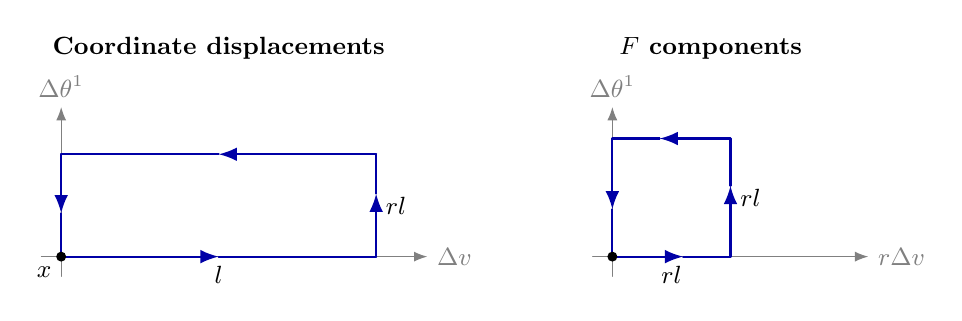
\begin{tikzpicture}[>=Latex,font=\small,line cap=round]
 \begin{scope}[shift={(0,0)}]
  \node[font=\small\bfseries] at (2,2.65) {Coordinate displacements};
  \draw[->,gray] (-.25,0)--(4.65,0) node[right] {$\Delta v$};
  \draw[->,gray] (0,-.25)--(0,1.9) node[above] {$\Delta\theta^1$};
  \draw[blue!65!black,thick,->] (0,0)--(2,0);
  \draw[blue!65!black,thick] (2,0)--(4,0);
  \draw[blue!65!black,thick,->] (4,0)--(4,.8);
  \draw[blue!65!black,thick] (4,.8)--(4,1.3);
  \draw[blue!65!black,thick,->] (4,1.3)--(2,1.3);
  \draw[blue!65!black,thick] (2,1.3)--(0,1.3);
  \draw[blue!65!black,thick,->] (0,1.3)--(0,.55);
  \draw[blue!65!black,thick] (0,.55)--(0,0);
  \fill (0,0) circle (1.8pt) node[below left] {$x$};
  \node[below] at (2,0) {$l$};
  \node[right] at (4,.65) {$rl$};
 \end{scope}
 \begin{scope}[shift={(7,0)}]
  \node[font=\small\bfseries] at (1.25,2.65) {$F$ components};
  \draw[->,gray] (-.25,0)--(3.25,0) node[right] {$r\Delta v$};
  \draw[->,gray] (0,-.25)--(0,1.9) node[above] {$\Delta\theta^1$};
  \draw[blue!65!black,thick,->] (0,0)--(.9,0);
  \draw[blue!65!black,thick] (.9,0)--(1.5,0);
  \draw[blue!65!black,thick,->] (1.5,0)--(1.5,.9);
  \draw[blue!65!black,thick] (1.5,.9)--(1.5,1.5);
  \draw[blue!65!black,thick,->] (1.5,1.5)--(.6,1.5);
  \draw[blue!65!black,thick] (.6,1.5)--(0,1.5);
  \draw[blue!65!black,thick,->] (0,1.5)--(0,.6);
  \draw[blue!65!black,thick] (0,.6)--(0,0);
  \fill (0,0) circle (1.8pt);
  \node[below] at (.75,0) {$rl$};
  \node[right] at (1.5,.75) {$rl$};
 \end{scope}
\end{tikzpicture}
\caption{A coordinate rectangle for $X=\partial_{\theta^1}$, with $u$
and $\theta^2$ fixed (schematic).  Its sides have equal component scale
in $F$, even though their coordinate scales differ.  The proof averages
translated rectangles over all four base-position variables and the
three bounded momentum labels.}
\label{ho:fig-loops}
\end{figure}


\begin{lemma}[Loop jets and the quadratic coefficient]\label{ho:loop-jets}
Uniformly in the observation positions and $X\in\mathcal X$,
\begin{equation}\label{ho:jet-bound}
 \sup_{0\le l\le17l_T}\|\partial_l^{18}H_{x,X}(l)\|\le Q_T.
\end{equation}
The quadratic Taylor coefficient $C_2(x,X)$ of $H_{x,X}(l)-\Id$ is
the matrix, in $F(x)$, of $\pm R(\partial_v,rX)$.  Consequently
\begin{equation}\label{ho:curvature-cancellation}
 g\bigl(C_2(x,X)F_1,X\bigr)
       =\pm R(\partial_v,X,\partial_v,X)=\pm D(X,X).
\end{equation}
The same curvature and loop-orientation convention fixes the signs.
\end{lemma}

\begin{proof}
Since $F$ commutes, its connection coefficients are given by Koszul's
formula
\[
 C^k{}_{ij}=\tfrac12G^{kh}
       (F_iG_{jh}+F_jG_{ih}-F_hG_{ij}).
\]
For a constant column $V$ and $W=rV^iF_i$, the connection matrix on
$W$ is therefore
\begin{equation}\label{ho:koszul-scaled}
 \mathsf A(W)^k{}_j
 =\tfrac12G^{kh}V^i
       \bigl((rF_i)G_{jh}+(rF_j)G_{ih}-(rF_h)G_{ij}\bigr).
\end{equation}
Each $rF_i$ is one of $r\partial_u,\partial_v,r\partial_{\theta^A}$.
Their coefficients are constant and bounded.  Thus the connection
contracted with each of $\partial_v$ and $rX$, and its ordinary
derivatives through order eighteen, are bounded by $Q_T$.
This proves the required cancellation directly, including all shift
and lapse terms; uncontracted $F$ connection coefficients need not
have such a bound.

For an edge parametrized by $s\in[0,1]$, its position has the form
$x+c_e(s,l)$, where $c_e$ is linear in $l$ and independent of momentum.
Its transport equation in $F$ has coefficient
$l\mathsf A(\pm W)(x+c_e(s,l))$ for $W=\partial_v$ or $rX$.
Its integral norm is at most $lQ_T=o(1)$, uniformly in the indicated
range.  Differentiating this coefficient at most eighteen times in
$l$ uses only ordinary derivatives in bounded coordinate directions,
so each derivative is bounded by $Q_T$.
To see the corresponding assertion for transport, differentiate
$P'=-A_eP$, $P(0)=\Id$, $k$ times in $l$:
\[
 (\partial_l^kP)'=-A_e\partial_l^kP
       -\sum_{j=1}^k\binom{k}{j}
            (\partial_l^jA_e)(\partial_l^{k-j}P).
\]
Gronwall uses only the small integral of the undifferentiated $A_e$.
Induction in $k\le18$ bounds every differentiated solution by finite
products of $Q_T$, hence by another subexponential bound.  Multiplying
the four edge transports proves \eqref{ho:jet-bound}.

For completeness, pull the smooth connection back by
$(s,t)\mapsto x+s\partial_v+trX$.  Choose a smooth frame agreeing
with $F$ at $(0,0)$ whose connection one-form vanishes there.
This is possible by prescribing the first derivatives of a frame
change at that point.  On the boundary of $[0,l]^2$ its connection
one-form has integral norm $O(l^2)$.  The ordered transport equals
$\Id$ minus its boundary integral up to $O(l^4)$.  Stokes' theorem
identifies the quadratic coefficient with minus its exterior
derivative at the origin; since the connection form vanishes there,
this is the curvature on $(\partial_v,rX)$, with the orientation sign.
This auxiliary frame is used only to identify a Taylor coefficient,
not to obtain a uniform estimate.
Finally, multilinearity gives
\[
 g\bigl(R(\partial_v,rX)(r^{-1}\partial_v),X\bigr)
       =r r^{-1}R(\partial_v,X,\partial_v,X).
\]
This proves \eqref{ho:curvature-cancellation} with no remaining
factor of $r$.
\end{proof}

\subsection{Averaging before closing the chart estimates}

\begin{proposition}[Averaged holonomy obstruction]
\label{prop:averaged-holonomy}
Assume \eqref{ho:gram-assumptions} on the observation box, bounded
$F$ components of the selected unit tangents, and a fixed bounded
momentum box in \eqref{ho:parameter-measure}. Fix one extension and
one collection of at most $B$ charts with the metric, inverse-metric,
and connection bounds in \Cref{def:exit-test}.
Let $\mathcal G_T\subset\mathcal P_T$ be the measurable parameters
whose base point and unit tangent satisfy the margin and velocity
conditions in at least one chart of this same collection.
There is a measurable exceptional set $\mathcal N_T\subset\mathcal G_T$
such that
\begin{equation}\label{ho:exception-bound}
 \nu_T(\mathcal N_T)\le C e^{-\kappa T/16},
\end{equation}
and, for all parameters in $\mathcal G_T\setminus\mathcal N_T$,
\begin{equation}\label{ho:D-small}
 |D|\le C e^{-13\kappa T/32}+Q_Te^{-\kappa T}
                 =o(\amp).
\end{equation}
The constants use only $B$ and the uniform observation bounds.
\end{proposition}

\begin{proof}
At each good parameter select the least chart index for which the
coordinate margin is at least $1/B$ and $|U_c|\le B$.
The finite selector is measurable and may depend on all three momentum
labels. Fix Borel representatives of the finitely many weak Christoffel
arrays. By \Cref{ho:base-comparison}, the base frame matrices obey
$\|M(0)\|+\|M(0)^{-1}\|\le C_0$.
Choose a fixed $K>2C_0+1$.

Fix $X\in\mathcal X$ and a sampled positive size
$l=j l_T$, $1\le j\le17$.  Use the selected base chart throughout the
four concatenated edges.  Define one first stop on this concatenation:
stop when either $\|M\|=K$ or the chart position has moved Euclidean
distance $1/(2B)$ from its base position.  The latter displacement
keeps the path in the chart because the base margin is $1/B$.
An edge after an earlier stop contributes nothing to any integral
below. Before this global stop the smooth interior path, frame matrix,
and chart coordinates are all defined. More precisely, a parameter is
before the stop at a given time when both strict thresholds hold at
every earlier time in the concatenation. In a fixed chart, continuity
expresses this condition using suprema over rational earlier times, so
it is Borel on the smooth state domain. Intersecting with the measurable
selected parameter set gives the stopped subsets used below.

Write $x=(v,u,\theta)$ and $m=(\pi_u,P)$.  At a fixed edge parameter
$s$ the position is the translation $x\mapsto x+c_e(s,l)$, independent
of $m$.  For the four edges the translations are, successively,
\[
 sl\partial_v,\quad l\partial_v+slrX,\quad
 (1-s)l\partial_v+lrX,\quad (1-s)lrX.
\]
For a selected chart $c$, restrict first to good parameters before
the global stop.  Enlarge this nonnegative integral to all $m\in Q$
and all translated observation positions lying in that chart.  On
positions the translation, the smooth open isometric embedding, and
the chart map compose to an injective smooth coordinate map.  Its
volume change is controlled without estimating its derivative matrix:
isometry and \eqref{ho:volume-density} give
\begin{equation}\label{ho:density-only}
 \dd x\le C r^{-1}\dd\operatorname{vol}_g
       =C r^{-1}\sqrt{|\det\widetilde g_c|}\,\dd y_c
       \le C_B r^{-1}\dd y_c.
\end{equation}
Consequently, for each fixed $s$,
\begin{equation}\label{ho:fixed-edge-average}
 \int_{\substack{\mathcal G_T:\text{chart }c\text{ selected}\\
                         \text{before global stop}}}
 |\widetilde\Gamma_c(y_c(x+c_e(s,l)))|^2\,\dd\nu_T
 \le \frac{C_B|Q|}{r}
                  \int_{c}|\widetilde\Gamma_c(y)|^2\,\dd y.
\end{equation}
Here $\dd\nu_T=\dd x\,\dd m$; no seed Jacobian remains.
The bounded momentum fiber contributes only $|Q|$.
Momentum-dependent chart selection and stop conditions have only
restricted the integral before it was enlarged.  In particular,
\eqref{ho:density-only} has not used the unproved along-edge bound for
$M$.

The weak chart Christoffel array agrees almost everywhere on the open
image with its smooth interior array.  For each $s$, the inverse image
of the exceptional position null set under the preceding smooth
coordinate map is null.  Fubini in $s,x,m$ shows that, outside a null
set of parameters, the stopped trajectory integrals are unchanged by
this choice of representative.  We discard that null set for each of
the finitely many sampled loops.  This justifies the use of the
smooth connection equation below, without asserting a Sobolev trace
on an individually prescribed loop.

Integrate \eqref{ho:fixed-edge-average} in $s\in[0,1]$ and sum the
at most $B$ charts.  If
\[
 I_e(x,m)=\int_0^1\boldsymbol 1_{\{\text{before global stop}\}}
                 |\widetilde\Gamma_c(y_e(s))|\,\dd s,
\]
Cauchy--Schwarz and the chart $L^2$ bounds imply
\begin{equation}\label{ho:L2-average}
             \int_{\mathcal G_T} I_e^2\,\dd\nu_T\le C/r.
\end{equation}
Set $R_T=r^{-1/2}e^{\kappa T/32}$.
Markov's inequality applied to $I_e^2$ gives
\begin{equation}\label{ho:markov}
 \nu_T\{I_e>R_T\}
       \le (C/r)R_T^{-2}=C e^{-\kappa T/16}.
\end{equation}
There are four edges, seventeen positive sizes, and three choices of
$X$.  The union of their exceptional sets, together with the null
sets already removed, satisfies \eqref{ho:exception-bound}.
Only this finite collection is used: no common exceptional set for a
continuum of positive loop sizes is asserted.

We now prove that no stop occurs for a remaining parameter.
On one edge write its $F$-velocity as $f=lrV$, with $V$ a fixed bounded
column, and let $\mathsf A$ be its internal connection matrix.
By \eqref{ho:koszul-scaled}, $|\mathsf A|\le lQ_T$.
The connection transformation law along the smooth interior curve is
the exact matrix equation
\begin{equation}\label{ho:frame-ode}
            M'=M\mathsf A-\widetilde\Gamma_c(Mf)M.
\end{equation}
Here $\widetilde\Gamma_c(Mf)$ means the chart connection matrix
contracted with the chart velocity $Mf$.
Before the stop,
\[
 |M'|\le K lQ_T+C K^2lr|\widetilde\Gamma_c|,
                  \qquad |y'|\le C K lr.
\]
Summing over all four stopped edges and using $I_e\le R_T$ yields
\begin{align}\label{ho:stop-improvement}
 \sup\|M-M(0)\|&\le 4K lQ_T+C K^2lrR_T=o(1),\notag\\
 \sup|y-y(0)|&\le C K lr=o(1).
\end{align}
Indeed $l\le17e^{-\kappa T/16}$ and
$lrR_T\le17e^{-17\kappa T/32}$.
For large $T$ these inequalities are strict improvements of both stop
thresholds.  Continuity rules out a first stop, including on any of
the later three edges.  Thus the entire loop stays in its selected
base chart, with $\|M\|<K$.  Only an upper matrix threshold was needed;
the inverse at the base is already bounded.  If desired, inverse
bounds along the loop also follow from
$\det(M)^2=\det G/\det\widetilde g_c$ and the cofactor formula.

Ordinary chart parallel transport now has total integrated coefficient
at most $C lr\sum_e I_e\le C lr^{1/2}e^{\kappa T/32}$.
Its matrix differs from $\Id$ by at most the exponential of this
quantity minus one.  Since the rectangle closes exactly, its final
frame matrix equals its base matrix.  Thus if $P_c$ is the full chart
transport, $H=M(0)^{-1}P_cM(0)$.  Conjugating by the bounded base matrix
and its inverse gives
\begin{equation}\label{ho:sampled-holonomy}
 \|H_{x,X}(j l_T)-\Id\|
       \le C r^{1/2}l_T e^{\kappa T/32},
                     \qquad 1\le j\le17.
\end{equation}
At $j=0$ the left side is zero.  All transports in this argument have
taken place in the smooth original spacetime.

It remains to extract the quadratic coefficient from these eighteen
values.  We include the elementary interpolation argument, as in
\cite[\CompanionRef{signed}{holo:interpolation}]{KerrCOne}.  Write
\[
 H_{x,X}(l)-\Id=\sum_{k=0}^{17}C_k l^k+\mathcal R_{18}(l).
\]
By \Cref{ho:loop-jets}, the Taylor integral remainder at $l=j l_T$
is bounded by $C Q_Tl_T^{18}$.  The Vandermonde matrix
$(j^k)_{0\le j,k\le17}$ is invertible and independent of $T$.
Therefore its inverse expresses $l_T^2 C_2$ as a fixed linear
combination of the values of the polynomial at these nodes, giving
\begin{align}\label{ho:coefficient-estimate}
 \|C_2\|
 &\le C l_T^{-2}\max_{0\le j\le17}
                       \|H_{x,X}(j l_T)-\Id\|+Q_Tl_T^{16}\notag\\
 &\le C r^{1/2}l_T^{-1}e^{\kappa T/32}+Q_Tl_T^{16}\notag\\
 &=C e^{-13\kappa T/32}+Q_Te^{-\kappa T}.
\end{align}
Both exponents have a strict gain over $-\kappa/4$.
By \eqref{ho:curvature-cancellation} and boundedness of $G$, this
controls $D(X,X)$ for each $X\in\mathcal X$.
Curvature pair symmetry gives $D_{12}=D_{21}$, and
\[
 2D_{12}=D(\partial_{\theta^1}+\partial_{\theta^2},
                \partial_{\theta^1}+\partial_{\theta^2})
             -D_{11}-D_{22}.
\]
These three estimates prove \eqref{ho:D-small} for the entire
symmetric $2\times2$ block.
\end{proof}

\subsection{Finite persistence and nowhere denseness}

The preceding estimate makes the observed curvature block small on
almost every parameter with an extension-chart witness. To contradict
the packet signal, we will apply it to the original datum and a nearby
datum at identical numerical terminal states. Canonical section volume
ensures that their two good families still overlap.

\Cref{prop:matched-seeds} supplies the needed persistence for each
fixed finite experiment: a relative open neighborhood preserves the
signal with lower bound $\amp$, the frame and finite-jet bounds, and
the injective measure-preserving backward maps into $O$. Its map
tolerance can be chosen after $T$, and its data-neighborhood radius
may depend on that experiment. The next argument uses precisely this
finite persistence.

\begin{theorem}[Nowhere denseness of the extension tests]
\label{thm:nowhere-dense}
For the single neighborhood $\Ueps$ fixed in
\Cref{prop:bg-package}, every set $E(O,B)$ of \Cref{def:exit-test} is
relatively nowhere dense in $\Ueps$.
\end{theorem}

\begin{proof}
Suppose instead that a nonempty relative open set $V\subset\Ueps$
is contained in $\overline{E(O,B)}$.  Since $E(O,B)$ is dense in $V$,
choose $d\in E(O,B)\cap V$.
The weighted seminorms are increasing, so there are a finite $m\ge10$
and $\eta>0$ such that
\begin{equation}\label{ho:finite-neighborhood}
        \{d'\in\Ueps:p_m(d'-d)<\eta\}\subset V.
\end{equation}
Fix the branch tube and the extension witness belonging to this datum.
Apply the finite packet construction at order $m$, along its unbounded
sequence of admissible observation times.  By
\Cref{prop:packet-preparation,thm:dn-comparison,prop:experiment-attachment},
the exact full-bridge data $d_T$ satisfy $p_m(d_T-d)\to0$; hence they
lie in $V$ for all sufficiently large $T$.

The set $E(O,B)$ is dense in $V$, so \Cref{prop:matched-seeds}
allows us, for every such fixed $T$, to choose
$\widehat d_T\in E(O,B)\cap V$ as close to $d_T$ as required by all the
finite observation conditions.  We also require
$p_0(\widehat d_T-d_T)\to0$.  Write $\widehat g_T$ for its observed
metric.  We then have, on the common position tube,
\begin{equation}\label{ho:persisted-signal}
 |D(\widehat g_T)-D(g_d)|>\amp
                 \quad\text{if }|\cos(\lambda v)|\ge1/2,
\end{equation}
and both metrics have the uniform hypotheses of
\Cref{prop:averaged-holonomy}.  In particular the constants there are
independent of $T$; the required finite closeness was chosen to retain
them.  Smooth dependence of the initial section density on $h$ gives
\begin{equation}\label{ho:initial-measure-ratio}
                  \frac{\mu_{\widehat d_T}(O)}{\mu_d(O)}\longrightarrow1.
\end{equation}

Let $S\subset O$ and $\widehat S_T\subset O$ be the good seed families
in the two existential extension witnesses.  Each has more than
$99$ percent of its respective measure of $O$.
Use \eqref{ho:parameter-measure} for the background hits of $O_0$.
At a fixed $v$, the loss from parameters whose background seed is
outside $S$ is at most $.01\mu_d(O)$.
The matched backward map for $\widehat g_T$ is injective into $O$ and
preserves its canonical section measure.  Its loss from
$O\setminus\widehat S_T$ is therefore at most
$.01\mu_{\widehat d_T}(O)$.
By \eqref{ho:initial-measure-ratio}, their combined loss is less than
$.04\mu_d(O)$ for large $T$, uniformly on every $v$ slice.  Thus, if
$\mathcal G_T^{\cap}$ denotes parameters good for both metrics,
\begin{equation}\label{ho:joint-good-slice}
 \operatorname{vol}_6(\mathcal G_T^{\cap}\cap\{v=\text{constant}\})
       >(.95-.04)\mu_d(O)=.91\mu_d(O).
\end{equation}
The dependence on $v$ is measurable by the smooth finite flow maps.
The chart bounds from either witness apply at these observations
because \Cref{def:exit-test} imposes them throughout the full future
geodesic lifetime, and the matched observations are interior points
of that geodesic.

Let
\[
 I_T=\{v\in T+J_0:|\cos(\lambda v)|\ge1/2\}.
\]
The condition occupies $2/3$ of each full period.  Only the two end
periods of an interval can be incomplete, so
$|I_T|=\frac23|J_0|+O(\lambda^{-1})>\frac12|J_0|$ for large $T$.
Integration of \eqref{ho:joint-good-slice} over $I_T$ gives
\begin{equation}\label{ho:positive-intersection}
 \nu_T(\mathcal G_T^{\cap}\cap\{v\in I_T\})
                    >.455\mu_d(O)|J_0|.
\end{equation}
Apply \Cref{prop:averaged-holonomy} separately to $g_d$ and
$\widehat g_T$.  The union of the two additional exceptional sets has
measure tending to zero.  It cannot cover
\eqref{ho:positive-intersection}.  At a remaining parameter both
$|D(g_d)|$ and $|D(\widehat g_T)|$ are $o(\amp)$, uniformly, whereas
\eqref{ho:persisted-signal} says their difference exceeds $\amp$.
This is a contradiction.

We have excluded nonempty interior of $\overline{E(O,B)}$.
No closedness of $E(O,B)$ was assumed.
\end{proof}

\begin{proof}[Proof of \Cref{thm:main}]
By \Cref{prop:exit-cover}, every datum in $\Ueps$ admitting the future
extension in the statement belongs to some $E(O,B)$.
The seed basis and the positive integers $B$ are countable.
By \Cref{thm:nowhere-dense}, their union is meagre in the full relative
weighted smooth topology on $\Ueps$.  Explicitly,
\[
 \mathcal R=\bigcap_{O,B}\bigl(\Ueps\setminus\overline{E(O,B)}\bigr)
\]
is a countable intersection of relatively open dense sets and consists
of future-inextendible data.
The exit cover concerns all future exits of the full developments.
Every background observation precedes the corresponding geodesic's
first comparison runout. The exact and persisted observations lie in finite interior
regions of their full developments, where the full-lifetime chart
witnesses apply. Thus the conclusion excludes every extension specified
in \Cref{thm:main}, for this single $p_{10}$ neighborhood.
\end{proof}

\bibliographystyle{plain}
\bibliography{refs/sources}
\end{document}
